\documentclass[a4paper,10pt]{report}
\usepackage{geometry}\geometry{a4paper,top=3.5cm,bottom=3.5cm,%
left=2.5cm,right=2.5cm,heightrounded,bindingoffset=0mm}
\usepackage[T1]{fontenc}
\usepackage[utf8]{inputenc}
\usepackage[italian]{babel}
\usepackage{graphicx}
\usepackage{subfig}
\usepackage{amsmath,amsfonts,amssymb,braket,mathrsfs}
\usepackage{float}
\usepackage{tabularx,booktabs}
\usepackage{hyperref}
\usepackage{epsfig}
%\usepackage{minipage}
\usepackage[output-decimal-marker={,}]{siunitx}
\usepackage{tikz}
\usepackage{pgfplots,pgfplotstable}
\pgfplotsset{compat=1.15} %indica la versione da utilizzare per pgfplot
\usetikzlibrary{patterns} % per il tratteggio
\usepackage{stanli}
\usepackage{xspace}% per lo spazio intelligente
\newcommand{\e}{\`E\xspace}  %E'
\usepackage{titlesec} % per formato custom dei titoli dei capitoli
%\usepackage{sideways}%%%
% redefinizione del formato del titolo del capitolo
      % da formato
      %   Capitolo X
      %   Titolo capitolo
      %   a formato
      %      Titolo capitolo 
	\titleformat{\chapter}
        {\normalfont\Huge\bfseries}{}{0em}{}
	\titlespacing*{\chapter}{0pt}{0in}{0.02in}
	\titlespacing*{\section}{0pt}{0.2in}{0.02in}
	\titlespacing*{\subsection}{0pt}{0.10in}{0.02in}
%serve per la didascalia di tabelle e figure:
\usepackage{caption}
\captionsetup{tableposition=top,figureposition=bottom,font=small}\captionsetup{format=hang,labelfont={bf,color=pantone186}} %didascalie a più righe allineate e il nome in grassetto
%non viene allineato a sinistra se la didascalia è corta una sola riga. PERCHé??
\usepackage{xcolor}
%serve per mettere il codice con lo sfondo grigio chiaro
\definecolor{pantone186}{RGB}{206, 17, 38} %il colore del logo UNITN
\usepackage{listings} 
\lstset{basicstyle=\scriptsize\ttfamily,
backgroundcolor=\color{lightgray},%
boxpos=c,%
stringstyle=\itshape,		
lineskip=3pt,%
numbers=left,
numberstyle=\tiny,}
\usepackage{lscape}
\usepackage{multirow}
\usepackage{import}
\begin{document}
%!TEX root = ../RelazioneStrutturaleMeoliNicola.tex
\pagestyle{plain}
\thispagestyle{empty}
\begin{center}
  \begin{figure}[H]
    \centerline{
\psfig{file=IMG/logo_unitn_black_center.eps,
                        width=0.8\textwidth,trim = 0 0.9cm 0 0.5cm}}
  \end{figure}
\line(1,0){450}

  \Large\textsc{Dipartimento di Ingegneria Civile, Ambientale e Meccanica\\}
  \Large{Corso di Laurea in Ingegneria Civile
  }

  \vspace{2.7 cm} 
  %\Large\textsc{Elaborato finale\\} 
  %\vspace{1 cm} 
  \Huge\textsc{relazione di meccanica computazionale delle strutture 1\\}
  
  \vspace{0.5 cm}
  \Large{\it{Risoluzione di una struttura iperstatica tramite diversi metodi di calcolo \\ Risoluzione di una lastra soggetta ad una tensione assiale}}


  \vspace{3 cm} 
  \begin{tabular*}{\textwidth}{ l @{\extracolsep{\fill}} r }
  \Large\textsc{Docenti} & \Large\textsc{Studenti}\\
  \Large{Massimo Penasa}& \Large{Angelica Lenzi 173852}\\
  \Large{Andrea Piccolroaz} & \Large{Nicola Meoli 186100}\\
  \Large{Matteo Tommaselli}	 & \\
  	
  	
  \end{tabular*}

  \vspace{3.5cm} 
    \line(1,0){450}
    
  \Large{Anno accademico 2018/19}
  
\end{center}


\tableofcontents
%\setcounter{page}{1}
%Tabelle e figure sulla stessa pagina:
%Le aggiunge all'indice. phantomsection serve per non far casini con hyperref
\clearpage
\begingroup
   %\let\cleardoublepage\relax  % book
    \let\clearpage\relax        % report
        \listoftables
        \phantomsection
        \addcontentsline{toc}{chapter}{Elenco delle tabelle}
        %
        \listoffigures
        \phantomsection
        \addcontentsline{toc}{chapter}{Elenco delle figure}
\endgroup
%
%
\newcommand{\norma}[1]{\textsc{#1}}
\newcommand{\normaref}[1]{\texttt{#1}}
%!TEX root = ../RelazioneStrutturaleMeoliNicola.tex
\chapter{Relazione strutturale}
%!TEX root = ../RelazioneStrutturaleMeoliNicola.tex
\chapter{Trave P13-P18-Ascensore -- Piano primo}
%!TEX root = ../RelazioneStrutturaleMeoliNicola.tex
\begin{figure}[htb]
\centering
\begin{tikzpicture}
\scaling{0.55};
	\point{n1}{00.00}{0};
	\point{n2}{03.00}{0};
	\point{n3}{07.50}{0};
	\point{n4}{11.50}{0};
	\point{n5}{16.50}{0};
	\point{n6}{22.65}{0};
	\point{n7}{26.65}{0};
	\beam{2}{n1}{n2}[0][1];
	\beam{2}{n2}{n3}[1][1];
	\beam{2}{n3}{n4}[1][1];
	\beam{2}{n4}{n5}[1][1];
	\beam{2}{n5}{n6}[1][1];
	\beam{2}{n6}{n7}[1][1];
	\begin{scope}[scale=0.6]
		\support{1}{n1};
		\support{1}{n2};
		\support{1}{n3};
		\support{1}{n4};
		\support{1}{n5};
		\support{1}{n6};
		\support{3}{n7}[90];
	\end{scope};	
	\dimensioning{1}{n1}{n2}{-1.5}[$\SI{3.00}{\meter}$];
	\dimensioning{1}{n2}{n3}{-1.5}[$\SI{4.50}{\meter}$];
	\dimensioning{1}{n3}{n4}{-1.5}[$\SI{4.00}{\meter}$];
	\dimensioning{1}{n4}{n5}{-1.5}[$\SI{5.00}{\meter}$];
	\dimensioning{1}{n5}{n6}{-1.5}[$\SI{6.15}{\meter}$];
	\dimensioning{1}{n6}{n7}{-1.5}[$\SI{4.00}{\meter}$];
	%Nomi dei punti
	\notation{4}{n1}{n2}[$1$];
	\notation{4}{n2}{n3}[$2$];
	\notation{4}{n3}{n4}[$3$];
	\notation{4}{n4}{n5}[$4$];
	\notation{4}{n5}{n6}[$5$];
	\notation{4}{n6}{n7}[$6$];
	%
	\point{m1}{00.00}{-1.5};
	\point{m2}{03.00}{-1.5};
	\point{m3}{07.50}{-1.5};
	\point{m4}{11.50}{-1.5};
	\point{m5}{16.50}{-1.5};
	\point{m6}{22.65}{-1.5};
	\point{m7}{26.65}{-1.5};
	\notation{6}{m1}{$1$};
	\notation{6}{m2}{$2$};
	\notation{6}{m3}{$3$};
	\notation{6}{m4}{$4$};
	\notation{6}{m5}{$5$};
	\notation{6}{m6}{$6$};
	\notation{6}{m7}{$7$};
\end{tikzpicture}
\caption{Schema strutturale adottato e relativa nomenclatura utilizzata}
\label{fig:Struttura0}
\end{figure}
\section{Analisi dei carichi trave}
\subsection{Peso proprio trave}
La trave è di sezione rettangolare $30 \times \SI{50}{\centi\metre}$ in calcestruzzo armato. 
La normativa in \normaref{Tab. 3.1.II} suggerisce di utilizzare un peso specifico $\gamma_{CLS}$ pari a \SI{25.0}{\kilo\newton\per\meter\cubed} per il calcestruzzo armato. 
Pertanto il carico lineare risulta 
\[
	G_1^{trave} = 0.3 \cdot 0.5 \cdot 25 = \SI{3.75}{\kilo\newton\per\meter}
\]

\subsection{Terrazzo}
\paragraph*{Carichi permanenti G1}
Come da progetto il peso del solaio ultimato in travetti tralicciati in latero cemento è pari a $g_1^{ter.}=\SI{3.20}{\kilo\newton\per\square\meter}$.
\paragraph*{Carichi permanenti non strutturali G2}
Il carico distribuito su superficie permanente non strutturale agente sul terrazzo è la somma dei singoli carichi degli strati che compongono la stratigrafia presente.
\begin{center}
\begin{tabular}{lS[table-format=2.1]S[table-format=1.2]S[table-format=1.3]}
	\toprule
	\multirow{2}{*}{Strato} & \multicolumn{1}{c}{Peso specifico} & \multicolumn{1}{c}{Spessore}& \multicolumn{1}{c}{$g_{2,k}$}\\
    	   & \multicolumn{1}{c}{$\left[\SI{}{\kilo\newton\per\meter\cubed}\right]$} & \multicolumn{1}{c}{$\left[\SI{}{\meter}\right]$}& \multicolumn{1}{c}{$\left[\SI{}{\kilo\newton\per\square\meter}\right]$}\\
	\midrule
	Isolante 	             & 0.5  & 0.15 & 0.075 \\
	Massetto calcestruzzo 	 & 24.0 & 0.06 & 1.44  \\
	Pavimento 	             &      &      & 0.50  \\
	Intonaco intradosso 	 & 20.0 & 0.01 & 0.20 \\
	\midrule
	Totale $g_2^{ter.} =$ &&&2.215\\
	\bottomrule
\end{tabular}
\end{center}
\paragraph*{Categoria B - balconi} Si è supposto che la funzione del terrazzo sia equiparabile strutturalmente a quella di un balcone. 
La \normaref{Tab. 3.1.II} delle \norma{NTC2018} prevede per i balconi un carico distribuito pari a \SI{4.00}{\kilo\newton\per\square\meter}
\paragraph*{Neve}
L'edificio è ubicato in zona 1 ad una quota superiore a \SI{200}{\meter} pertanto il valore di riferimento del carico della neve al suolo risulta pari a
\[
	q_{sk}=1.39 \, [1+(a_s/728)^2] = \SI{1.626}{\kilo\newton\per\square\meter}
\]

Si assume che l'edificio sia in zona normale di vento. Pertanto $C_E$ risulta pari a $1$.
Si assume un coefficiente termico $C_t = 1$ in quanto è assente uno specifico studio riguardo la perdita di calore della costruzione. 

\begin{figure*}[htb]
\centering
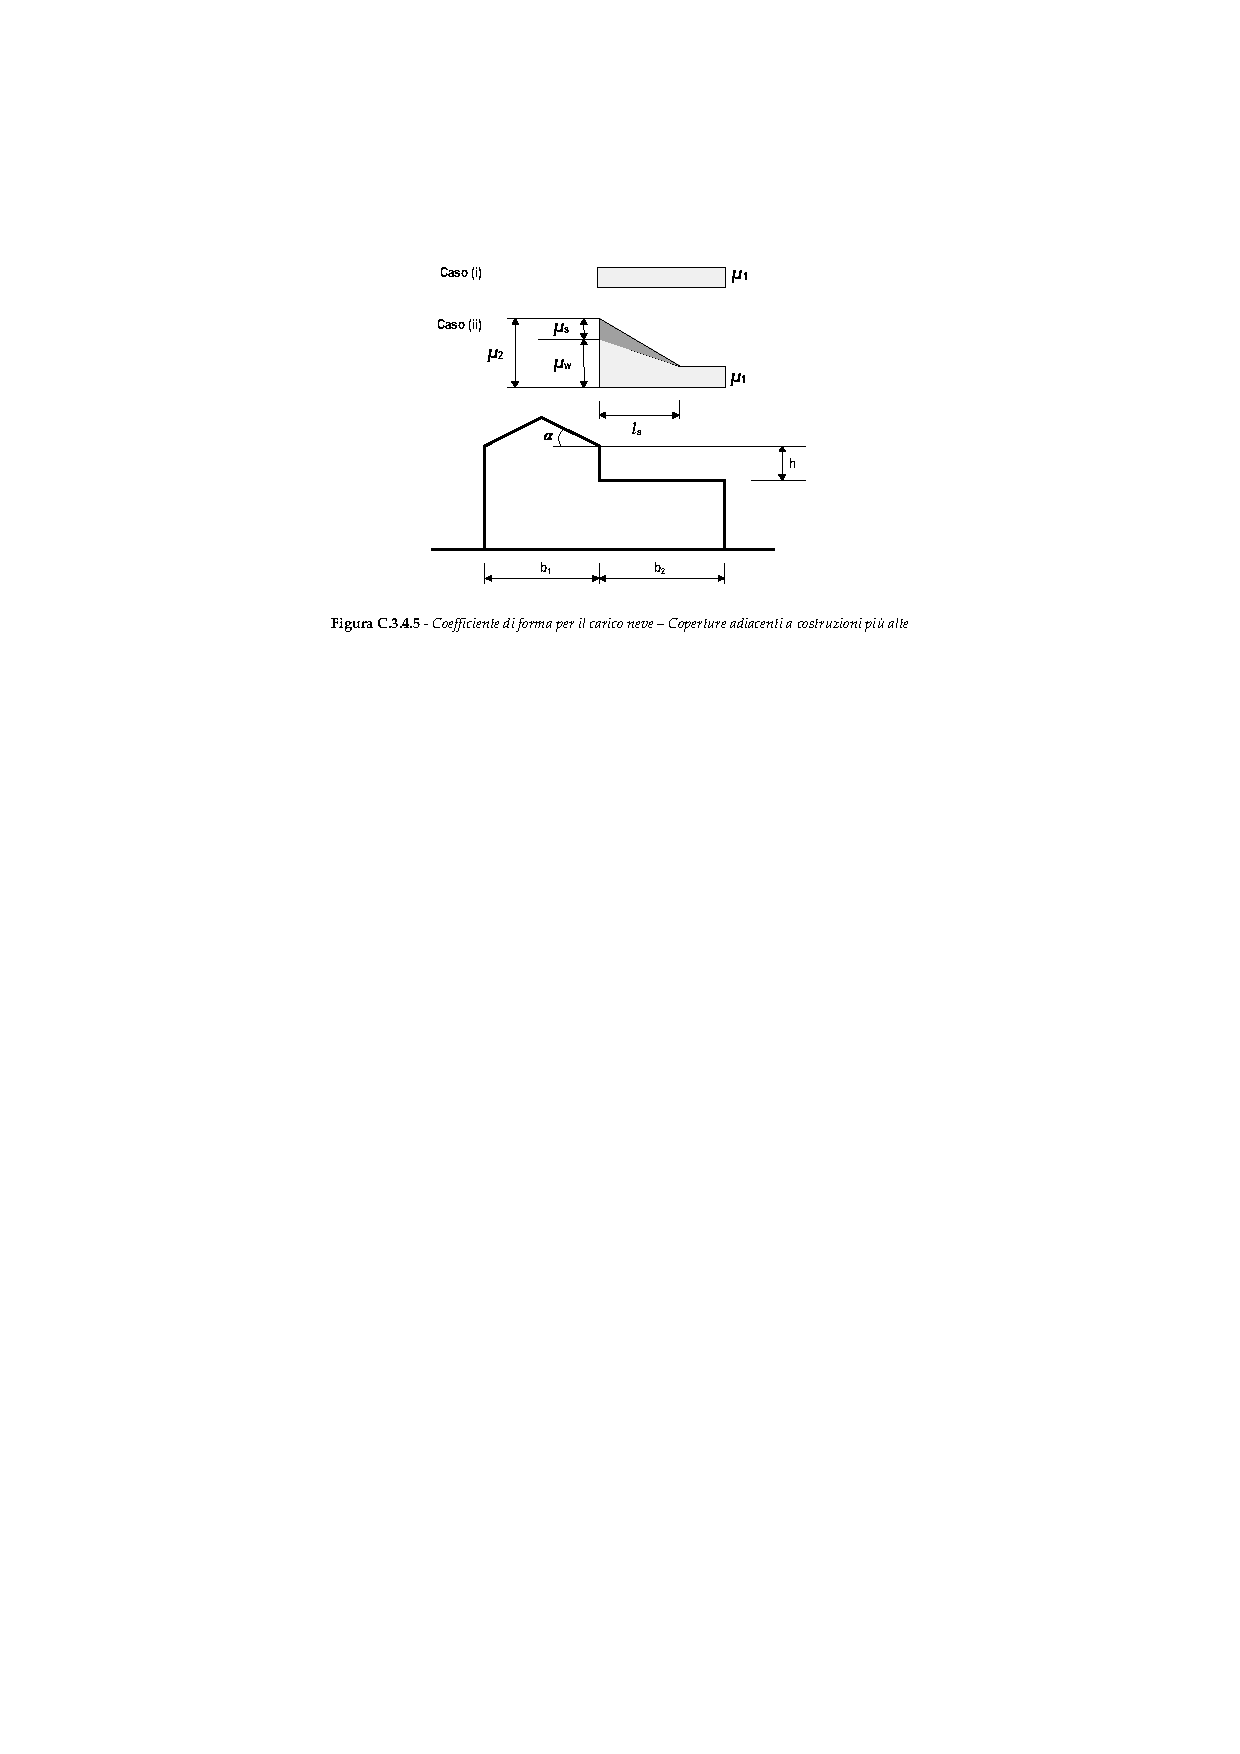
\includegraphics{IMG/figC3-4-5.pdf}
\label{fig:C345}
\end{figure*}
Per il calcolo del coefficiente di forma $\mu_i$ la \norma{circolare} in \normaref{Fig. C.3.4.5} (riportata a pagina \pageref{fig:C345}) prevede due possibili casi dovuti alla vicinanza della copertura a costruzioni più alte in quanto si genera un accumolo di neve.
Il primo caso prevede $\mu_1=0.8$ ed è costante data la copertura piana. Nel secondo caso $\mu_2$ è la somma tra il contributo $\mu_s$ dello scivolamento della neve dalla copertura al piano superiore e pertanto è nullo essendo piana anch'essa. 
E il contributo $\mu_w$ dovuto al vento che redistribuisce la neve. 
Questo vale $\mu_w=\frac{b_1 + b_2}{2\,h}$: si hanno quindi due casi dovuti alla diversa dimensione di $b_2$ che vale \SI{6.00}{} e \SI{3.50}{\meter} rispettivamente tra le zone indicate in FIGURA DA METTERE.
Gli altri termini invece valgono $b_1=\SI{18.00}{\meter}$ e $h=\SI{6.20}{\meter}$. 
Si ottiene $\mu_w^1=1.935$ e $\mu_w^2=1.734$.

Essendo $l_s=2\,h>b_2$ in entrambi i casi, il coefficiente $\mu$ deve essere interpolato in base alla lunghezza $b_2$. 
Usando la similitudine dei triangoli come mostrato in FIGURA DA METTERE si ottiene l'altezza del triangolo a distanza $b_2$ dall'edificio e che sommato al valore dell'altezza $\mu_1$ del rettangolo porta al valore del \normaref{caso 2} cercato 
\begin{align*}
	\mu_2^{1}=&\mu_1 + \frac{(l_s - b_2^1)\cdot (\mu_w^1-\mu_1)}{l_s} = 1.386\\
	\mu_2^{2}=&\mu_1 + \frac{(l_s - b_2^2)\cdot (\mu_w^2-\mu_1)}{l_s} =	1.470
\end{align*}
Per semplicità si assume ora un valore unico del coefficiente tra i valori delle altezze del trapezio del caso 2 e pari alla media tra $\mu_2$ e $\mu_w$ ottenendo $\mu^1= 1.661$ e $\mu^2=1.602$ e costante.

Il carico dovuto alla neve sul terrazzo risulta infine pari a 
\begin{align}
q_s^1 &= q_{sk} \cdot C_E \cdot C_t \cdot \mu^1 = \SI{1.626}{} \cdot 1 \cdot 1 \cdot 1.661 = \SI{2.700}{\kilo\newton\per\square\meter}\\
q_s^2 &= q_{sk} \cdot C_E \cdot C_t \cdot \mu^2 = \SI{1.626}{} \cdot 1 \cdot 1 \cdot 1.602 = \SI{2.605}{\kilo\newton\per\square\meter}\label{eq:qneve}
\end{align}
\paragraph*{Vento} \label{cap:ventoTerrazzo} 
La velocità base di riferimento $V_b$ è data dalla \normaref{3.3.1} delle \norma{NTC2018} e dalla relativa \normaref{Tab. 3.3.1} nel quale il coefficiente di altitudine $c_a$ vale $1$ perché la quota è inferiorie ad $a_0$ e $V_{b,o}=\SI{25}{\meter\per\second}$. 
Il coefficiente di ritorno $c_r$ della \normaref{formula 3.3.2} è pari a $1$ nel caso di un tempo pari a 50 anni. 
Pertanto la velocità di riferimento $V_r=\SI{25}{\meter\per\second}$.
Assumendo una densità dell'aria $\rho$ come consigliato nel \normaref{\S 3.3.6}, la pressione cinetica di riferimento vale $q_r =1/2\, \rho\, V_r^2 = \SI{0.39}{\kilo\newton\per\square\meter}$. 

L'edificio è ubicato in provincia di Trento pertanto è in zona urbana ad una quota inferiore a \SI{500}{\meter} ed ad una distanza maggiore di \SI{30}{\kilo\meter} dal mare. 
Risulta quindi dalla \normaref{Tab. 3.3.III} una classe di rugosità del terreno A e dalla \normaref{Fig. 3.3.2} una classe di esposizione V del sito.
Pertanto dalla \normaref{Tab. 3.3.II} si ha
\[
	k_r=0.23 \qquad z_0=\SI{0.70}{\meter} \quad z_{min}=\SI{12}{\meter}
\]
Il coefficiente di topografia $c_t$ è assunto pari a $1$.
La quota del terrazzo in cui si sta calcolando l'azione del vento è pari a \SI{3.50}{\meter}.
Il coefficiente di esposizione risulta pari alla \normaref{formula 3.3.7} 
\[
	c_e(z)=c_e(z_{min})=k_t^2\cdot c_t \cdot \ln(z/z_0)\cdot[7+c_t\cdot\ln (z/z_0)] = 1.48
\]

Per il calcolo del coefficiente di pressione $c_p$ si è preso come riferimento il \normaref{\S C3.3.8.1.2} riguardante le coperture piane non essendo elencati nelle normative casi specifici per i terrazzi.

Si sono utilizzati i coefficienti globali in quanto si vuole calcolare la pressione o depressione complessiva esercitata dalla forza del vento. 
Si avranno due valori di pressione positivi e negativi e che verranno usati per ottenere poi (nel paragrafo \ref{cap:combinazioniCarico}) i valori sfavorevoli e favorevoli.

Per il calcolo del coefficiente $C_{pe}$ la \norma{circolare} propone la distinzione di due zone A e B, la prima avente dimensione $\min\{ b/2\,;\,h\}$ che nel caso in esame è pari a $\min\{\frac{\SI{33.65}{\meter}}{2};\SI{3.50}{\meter}\}=\SI{3.50}{\meter}$.
Essendo quindi il terrazzo delimitato da entrambe le zone e non volendo calcolare la forza totale del vento ma il carico su superficie, si è considerato nel caso di pressione il coefficiente positivo $C_{pe,B}=+0.2$ da usare nel caso sfavorevole e il coefficiente negativo $C_{pe,B}=-0.20$ da usare nel caso favorevole di depressione.
Quest'ultimo in realtà a favore di sicurezza in quanto sarebbe da considerare anche il coefficiente $C_{pe,A}=-0.80$.

Il coefficiente dinamico $c_d$ è preso pari ad 1 come suggerito nel capitolo \normaref{\S 3.3.9}

Pertanto il carico dovuto al vento è pari a 
\[
	q_w = q_r \cdot c_e \cdot c_p \cdot c_d = \SI{0.39}{\kilo\newton\per\square\meter}\cdot 1.48 \cdot \pm 0.20 \cdot 1= \pm \SI{0.1154}{\kilo\newton\per\square\meter}
\]
\subsection{Interno}
\paragraph*{Carichi permanenti strutturali G1}
\e presente il medesimo solaio strutturale del terrazzo, pertanto $g_1^{sol.}=\SI{3.20}{\kilo\newton\per\square\meter}$.
\paragraph*{Carichi permanenti non strutturali G2}\label{cap:g2Trave} Sono costituiti dal pacchetto non strutturale della stratigrafia del solaio e dalle pareti divisorie interne. 
Per quanto riguarda le pareti divisorie interne il \normaref{\S 3.1.3} delle \norma{NTC2018} permette di spalmare il peso delle pareti interne in un carico distribuito su tutta la superficie.
\begin{center}
\begin{tabular}{lS[table-format=2.1]S[table-format=1.2]S[table-format=1.3]}
	\toprule
	\multirow{2}{*}{Strato} & \multicolumn{1}{c}{Peso specifico} & \multicolumn{1}{c}{Spessore}& \multicolumn{1}{c}{$g_{2,k}$}\\
    	   & \multicolumn{1}{c}{$\left[\SI{}{\kilo\newton\per\meter\cubed}\right]$} & \multicolumn{1}{c}{$\left[\SI{}{\meter}\right]$}& \multicolumn{1}{c}{$\left[\SI{}{\kilo\newton\per\square\meter}\right]$}\\
	\midrule
	Tramezze in laterizio 	 	 & 8.00 & 0.08 & 0.64 \\
	Intonaco interno 	     	 & 20.0 & 0.01 & 0.2 \\
	Intonaco esterno	         & 20.0 & 0.01 & 0.2 \\
	\midrule
	Totale $=$   				 &      &      & 1.04 \\
	\bottomrule
\end{tabular}
\end{center}
L'altezza delle pareti corrisponde all'altezza di interpiano meno lo spessore del solaio, il che risulta $\SI{3.10}{} - \SI{0.25}{} = \SI{2.85}{\meter}$.
Il carico lineare delle pareti interne diviene quindi \SI{2.964}{\kilo\newton\per\meter}.
Utilizzando la normativa si ottiene così un carico di \SI{1.20}{\kilo\newton\per\square\meter}.

Unendo tutti i contributi si ha 
\begin{center}
\begin{tabular}{lS[table-format=2.1]S[table-format=1.2]S[table-format=1.3]}
	\toprule
	\multirow{2}{*}{Strato} & \multicolumn{1}{c}{Peso specifico} & \multicolumn{1}{c}{Spessore}& \multicolumn{1}{c}{$g_{2,k}$}\\
    	   & \multicolumn{1}{c}{$\left[\SI{}{\kilo\newton\per\meter\cubed}\right]$} & \multicolumn{1}{c}{$\left[\SI{}{\meter}\right]$}& \multicolumn{1}{c}{$\left[\SI{}{\kilo\newton\per\square\meter}\right]$}\\
	\midrule
	Sottofondo CLS alleggerito 	 & 16.0 & 0.08 & 1.28 \\
	Massetto allettamento 	     & 24.0 & 0.06 & 1.44 \\
	Pavimento ceramica 	         &      &      & 0.50 \\
	Intonaco intradosso 	     & 20.0 & 0.01 & 0.20 \\
	Pareti interne distribuite   &      &      & 1.20 \\
	\midrule
	Totale $g_2^{sol.} =$        &      &      & 4.62 \\
	\bottomrule
\end{tabular}
\end{center}
\paragraph*{Categoria B - Uffici} La \normaref{Tab. 3.1.II} prevede un carico variabile di \SI{3.00}{\kilo\newton\per\square\meter} per la categoria uffici.
\subsection{Pareti perimetrali}
Sono agenti direttamente con un carico lineare al di sopra della trave e si estendono per una altezza pari a quella di interpiano meno la trave.
Ovvero $\SI{3.10}{} - \SI{0.5}{} = \SI{2.60}{\meter}$.
\begin{center}
\begin{tabular}{lS[table-format=2.1]S[table-format=1.2]S[table-format=1.3]}
	\toprule
	\multirow{2}{*}{Strato} & \multicolumn{1}{c}{Peso specifico} & \multicolumn{1}{c}{Spessore}& \multicolumn{1}{c}{$g_{2,k}$}\\
    	   & \multicolumn{1}{c}{$\left[\SI{}{\kilo\newton\per\meter\cubed}\right]$} & \multicolumn{1}{c}{$\left[\SI{}{\meter}\right]$}& \multicolumn{1}{c}{$\left[\SI{}{\kilo\newton\per\square\meter}\right]$}\\
	\midrule
	Muratura in laterizio 	 	 & 10   & 0.30 & 3 \\
	Intonaco interno 	     	 & 20.0 & 0.01 & 0.2 \\
	Cappotto esterno	         & 0.20 & 0.12 & 0.024 \\
	\midrule
	Totale $=$   				 &      &      & 3.224 \\
	\bottomrule
\end{tabular}
\end{center}
\[
G_2^{pareti}=\SI{3.224}{\kilo\newton\per\square\meter} \cdot \SI{2.60}{\meter} = \SI{8.382}{\kilo\newton\per\meter}
\]
\section{Totale carichi agenti sulla trave}
Vengono ora moltiplicati i risultati appena trovati per le relative lunghezze di influenza. 
Si è diviso il problema in tre zone: A, B e C come mostrato in FIGURA DA METTERE. 
Nella zona A e B si ha una zona esterna dell'edificio e una zona interna.
Pertanto si considera il carico gravante sulla trave in oggetto di calcolo spalmato sui $5/8$ della luce nella zona verso l'esterno e alla metà della luce nella zona sottostante.  
Diviene rispettivamente pari a 
\begin{align*}
	\text{A :}&\qquad L^{ter.}=\frac{5}{8}\cdot\SI{6.00}{\meter}=\SI{3.75}{\meter} \qquad 
				L^{sol.} \frac{1}{2}\cdot\SI{5.00}{\meter} = \SI{2.50}{\meter}\\
	\text{B :}&\qquad L^{ter.}=\frac{5}{8}\cdot\SI{3.50}{\meter}=\SI{2.19}{\meter} \qquad 
				L^{sol.} \frac{1}{2}\cdot\SI{5.00}{\meter} = \SI{2.50}{\meter}\\
\end{align*}
Nella zona C invece l'orditura del solaio del terrazzo al primo piano è nell'altra direzioni. 
A tal proposito si considera una lunghezza di influenza del terrazzo simbolica di \SI{1.00}{\meter}.
Nella parte sottostante è uguale a quella delle altre zone.
\[
	\text{C :}\qquad L^{ter.}=\SI{1.00}{\meter} \qquad 
				L^{sol.} \frac{1}{2}\cdot\SI{5.00}{\meter} = \SI{2.50}{\meter}
\]

I carichi a metro lineare sotto riportati tenendo conto di tali lunghezze e sono stati combinati con le relativi azioni agenti sulla trave.

Nel caso dei sovraccarichi variabili si è assunta l'ipotesi che essi agiscano sempre insieme. 
Ovvero quando è possibile che avvenga il valore caratteristico nel terrazzo, questo avverrà anche nel solaio interno.
\paragraph*{Zona A} 
\[
\begin{split}
G_1^A &=  g_1^{ter.}\cdot L^{ter.} + g_1^{sol.}\cdot L^{sol.} + G_1^{trave} \\
&= \SI{3.20}{\kilo\newton\per\square\meter}\cdot\SI{3.75}{\meter} + \SI{3.20}{\kilo\newton\per\square\meter}\cdot\SI{2.50}{\meter} + \SI{3.75}{\kilo\newton\per\meter} \\
&= \SI{23.75}{\kilo\newton\per\meter} \\
G_2^A &= g_2^{ter.}\cdot L^{ter.} + g_2^{sol.}\cdot L^{sol.} + G_2^{pareti} \\
&= \SI{2.215}{\kilo\newton\per\square\meter}\cdot\SI{3.75}{\meter} + \SI{4.62}{\kilo\newton\per\square\meter}\cdot\SI{2.50}{\meter} + \SI{8.382}{\kilo\newton\per\meter} \\
&= \SI{28.24}{\kilo\newton\per\meter}\\
Q_{cat. B}^A &= q_{cat. B}^{ter.}\cdot L^{ter.} + q_{cat. B}^{sol.}\cdot L^{sol.} \\
&= \SI{4.00}{\kilo\newton\per\square\meter}\cdot\SI{3.75}{\meter} + \SI{3.00}{\kilo\newton\per\square\meter}\cdot\SI{2.50}{\meter} \\
&= \SI{22.50}{\kilo\newton\per\meter}\\
Q_{neve}^A &= q_s \cdot L^{ter.} = \SI{2.700}{\kilo\newton\per\square\meter}\cdot\SI{3.75}{\meter} = \SI{10.13}{\kilo\newton\per\meter}\\
Q_{vento}^A &= q_w \cdot L^{ter.} = \SI{\pm 0.1154}{\kilo\newton\per\square\meter}\cdot\SI{3.75}{\meter} = \SI{\pm 0.4328}{\kilo\newton\per\meter}
\end{split}
\]
\paragraph*{Zona B} I carichi su superficie sono gli stessi della zona A ma cambiano le lunghezze di riferimento e il carico della neve $q_s$ come visto nella \eqref{eq:qneve}. 
Si ha perciò
\begin{align*}
G_1^B &= \SI{18.76}{\kilo\newton\per\meter}\\
G_2^B &= \SI{24.78}{\kilo\newton\per\meter}\\
Q_{cat. B}^B &=  \SI{16.26}{\kilo\newton\per\meter}\\
Q_{neve}^B &= \SI{5.705}{\kilo\newton\per\meter}\\
Q_{vento}^B &= \SI{\pm 0.2527}{\kilo\newton\per\meter}
\end{align*}
\paragraph*{Zona C} Si hanno gli stessi carichi della zona A con la relativa lunghezza di riferimento
\begin{align*}
G_1^C &= \SI{14.95}{\kilo\newton\per\meter}\\
G_2^C &= \SI{22.15}{\kilo\newton\per\meter}\\
Q_{cat. B}^C &=  \SI{11.50}{\kilo\newton\per\meter}\\
Q_{neve}^C &= \SI{2.700}{\kilo\newton\per\meter}\\
Q_{vento}^C &= \SI{\pm 0.1554}{\kilo\newton\per\meter}
\end{align*}
\section{Combinazioni di carico}\label{cap:combinazioniCarico}
Al fine di trovare le azioni più incisive nel caso di carico massimo e di carico minimo, si sono valutate le azioni sfavorevoli e favorevoli con diverse disposizione nelle campate. 
Si elencheranno qui le diverse possibili combinazioni di carico agli stati limite ultimi e di esercizio.
\paragraph*{Zona A}
\allowdisplaybreaks %Serve per fare andare le equazioni su più pagine. Non spezza gli split perché non hanno questa possibilità (meglio). Per spezzare in un punto specifico \displaybreak
\begin{align} 
	\begin{split}
	SLU^{\text{sfav}}_{\text{cat. B}} &= \gamma_{G1}\cdot G_1 + \gamma_{G2} \cdot G_2 + \gamma_{cat. B} \cdot Q_{cat. B} + \gamma_{neve}\cdot Q_{neve}\cdot\psi_{02} + \gamma_{vento}\cdot Q_{vento} \cdot \psi_{03}  \\
	&= 1.3\cdot\SI{23.75}{} + 1.5\cdot\SI{28.24}{} + 1.5\cdot\SI{22.50}{} + 1.5\cdot\SI{10.13}{}\cdot0.5 + 1.5\cdot\SI{0.4328}{}\cdot0.6\\
	&= \SI{115.0}{\kilo\newton\per\meter}
	\end{split} \\ 
	\begin{split}
	SLU^{\text{sfav}}_{\text{neve}} &= \gamma_{G1}\cdot G_1 + \gamma_{G2} \cdot G_2 + \gamma_{neve}\cdot Q_{neve} + \gamma_{cat. B} \cdot Q_{cat. B}\cdot\psi_{02} + \gamma_{vento}\cdot Q_{vento} \cdot \psi_{03}  \\
	&= 1.3\cdot\SI{23.75}{} + 1.5\cdot\SI{28.24}{} + 1.5\cdot\SI{10.13}{} + 1.5\cdot\SI{22.50}{}\cdot0.7 + 1.5\cdot\SI{0.4328}{}\cdot0.6\\
	&= \SI{112.4}{\kilo\newton\per\meter}
	\end{split} \\ 
	\begin{split}
	SLU^{\text{sfav}}_{\text{vento}} &= \gamma_{G1}\cdot G_1 + \gamma_{G2} \cdot G_2 + \gamma_{vento}\cdot Q_{vento} + \gamma_{cat. B} \cdot Q_{cat. B}\cdot\psi_{02} + \gamma_{neve}\cdot Q_{neve} \cdot \psi_{03}  \\
	&= 1.3\cdot\SI{23.75}{} + 1.5\cdot\SI{28.24}{} + 1.5\cdot\SI{0.4328}{} + 1.5\cdot\SI{22.50}{}\cdot0.7 + 1.5\cdot\SI{10.13}{}\cdot0.5\\
	&= \SI{105.1}{\kilo\newton\per\meter}
	\end{split} \\ 
	\begin{split}
	SLU^{\text{fav}} &= \gamma_{G1}\cdot G_1 + \gamma_{G2} \cdot G_2 + \varnothing\\
	&= 1.0\cdot\SI{23.75}{} + 0.8\cdot\SI{28.24}{}\\
	&= \SI{46.34}{\kilo\newton\per\meter}	
	\end{split} \\ 
	\begin{split}
	SLE^{\text{rara}}_{\text{cat. B}} &= G_1 + G_2 + Q_{cat. B} + \psi_{02}\cdot Q_{neve} + \psi_{03}\cdot Q_{vento}  \\
	&= \SI{23.75}{} + \SI{28.24}{} + \SI{22.50}{} + 0.5\cdot\SI{10.13}{} + 0.6\cdot\SI{0.4328}{}\\
	&= \SI{79.81}{\kilo\newton\per\meter}
	\end{split} \\ 
	\begin{split}
	SLE^{\text{rara}}_{\text{neve}} &= G_1 + G_2 + Q_{neve} + \psi_{02}\cdot Q_{cat. B} + \psi_{03}\cdot Q_{vento}  \\
	&= \SI{23.75}{} + \SI{28.24}{} + \SI{10.13}{} + 0.7\cdot\SI{22.50}{} + 0.6\cdot\SI{0.4328}{}\\
	&= \SI{78.13}{\kilo\newton\per\meter}
	\end{split} \\ 
	\begin{split}
	SLE^{\text{rara}}_{\text{vento}} &= G_1 + G_2 + Q_{vento} + \psi_{02}\cdot Q_{cat. B} + \psi_{03}\cdot Q_{neve}  \\
	&= \SI{23.75}{} + \SI{28.24}{} + \SI{0.4328}{} + 0.7\cdot\SI{22.50}{} + 0.6\cdot\SI{10.13}{}\\
	&= \SI{74.25}{\kilo\newton\per\meter}
	\end{split} \\ 
	\begin{split}
	SLE^{\text{frequente}}_{\text{cat. B}} &= G_1 + G_2 + \psi_{11}\cdot Q_{cat. B} + \psi_{22}\cdot Q_{neve} + \psi_{23}\cdot Q_{vento}  \\
	&= \SI{23.75}{} + \SI{28.24}{} + 0.5\cdot\SI{22.50}{} + \varnothing +\varnothing\\
	&= \SI{63.24}{\kilo\newton\per\meter}
	\end{split} \\ 
	\begin{split}
	SLE^{\text{frequente}}_{\text{neve}} &= G_1 + G_2 + \psi_{11}\cdot Q_{neve} + \psi_{22}\cdot Q_{cat. B} + \psi_{23}\cdot Q_{vento}  \\
	&= \SI{23.75}{} + \SI{28.24}{} + 0.2\cdot\SI{10.13}{} + 0.3\cdot\SI{22.50}{} + \varnothing \\
	&= \SI{60.77}{\kilo\newton\per\meter}
	\end{split} \\ 
	\begin{split}
	SLE^{\text{frequente}}_{\text{vento}} &= G_1 + G_2 + \psi_{11}\cdot Q_{vento} + \psi_{22}\cdot Q_{cat. B} + \psi_{23}\cdot Q_{neve}  \\
	&= \SI{23.75}{} + \SI{28.24}{} + 0.2\cdot\SI{0.4328}{} + 0.3\cdot\SI{22.50}{} + \varnothing\\
	&= \SI{58.83}{\kilo\newton\per\meter}
	\end{split} \\ 
	\begin{split}
	SLE^{\text{quasi perm.}}_{\text{cat. B}} &= G_1 + G_2 + \psi_{21}\cdot Q_{cat. B} + \psi_{22}\cdot Q_{neve} + \psi_{23}\cdot Q_{vento} \\
	&= \SI{23.75}{} + \SI{28.24}{} + 0.3\cdot\SI{22.50}{} + \varnothing + \varnothing \\
	&= \SI{58.74}{\kilo\newton\per\meter}
	\end{split} 
\end{align}
\paragraph*{Zona B} Analogamente
\begin{align*} 
	SLU^{\text{sfav}}_{\text{cat. B}}		&= \SI{90.23}{\kilo\newton\per\meter} \\
	SLU^{\text{sfav}}_{\text{neve}} 		&= \SI{87.42}{\kilo\newton\per\meter} \\
	SLU^{\text{sfav}}_{\text{vento}} 		&= \SI{83.29}{\kilo\newton\per\meter} \\
	SLU^{\text{fav}} 						&= \SI{38.58}{\kilo\newton\per\meter} \\	
	SLE^{\text{rara}}_{\text{cat. B}} 		&= \SI{62.80}{\kilo\newton\per\meter} \\
	SLE^{\text{rara}}_{\text{neve}}			&= \SI{60.78}{\kilo\newton\per\meter} \\
	SLE^{\text{rara}}_{\text{vento}} 		&= \SI{58.60}{\kilo\newton\per\meter} \\
	SLE^{\text{frequente}}_{\text{cat. B}} 	&= \SI{51.67}{\kilo\newton\per\meter} \\
	SLE^{\text{frequente}}_{\text{neve}} 	&= \SI{49.56}{\kilo\newton\per\meter} \\
	SLE^{\text{frequente}}_{\text{vento}} 	&= \SI{48.47}{\kilo\newton\per\meter} \\
	SLE^{\text{quasi perm.}}_{\text{cat. B}}&= \SI{48.42}{\kilo\newton\per\meter}
\end{align*}
%
\paragraph*{Zona C} Analogamente
\begin{align*} 
	SLU^{\text{sfav}}_{\text{cat. B}}		&= \SI{71.94}{\kilo\newton\per\meter} \\
	SLU^{\text{sfav}}_{\text{neve}} 		&= \SI{68.92}{\kilo\newton\per\meter} \\
	SLU^{\text{sfav}}_{\text{vento}} 		&= \SI{66.99}{\kilo\newton\per\meter} \\
	SLU^{\text{fav}} 						&= \SI{32.67}{\kilo\newton\per\meter} \\	
	SLE^{\text{rara}}_{\text{cat. B}} 		&= \SI{50.04}{\kilo\newton\per\meter} \\
	SLE^{\text{rara}}_{\text{neve}}			&= \SI{47.94}{\kilo\newton\per\meter} \\
	SLE^{\text{rara}}_{\text{vento}} 		&= \SI{46.93}{\kilo\newton\per\meter} \\
	SLE^{\text{frequente}}_{\text{cat. B}} 	&= \SI{42.85}{\kilo\newton\per\meter} \\
	SLE^{\text{frequente}}_{\text{neve}} 	&= \SI{41.09}{\kilo\newton\per\meter} \\
	SLE^{\text{frequente}}_{\text{vento}} 	&= \SI{40.58}{\kilo\newton\per\meter} \\
	SLE^{\text{quasi perm.}}_{\text{cat. B}}&= \SI{40.55}{\kilo\newton\per\meter}
\end{align*}

\section{Calcolo azioni sulla trave}
\section{Criteri adottati}
%%!TEX root = ../RelazioneStrutturaleMeoliNicola.tex
\begin{figure}[htb]
\centering
\begin{tikzpicture}
\scaling{0.55};
	\point{n1}{00.00}{0};
	\point{n2}{03.00}{0};
	\point{n3}{07.50}{0};
	\point{n4}{11.50}{0};
	\point{n5}{16.50}{0};
	\point{n6}{22.65}{0};
	\point{n7}{26.65}{0};
	\beam{2}{n1}{n2}[0][1];
	\beam{2}{n2}{n3}[1][1];
	\beam{2}{n3}{n4}[1][1];
	\beam{2}{n4}{n5}[1][1];
	\beam{2}{n5}{n6}[1][1];
	\beam{2}{n6}{n7}[1][1];
	\begin{scope}[scale=0.6]
		\support{1}{n1};
		\support{1}{n2};
		\support{1}{n3};
		\support{1}{n4};
		\support{1}{n5};
		\support{1}{n6};
		\support{3}{n7}[90];
	\end{scope};	
	\begin{scope}[color=myGray]
		\lineload{1}{n1}{n2};	
		\notation{1}{n2}{$Q_1=1$}[above=13mm];
	\end{scope}	
	\begin{scope}[color=red]
		\load{2}{n1}[280][130][0.70];
		\load{3}{n2}[130][130][0.70];
		\load{2}{n2}[280][130][0.70];
		\load{3}{n3}[130][130][0.70];
		\load{2}{n3}[280][130][0.70];
		\load{3}{n4}[130][130][0.70];
		\load{2}{n4}[280][130][0.70];
		\load{3}{n5}[130][130][0.70];
		\load{2}{n5}[280][130][0.70];
		\load{3}{n6}[130][130][0.70];
		\load{2}{n6}[280][130][0.70];
		\load{3}{n7}[130][130][0.70];
		\notation{1}{n1}{$x_{11}$}[below=8mm];
		\notation{1}{n2}{$x_{21}$}[below=8mm];
		\notation{1}{n3}{$x_{31}$}[below=8mm];
		\notation{1}{n4}{$x_{41}$}[below=8mm];
		\notation{1}{n5}{$x_{51}$}[below=8mm];
		\notation{1}{n6}{$x_{61}$}[below=8mm];
		\notation{1}{n7}{$x_{71}$}[below=8mm];
	\end{scope}
	\dimensioning{1}{n1}{n2}{-1.5}[$\SI{3.00}{\meter}$];
\end{tikzpicture}
\caption{Metodo delle forze applicato alla prima campata con carico unitario}
\label{fig:Struttura1}
\end{figure}
%!TEX root = ../RelazioneStrutturaleMeoliNicola.tex
\begin{figure}[htb]
\centering
\subfloat[][\emph{DA PENSARCI \label{fig:Struttura2a}}]
{
	\begin{tikzpicture}
	\scaling{0.55};
		\point{n1}{00.00}{0};
		\point{n2}{03.00}{0};
		\point{n3}{07.50}{0};
		\point{n4}{11.50}{0};
		\point{n5}{16.50}{0};
		\point{n6}{22.65}{0};
		\point{n7}{26.65}{0};
		\beam{2}{n1}{n2}[0][1];
		\beam{2}{n2}{n3}[1][1];
		\beam{2}{n3}{n4}[1][1];
		\beam{2}{n4}{n5}[1][1];
		\beam{2}{n5}{n6}[1][1];
		\beam{2}{n6}{n7}[1][1];
		\begin{scope}[scale=0.6]
			\support{1}{n1};
			\support{1}{n2};
			\support{1}{n3};
			\support{1}{n4};
			\support{1}{n5};
			\support{1}{n6};
			\support{3}{n7}[90];
		\end{scope};	
		%
		\begin{scope}[color=red]
			 \lineload{1}{n1}{n2}[1.3][1.3];
			%\lineload{1}{n2}{n3}[1.3][1.3];
			 \lineload{1}{n3}{n4}[1.3][1.3];
			%\lineload{1}{n4}{n5}[1.3][1.3];
			 \lineload{1}{n5}{n6}[1.3][1.3];
			%\lineload{1}{n6}{n7}[1.3][1.3];
		\end{scope};
		\begin{scope}[color=blue]
			%\lineload{1}{n1}{n2}[0.8][0.8];
			 \lineload{1}{n2}{n3}[0.8][0.8];
			%\lineload{1}{n3}{n4}[0.8][0.8];
			 \lineload{1}{n4}{n5}[0.8][0.8];
			%\lineload{1}{n5}{n6}[0.8][0.8];
			 \lineload{1}{n6}{n7}[0.8][0.8];
		\end{scope};
	\end{tikzpicture}
} \\
\subfloat[][\emph{DA PENSARCI \label{fig:Struttura2b}}]
{
	\begin{tikzpicture}
	\scaling{0.55};
		\point{n1}{00.00}{0};
		\point{n2}{03.00}{0};
		\point{n3}{07.50}{0};
		\point{n4}{11.50}{0};
		\point{n5}{16.50}{0};
		\point{n6}{22.65}{0};
		\point{n7}{26.65}{0};
		\beam{2}{n1}{n2}[0][1];
		\beam{2}{n2}{n3}[1][1];
		\beam{2}{n3}{n4}[1][1];
		\beam{2}{n4}{n5}[1][1];
		\beam{2}{n5}{n6}[1][1];
		\beam{2}{n6}{n7}[1][1];
		\begin{scope}[scale=0.6]
			\support{1}{n1};
			\support{1}{n2};
			\support{1}{n3};
			\support{1}{n4};
			\support{1}{n5};
			\support{1}{n6};
			\support{3}{n7}[90];
		\end{scope};	
		%
		\begin{scope}[color=red]
			%\lineload{1}{n1}{n2}[1.3][1.3];
			 \lineload{1}{n2}{n3}[1.3][1.3];
			%\lineload{1}{n3}{n4}[1.3][1.3];
			 \lineload{1}{n4}{n5}[1.3][1.3];
			%\lineload{1}{n5}{n6}[1.3][1.3];
			 \lineload{1}{n6}{n7}[1.3][1.3];
		\end{scope};
		\begin{scope}[color=blue]
			 \lineload{1}{n1}{n2}[0.8][0.8];
			%\lineload{1}{n2}{n3}[0.8][0.8];
			 \lineload{1}{n3}{n4}[0.8][0.8];
			%\lineload{1}{n4}{n5}[0.8][0.8];
			 \lineload{1}{n5}{n6}[0.8][0.8];
			%\lineload{1}{n6}{n7}[0.8][0.8];
		\end{scope};
	\end{tikzpicture}
} \\
\subfloat[][\emph{DA PENSARCI \label{fig:Struttura2c}}]
{
	\begin{tikzpicture}
	\scaling{0.55};
		\point{n1}{00.00}{0};
		\point{n2}{03.00}{0};
		\point{n3}{07.50}{0};
		\point{n4}{11.50}{0};
		\point{n5}{16.50}{0};
		\point{n6}{22.65}{0};
		\point{n7}{26.65}{0};
		\beam{2}{n1}{n2}[0][1];
		\beam{2}{n2}{n3}[1][1];
		\beam{2}{n3}{n4}[1][1];
		\beam{2}{n4}{n5}[1][1];
		\beam{2}{n5}{n6}[1][1];
		\beam{2}{n6}{n7}[1][1];
		\begin{scope}[scale=0.6]
			\support{1}{n1};
			\support{1}{n2};
			\support{1}{n3};
			\support{1}{n4};
			\support{1}{n5};
			\support{1}{n6};
			\support{3}{n7}[90];
		\end{scope};	
		%
		\begin{scope}[color=red]
			 \lineload{1}{n1}{n2}[1.3][1.3];
			 \lineload{1}{n2}{n3}[1.3][1.3];
			%\lineload{1}{n3}{n4}[1.3][1.3];
			 \lineload{1}{n4}{n5}[1.3][1.3];
			%\lineload{1}{n5}{n6}[1.3][1.3];
			 \lineload{1}{n6}{n7}[1.3][1.3];
		\end{scope};
		\begin{scope}[color=blue]
			%\lineload{1}{n1}{n2}[0.8][0.8];
			%\lineload{1}{n2}{n3}[0.8][0.8];
			 \lineload{1}{n3}{n4}[0.8][0.8];
			%\lineload{1}{n4}{n5}[0.8][0.8];
			 \lineload{1}{n5}{n6}[0.8][0.8];
			%\lineload{1}{n6}{n7}[0.8][0.8];
		\end{scope};
	\end{tikzpicture}
} \\
\subfloat[][\emph{DA PENSARCI \label{fig:Struttura2d}}]
{
	\begin{tikzpicture}
	\scaling{0.55};
		\point{n1}{00.00}{0};
		\point{n2}{03.00}{0};
		\point{n3}{07.50}{0};
		\point{n4}{11.50}{0};
		\point{n5}{16.50}{0};
		\point{n6}{22.65}{0};
		\point{n7}{26.65}{0};
		\beam{2}{n1}{n2}[0][1];
		\beam{2}{n2}{n3}[1][1];
		\beam{2}{n3}{n4}[1][1];
		\beam{2}{n4}{n5}[1][1];
		\beam{2}{n5}{n6}[1][1];
		\beam{2}{n6}{n7}[1][1];
		\begin{scope}[scale=0.6]
			\support{1}{n1};
			\support{1}{n2};
			\support{1}{n3};
			\support{1}{n4};
			\support{1}{n5};
			\support{1}{n6};
			\support{3}{n7}[90];
		\end{scope};	
		%
		\begin{scope}[color=red]
			%\lineload{1}{n1}{n2}[1.3][1.3];
			 \lineload{1}{n2}{n3}[1.3][1.3];
			 \lineload{1}{n3}{n4}[1.3][1.3];
			%\lineload{1}{n4}{n5}[1.3][1.3];
			 \lineload{1}{n5}{n6}[1.3][1.3];
			 %\lineload{1}{n6}{n7}[1.3][1.3];
		\end{scope};
		\begin{scope}[color=blue]
			\lineload{1}{n1}{n2}[0.8][0.8];
			%\lineload{1}{n2}{n3}[0.8][0.8];
			%\lineload{1}{n3}{n4}[0.8][0.8];
			\lineload{1}{n4}{n5}[0.8][0.8];
			%\lineload{1}{n5}{n6}[0.8][0.8];
			\lineload{1}{n6}{n7}[0.8][0.8];
		\end{scope};
	\end{tikzpicture}
} \\
\subfloat[][\emph{DA PENSARCI \label{fig:Struttura2e}}]
{
	\begin{tikzpicture}
	\scaling{0.55};
		\point{n1}{00.00}{0};
		\point{n2}{03.00}{0};
		\point{n3}{07.50}{0};
		\point{n4}{11.50}{0};
		\point{n5}{16.50}{0};
		\point{n6}{22.65}{0};
		\point{n7}{26.65}{0};
		\beam{2}{n1}{n2}[0][1];
		\beam{2}{n2}{n3}[1][1];
		\beam{2}{n3}{n4}[1][1];
		\beam{2}{n4}{n5}[1][1];
		\beam{2}{n5}{n6}[1][1];
		\beam{2}{n6}{n7}[1][1];
		\begin{scope}[scale=0.6]
			\support{1}{n1};
			\support{1}{n2};
			\support{1}{n3};
			\support{1}{n4};
			\support{1}{n5};
			\support{1}{n6};
			\support{3}{n7}[90];
		\end{scope};	
		%
		\begin{scope}[color=red]
			 \lineload{1}{n1}{n2}[1.3][1.3];
			%\lineload{1}{n2}{n3}[1.3][1.3];
			 \lineload{1}{n3}{n4}[1.3][1.3];
			 \lineload{1}{n4}{n5}[1.3][1.3];
			%\lineload{1}{n5}{n6}[1.3][1.3];
			 \lineload{1}{n6}{n7}[1.3][1.3];
		\end{scope};
		\begin{scope}[color=blue]
			%\lineload{1}{n1}{n2}[0.8][0.8];
			 \lineload{1}{n2}{n3}[0.8][0.8];
			%\lineload{1}{n3}{n4}[0.8][0.8];
			%\lineload{1}{n4}{n5}[0.8][0.8];
			 \lineload{1}{n5}{n6}[0.8][0.8];
			%\lineload{1}{n6}{n7}[0.8][0.8];
		\end{scope};
	\end{tikzpicture}
} \\
\subfloat[][\emph{DA PENSARCI \label{fig:Struttura2f}}]
{
	\begin{tikzpicture}
	\scaling{0.55};
		\point{n1}{00.00}{0};
		\point{n2}{03.00}{0};
		\point{n3}{07.50}{0};
		\point{n4}{11.50}{0};
		\point{n5}{16.50}{0};
		\point{n6}{22.65}{0};
		\point{n7}{26.65}{0};
		\beam{2}{n1}{n2}[0][1];
		\beam{2}{n2}{n3}[1][1];
		\beam{2}{n3}{n4}[1][1];
		\beam{2}{n4}{n5}[1][1];
		\beam{2}{n5}{n6}[1][1];
		\beam{2}{n6}{n7}[1][1];
		\begin{scope}[scale=0.6]
			\support{1}{n1};
			\support{1}{n2};
			\support{1}{n3};
			\support{1}{n4};
			\support{1}{n5};
			\support{1}{n6};
			\support{3}{n7}[90];
		\end{scope};	
		%
		\begin{scope}[color=red]
			%\lineload{1}{n1}{n2}[1.3][1.3];
			 \lineload{1}{n2}{n3}[1.3][1.3];
			%\lineload{1}{n3}{n4}[1.3][1.3];
			 \lineload{1}{n4}{n5}[1.3][1.3];
			 \lineload{1}{n5}{n6}[1.3][1.3];
			%\lineload{1}{n6}{n7}[1.3][1.3];
		\end{scope};
		\begin{scope}[color=blue]
			 \lineload{1}{n1}{n2}[0.8][0.8];
			%\lineload{1}{n2}{n3}[0.8][0.8];
			 \lineload{1}{n3}{n4}[0.8][0.8];
			%\lineload{1}{n4}{n5}[0.8][0.8];
			%\lineload{1}{n5}{n6}[0.8][0.8];
			 \lineload{1}{n6}{n7}[0.8][0.8];
		\end{scope};
	\end{tikzpicture}
} \\
\subfloat[][\emph{DA PENSARCI \label{fig:Struttura2g}}]
{
	\begin{tikzpicture}
	\scaling{0.55};
		\point{n1}{00.00}{0};
		\point{n2}{03.00}{0};
		\point{n3}{07.50}{0};
		\point{n4}{11.50}{0};
		\point{n5}{16.50}{0};
		\point{n6}{22.65}{0};
		\point{n7}{26.65}{0};
		\beam{2}{n1}{n2}[0][1];
		\beam{2}{n2}{n3}[1][1];
		\beam{2}{n3}{n4}[1][1];
		\beam{2}{n4}{n5}[1][1];
		\beam{2}{n5}{n6}[1][1];
		\beam{2}{n6}{n7}[1][1];
		\begin{scope}[scale=0.6]
			\support{1}{n1};
			\support{1}{n2};
			\support{1}{n3};
			\support{1}{n4};
			\support{1}{n5};
			\support{1}{n6};
			\support{3}{n7}[90];
		\end{scope};	
		%
		\begin{scope}[color=red]
			 \lineload{1}{n1}{n2}[1.3][1.3];
			%\lineload{1}{n2}{n3}[1.3][1.3];
			 \lineload{1}{n3}{n4}[1.3][1.3];
			%\lineload{1}{n4}{n5}[1.3][1.3];
			 \lineload{1}{n5}{n6}[1.3][1.3];
			 \lineload{1}{n6}{n7}[1.3][1.3];
		\end{scope};
		\begin{scope}[color=blue]
			%\lineload{1}{n1}{n2}[0.8][0.8];
			 \lineload{1}{n2}{n3}[0.8][0.8];
			%\lineload{1}{n3}{n4}[0.8][0.8];
			 \lineload{1}{n4}{n5}[0.8][0.8];
			%\lineload{1}{n5}{n6}[0.8][0.8];
			%\lineload{1}{n6}{n7}[0.8][0.8];
		\end{scope};
	\end{tikzpicture}
}
\caption{Disposizione dei carichi sfavorevoli e favorevoli}
\label{fig:Struttura2}
\end{figure}

\section{Momento unitario}

\begin{figure}[p]
\centering
\subfloat[][\emph{Campata 1}]{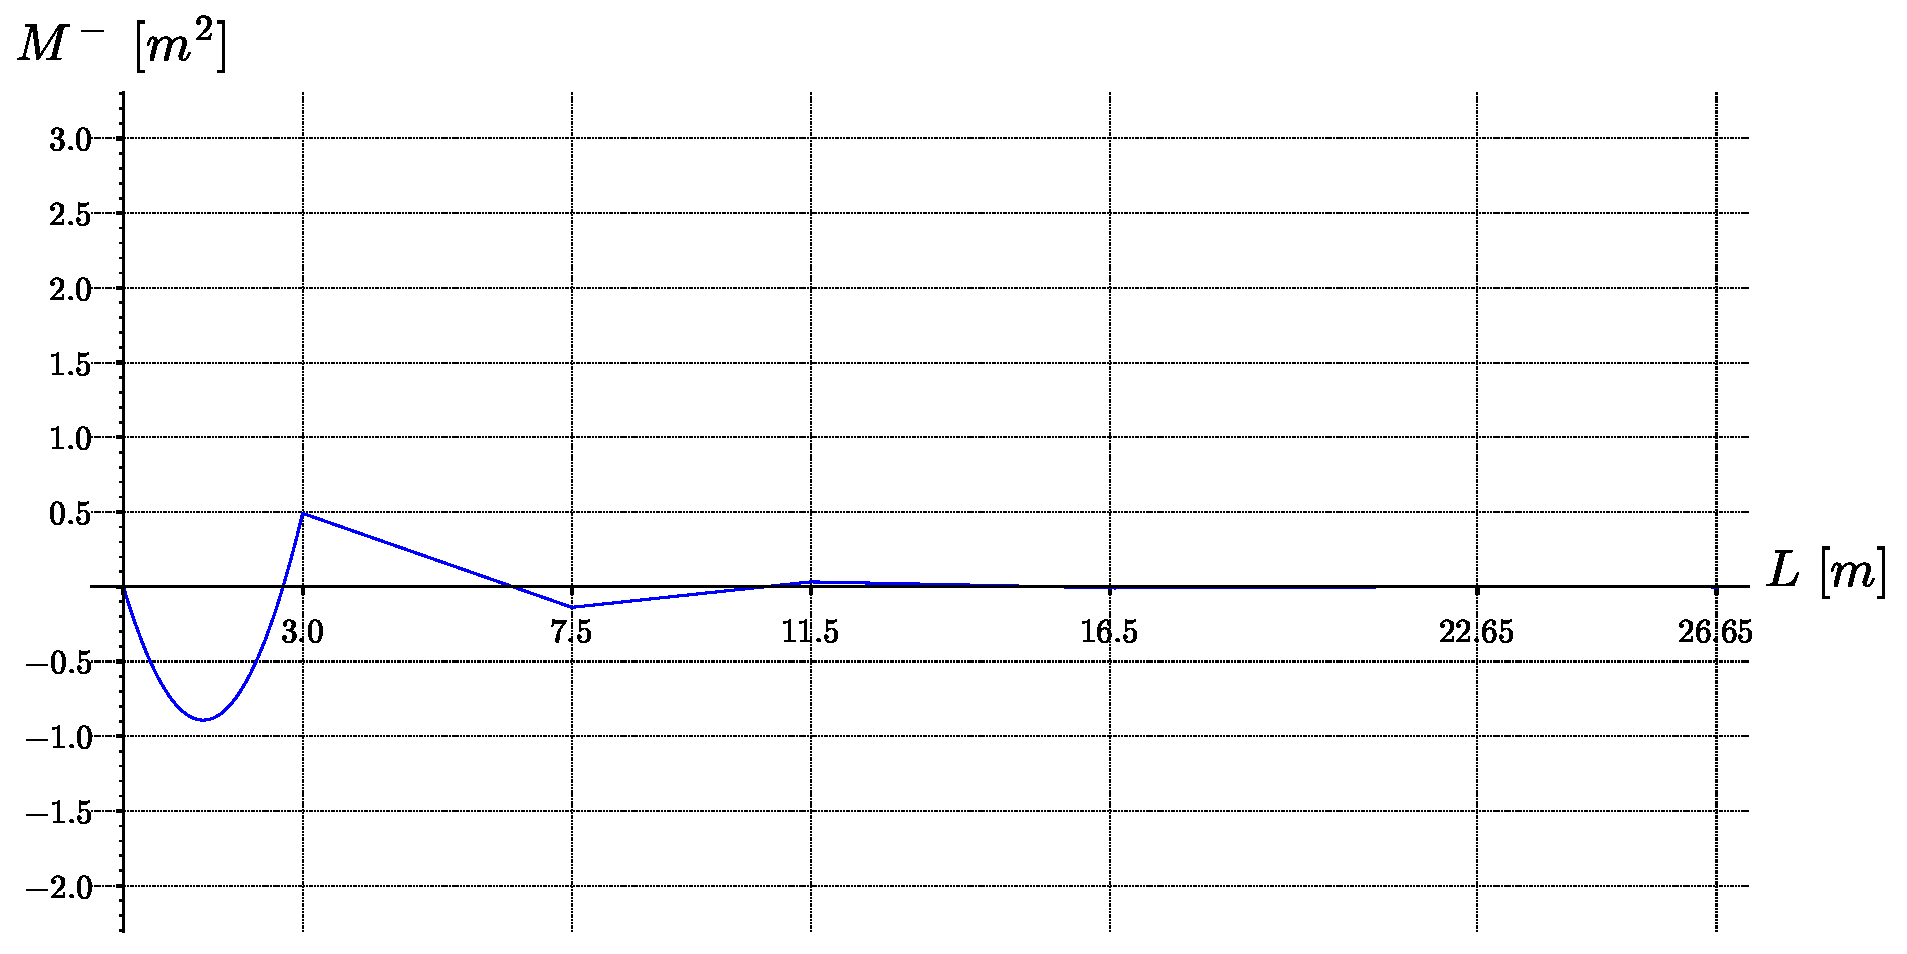
\includegraphics[width=0.45\textwidth]{../imgExportSage/M1_pUnitario.pdf}} \quad
\subfloat[][\emph{Campata 2}]{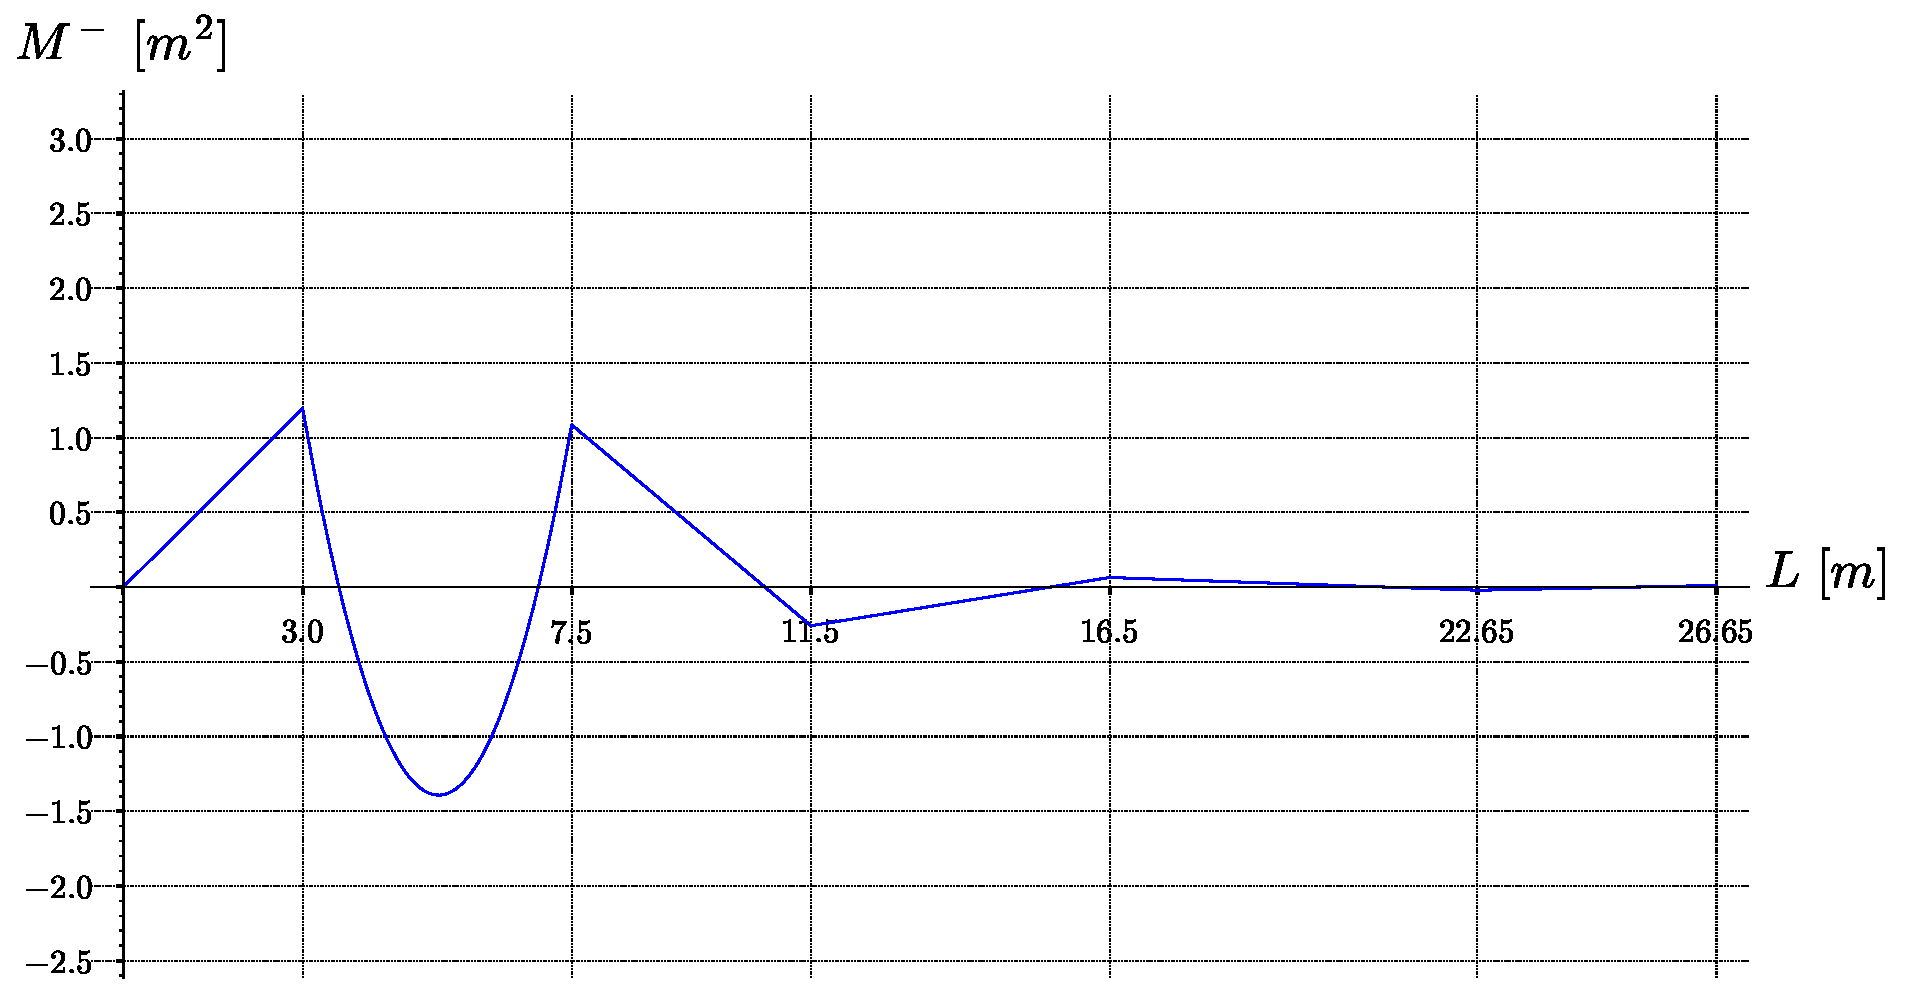
\includegraphics[width=0.45\textwidth]{../imgExportSage/M2_pUnitario}} \\
\subfloat[][\emph{Campata 3}]{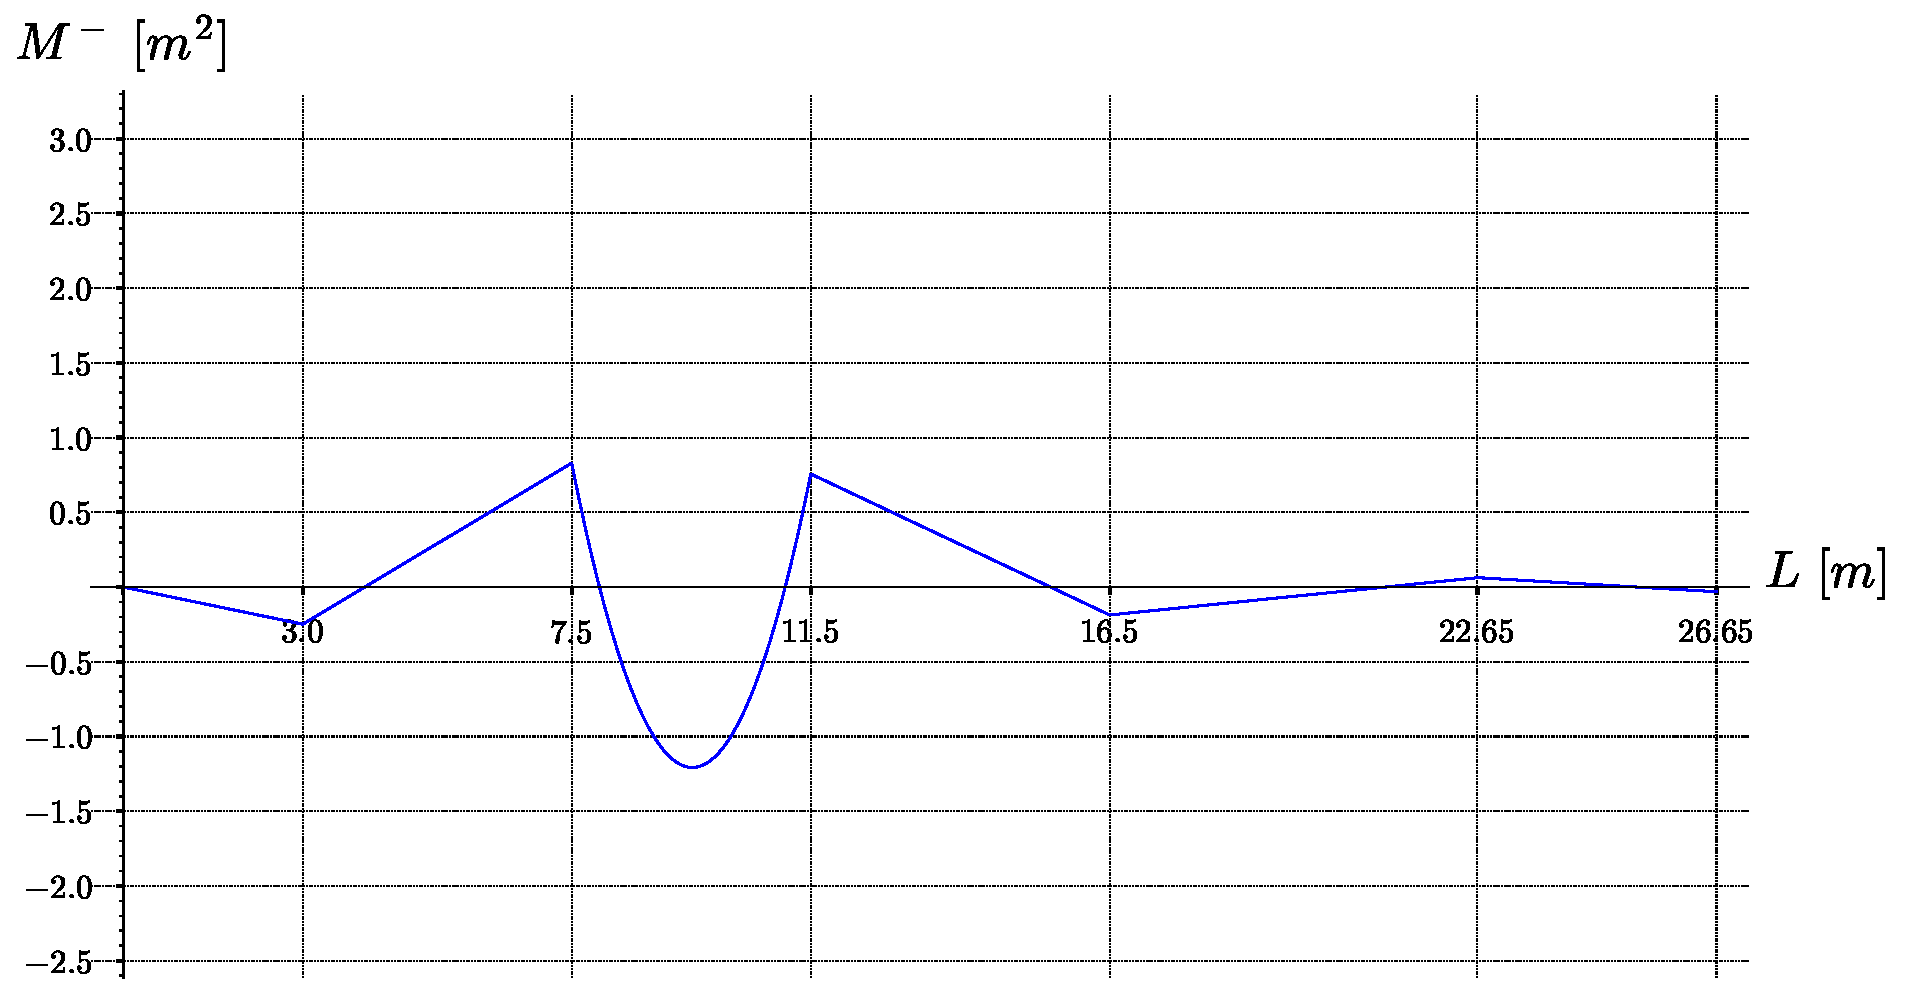
\includegraphics[width=0.45\textwidth]{../imgExportSage/M3_pUnitario}} \quad
\subfloat[][\emph{Campata 4}]{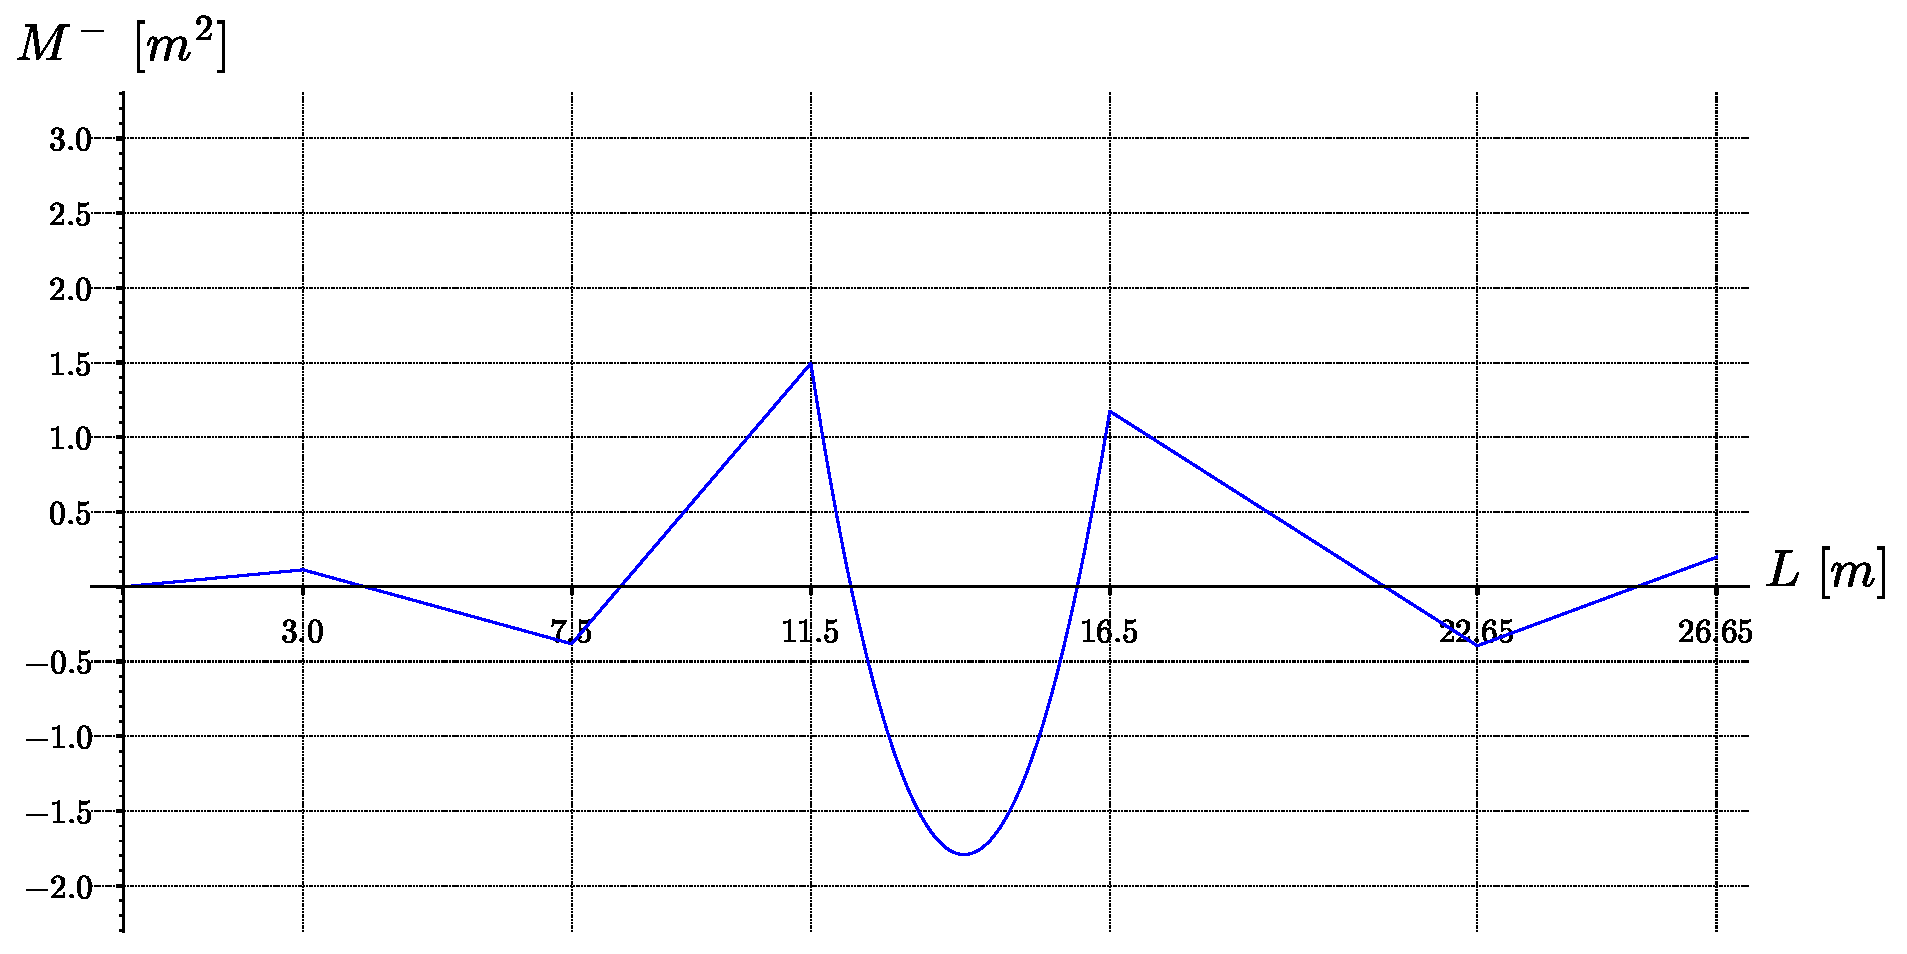
\includegraphics[width=0.45\textwidth]{../imgExportSage/M4_pUnitario}} \\
\subfloat[][\emph{Campata 5}]{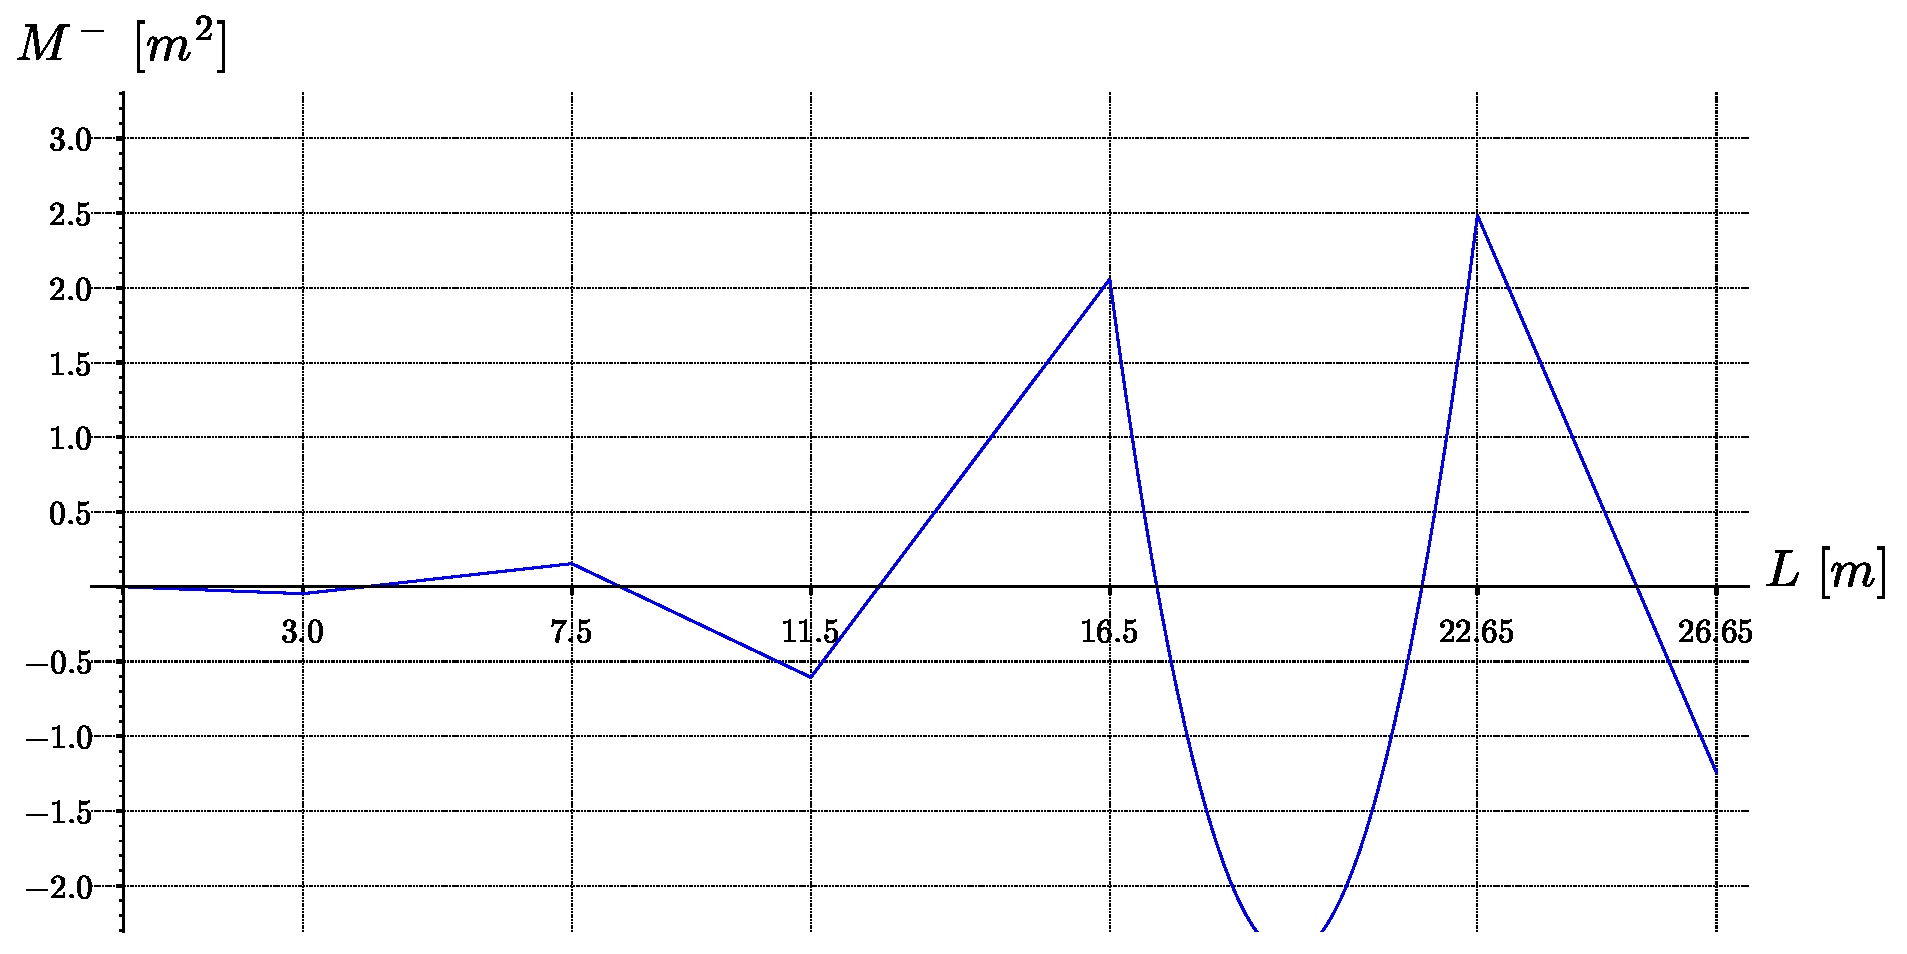
\includegraphics[width=0.45\textwidth]{../imgExportSage/M5_pUnitario.pdf}} \quad
\subfloat[][\emph{Campata 6}]{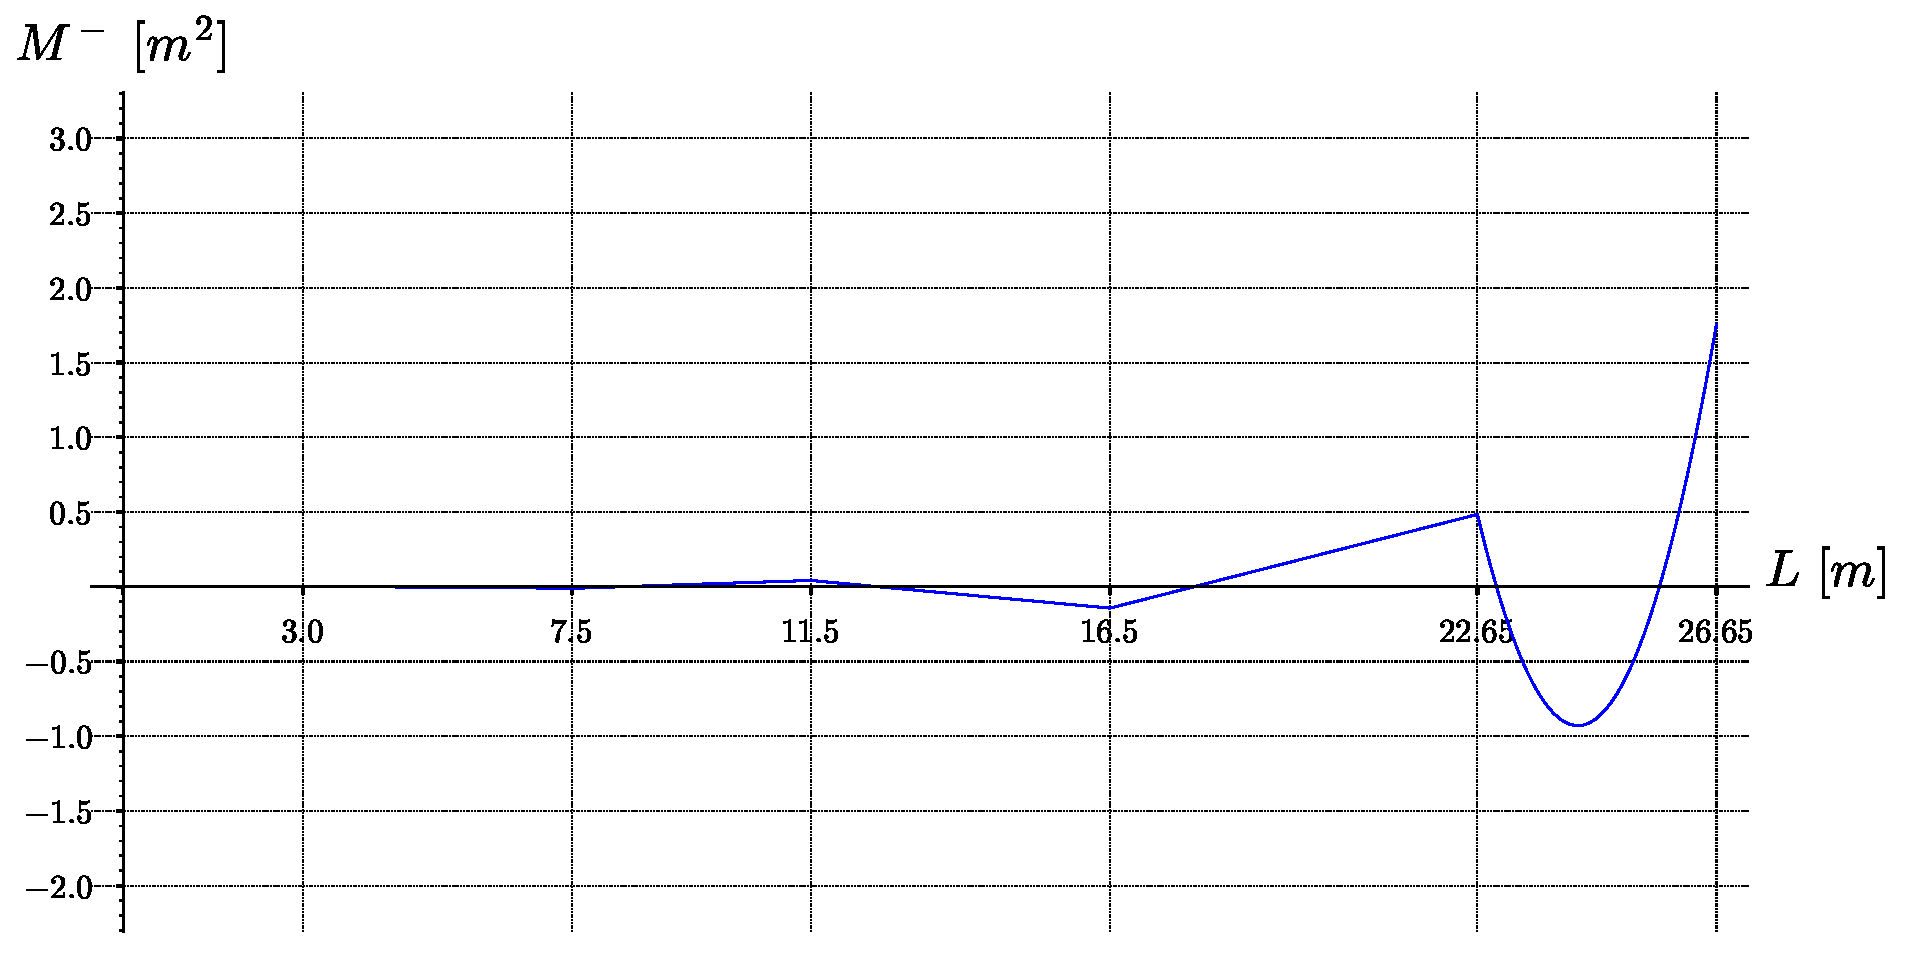
\includegraphics[width=0.45\textwidth]{../imgExportSage/M6_pUnitario}} \\
\subfloat[][\emph{Somma delle campate}]{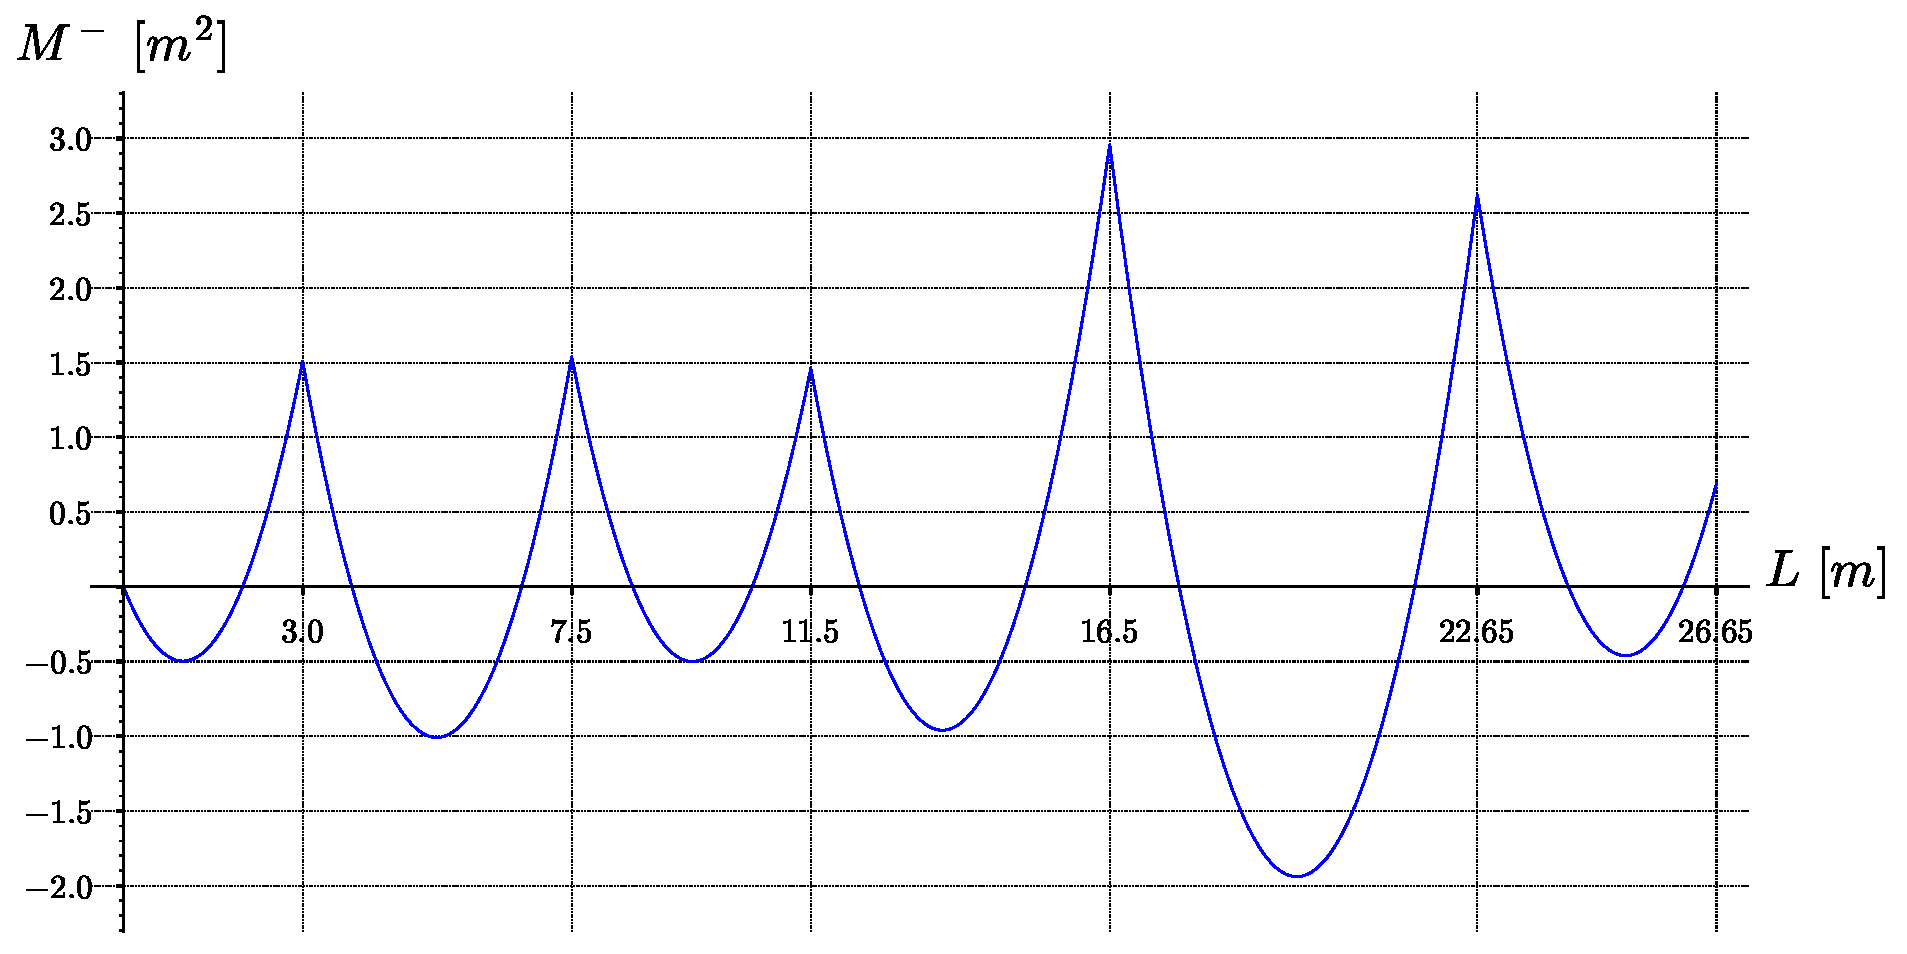
\includegraphics[width=0.6\textwidth]{../imgExportSage/Mtot_pUnitario}}
\caption{Diagrammi dei momenti applicando di volta in volta un carico unitario nelle campate e la somma nel diagramma del momento unitario totale}
\label{fig:MomentiUnitari}
\end{figure}
\section{Taglio unitario}
\begin{figure}[htbp]
\centering
\subfloat[][\emph{Campata 1}]{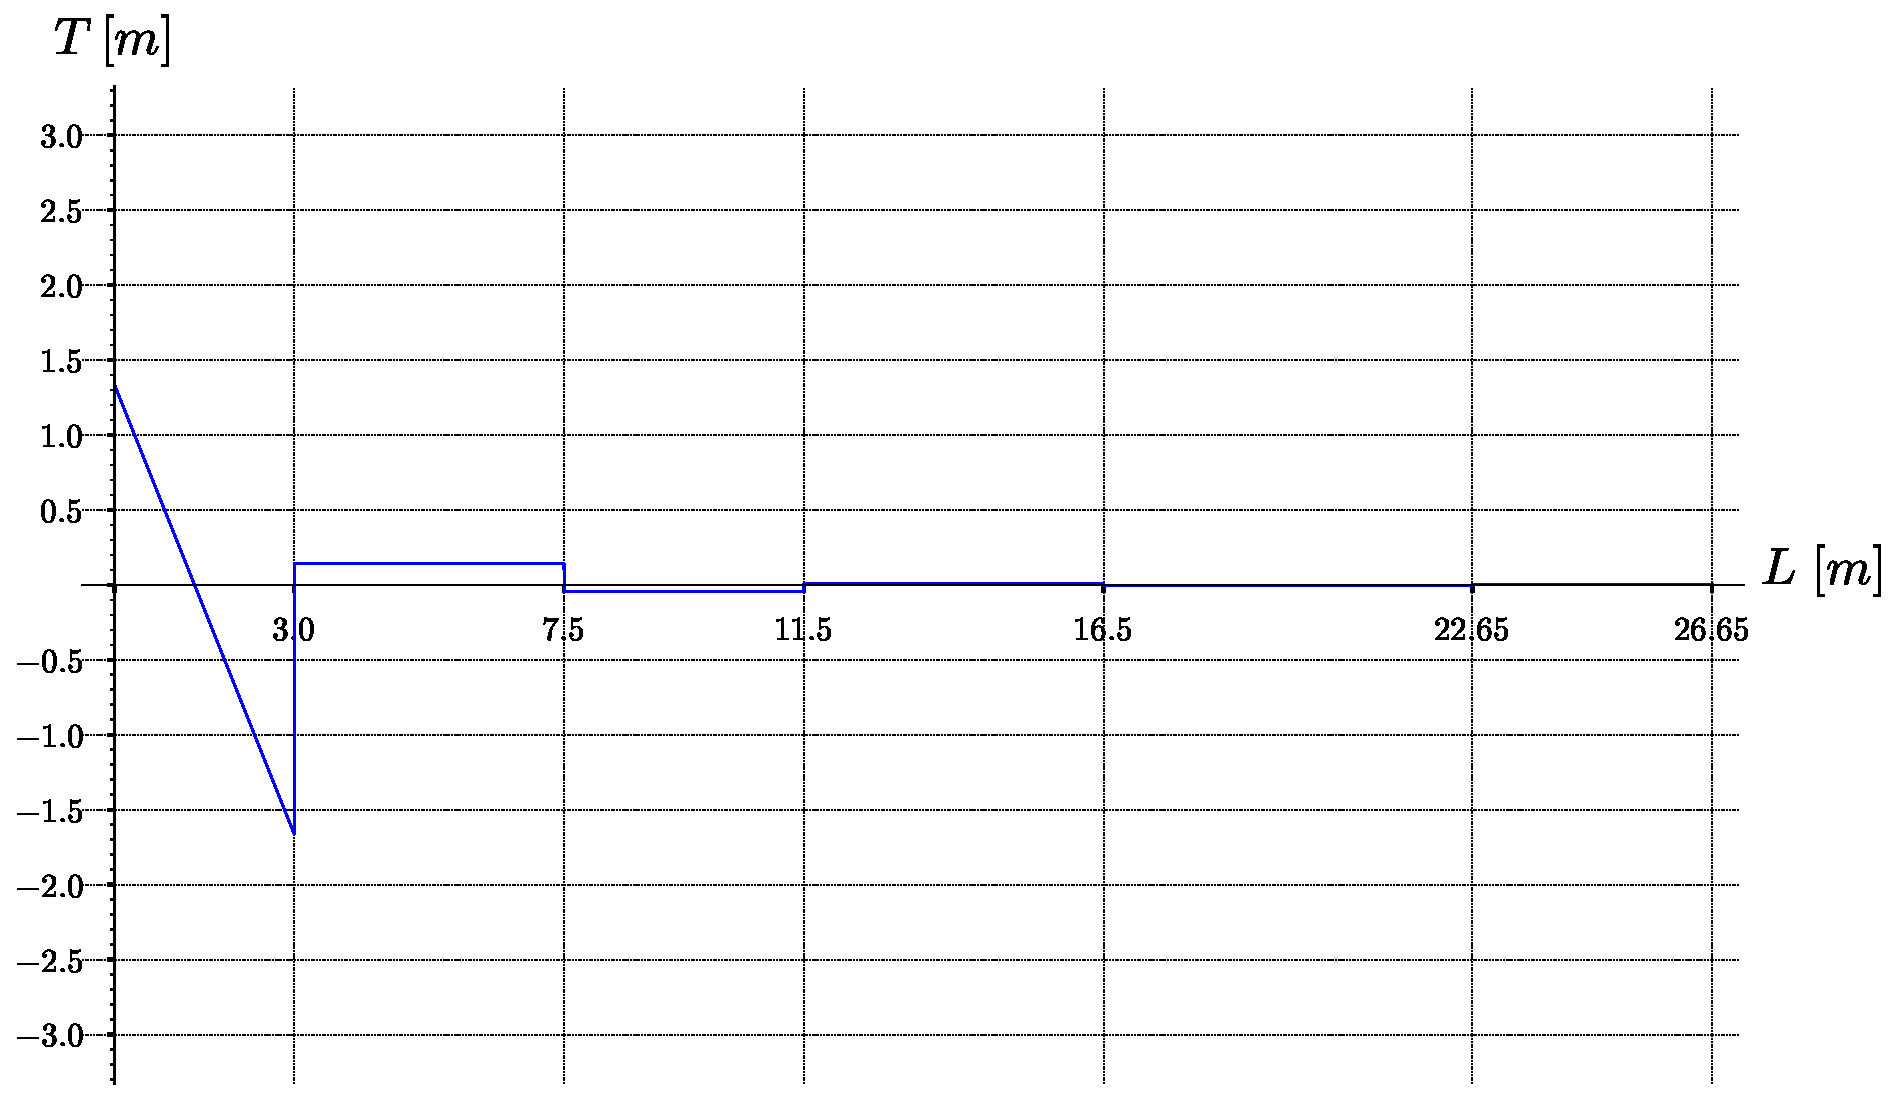
\includegraphics[width=0.45\textwidth]{../imgExportSage/T1_pUnitario.pdf}} \quad
\subfloat[][\emph{Campata 2}]{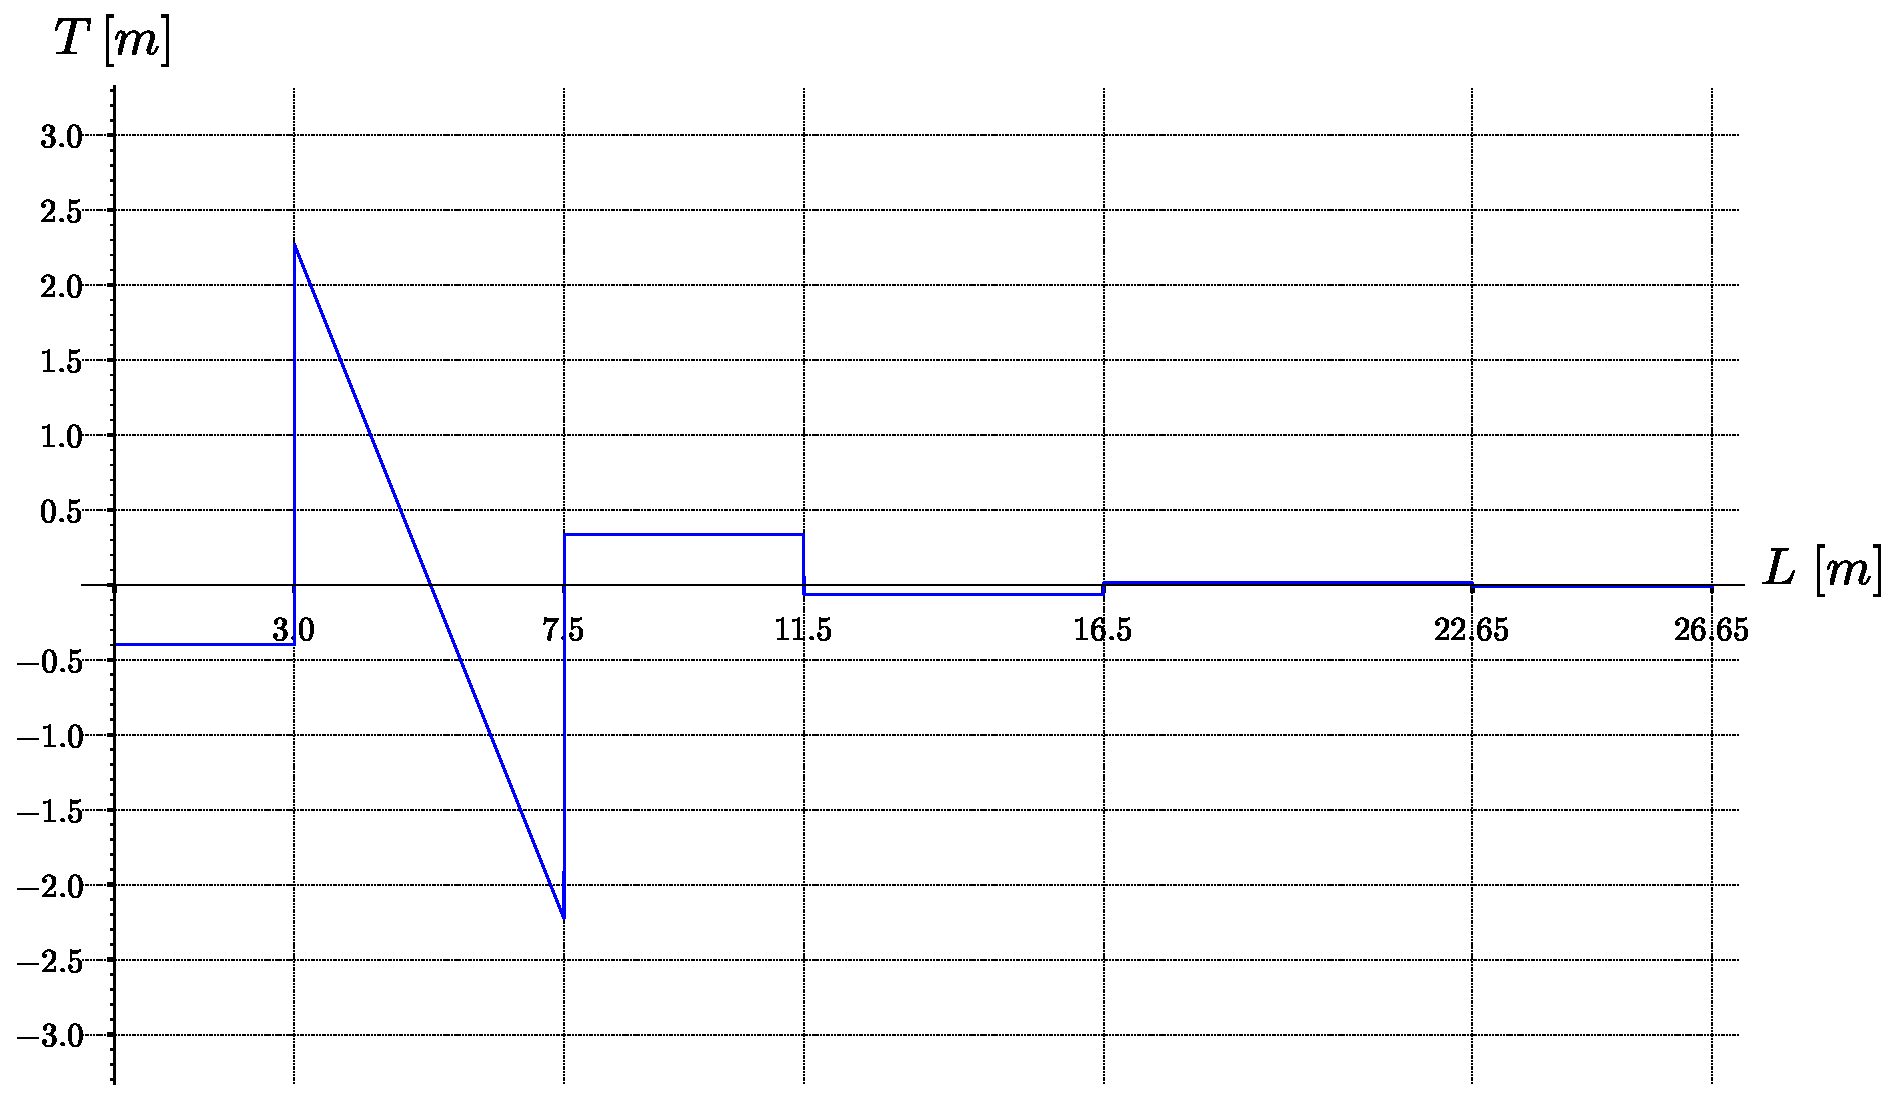
\includegraphics[width=0.45\textwidth]{../imgExportSage/T2_pUnitario}} \\
\subfloat[][\emph{Campata 3}]{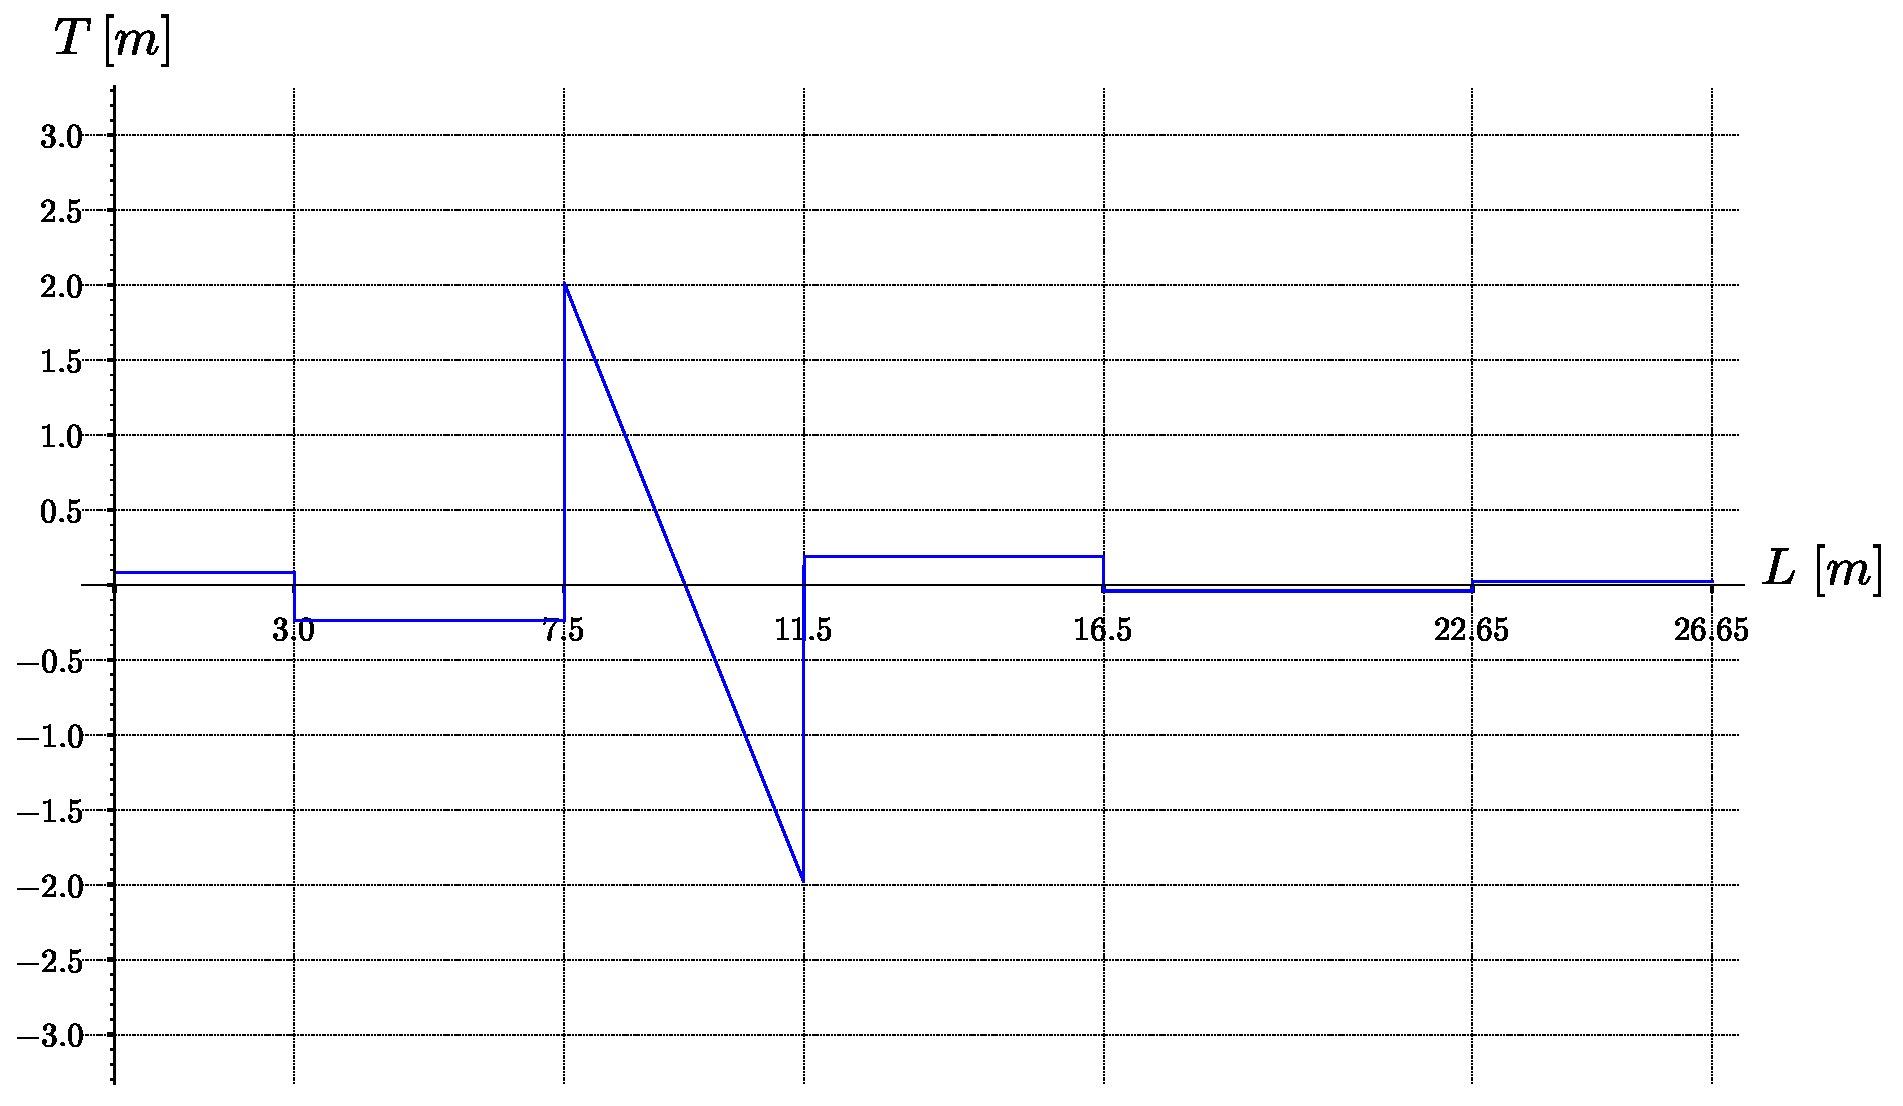
\includegraphics[width=0.45\textwidth]{../imgExportSage/T3_pUnitario}} \quad
\subfloat[][\emph{Campata 4}]{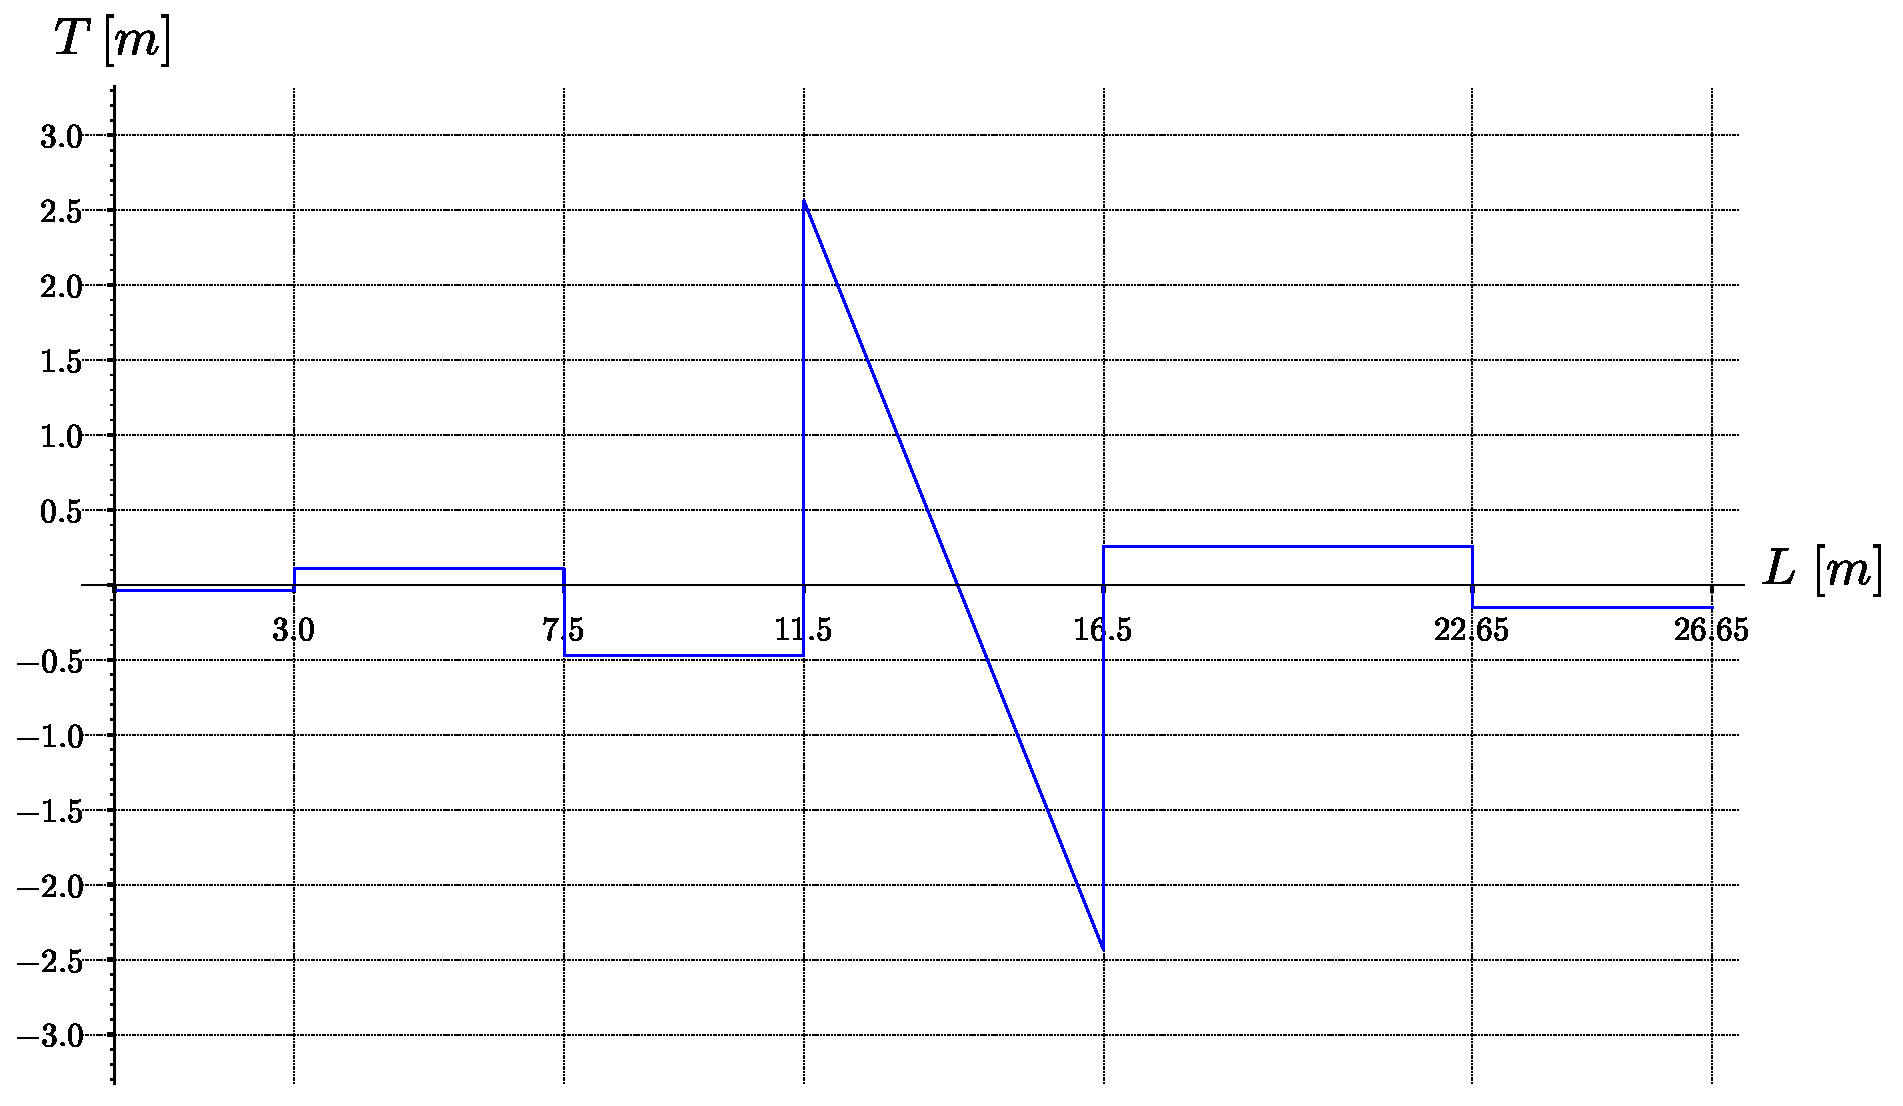
\includegraphics[width=0.45\textwidth]{../imgExportSage/T4_pUnitario}} \\
\subfloat[][\emph{Campata 5}]{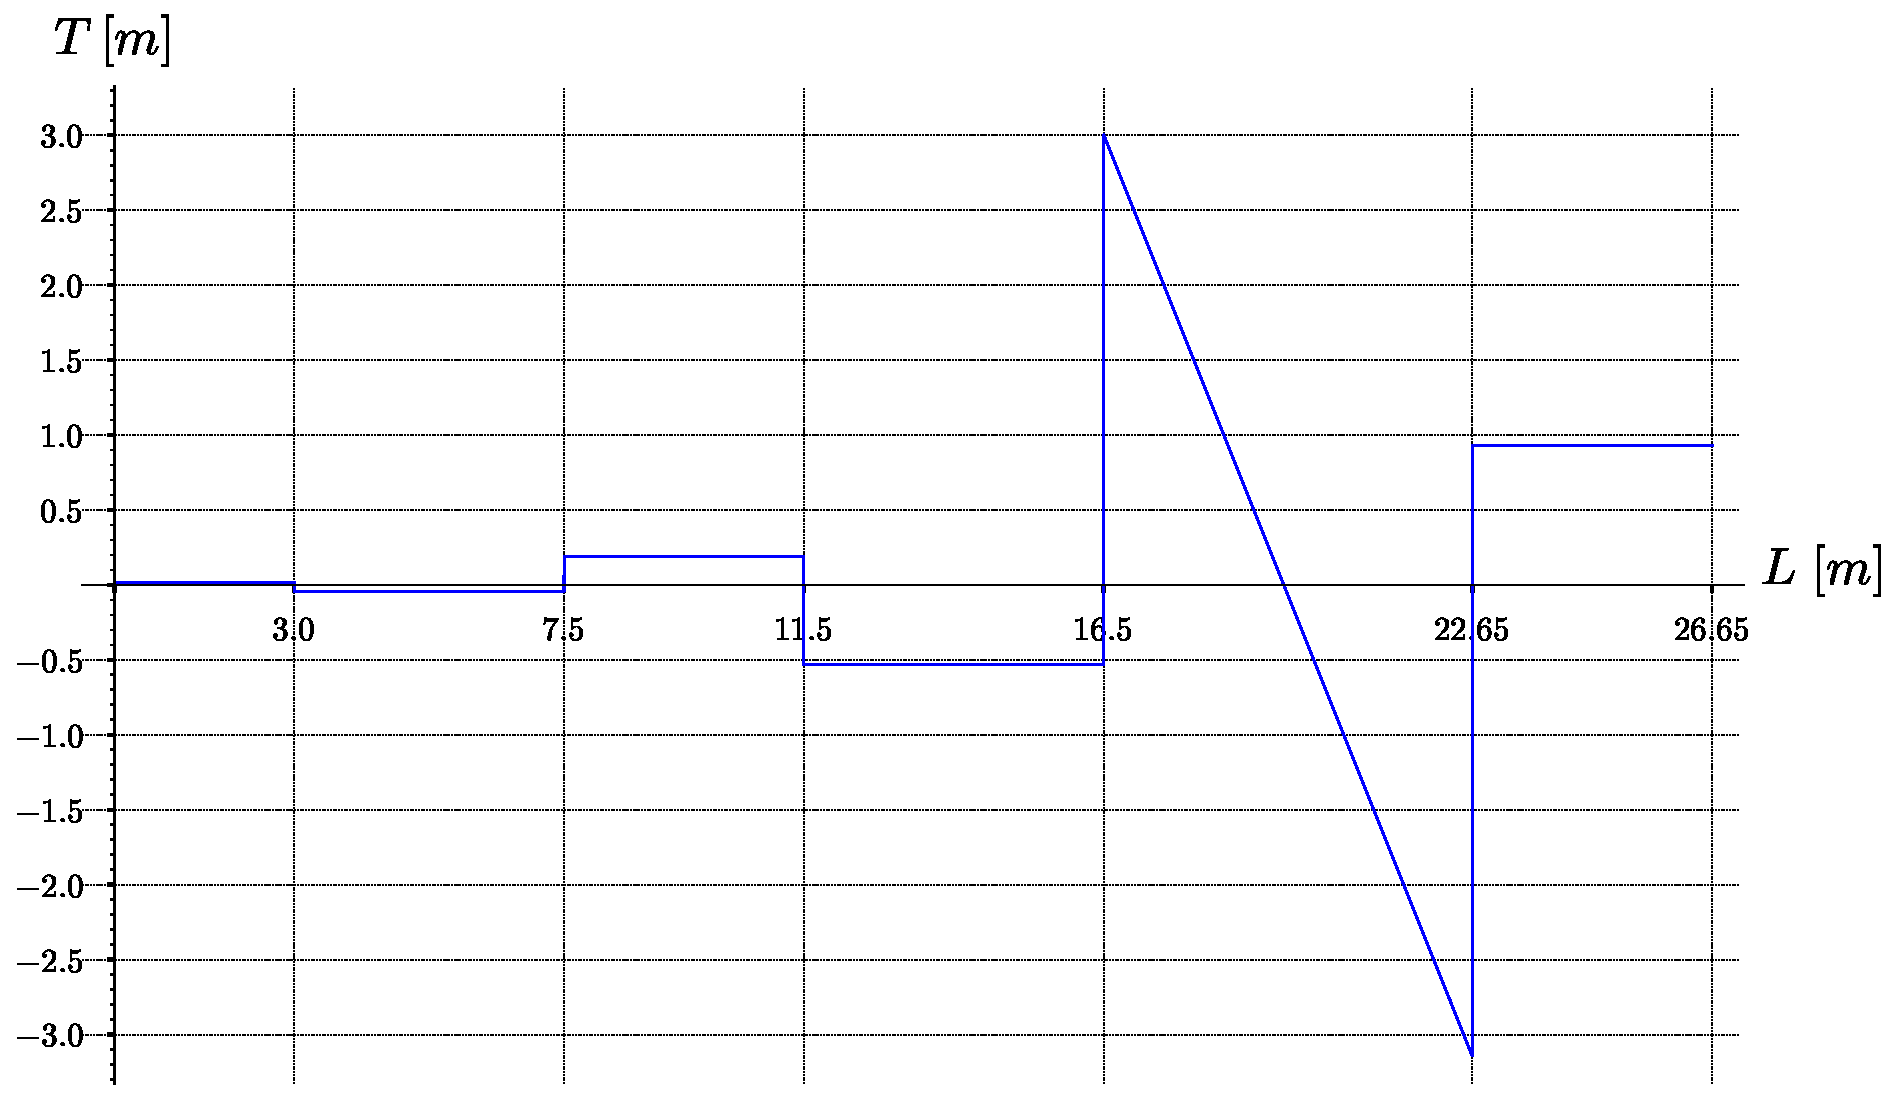
\includegraphics[width=0.45\textwidth]{../imgExportSage/T5_pUnitario.pdf}} \quad
\subfloat[][\emph{Campata 6}]{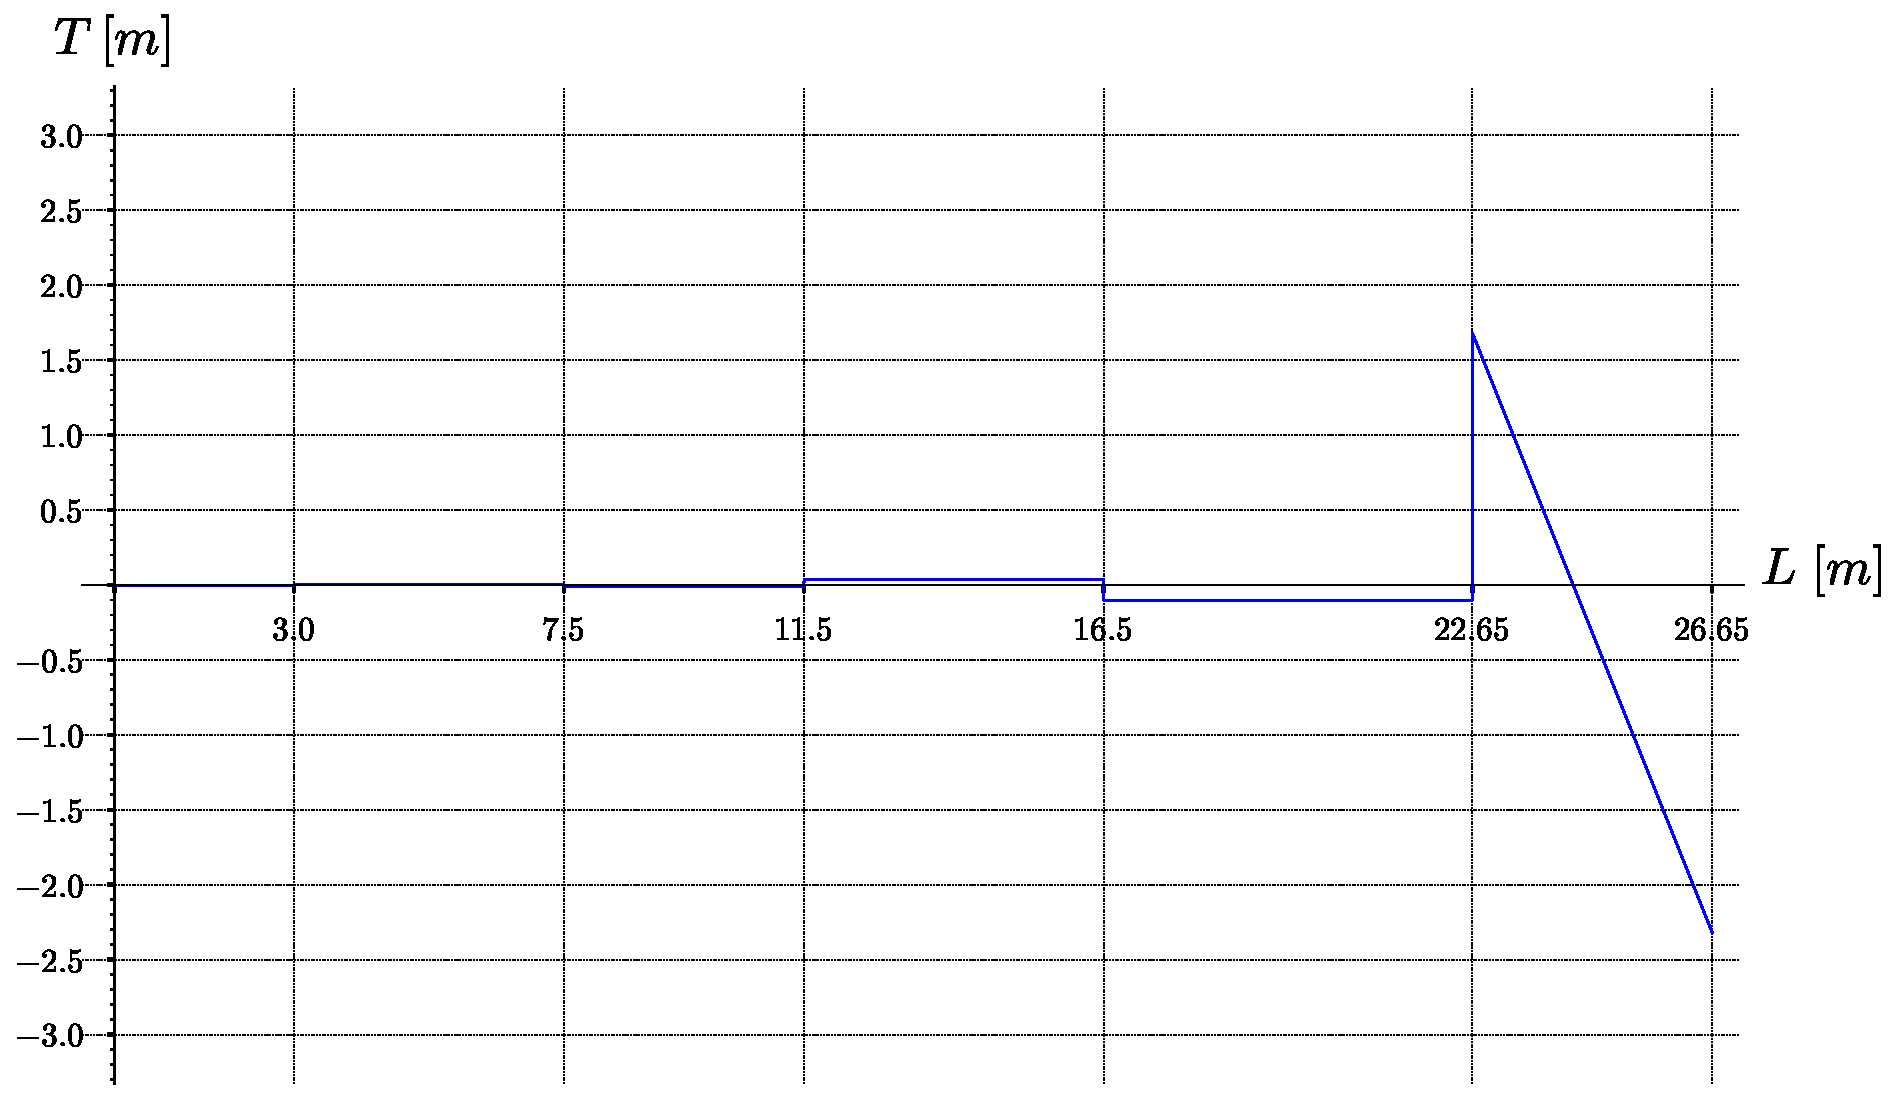
\includegraphics[width=0.45\textwidth]{../imgExportSage/T6_pUnitario}} \\
\subfloat[][\emph{Somma delle campate}]{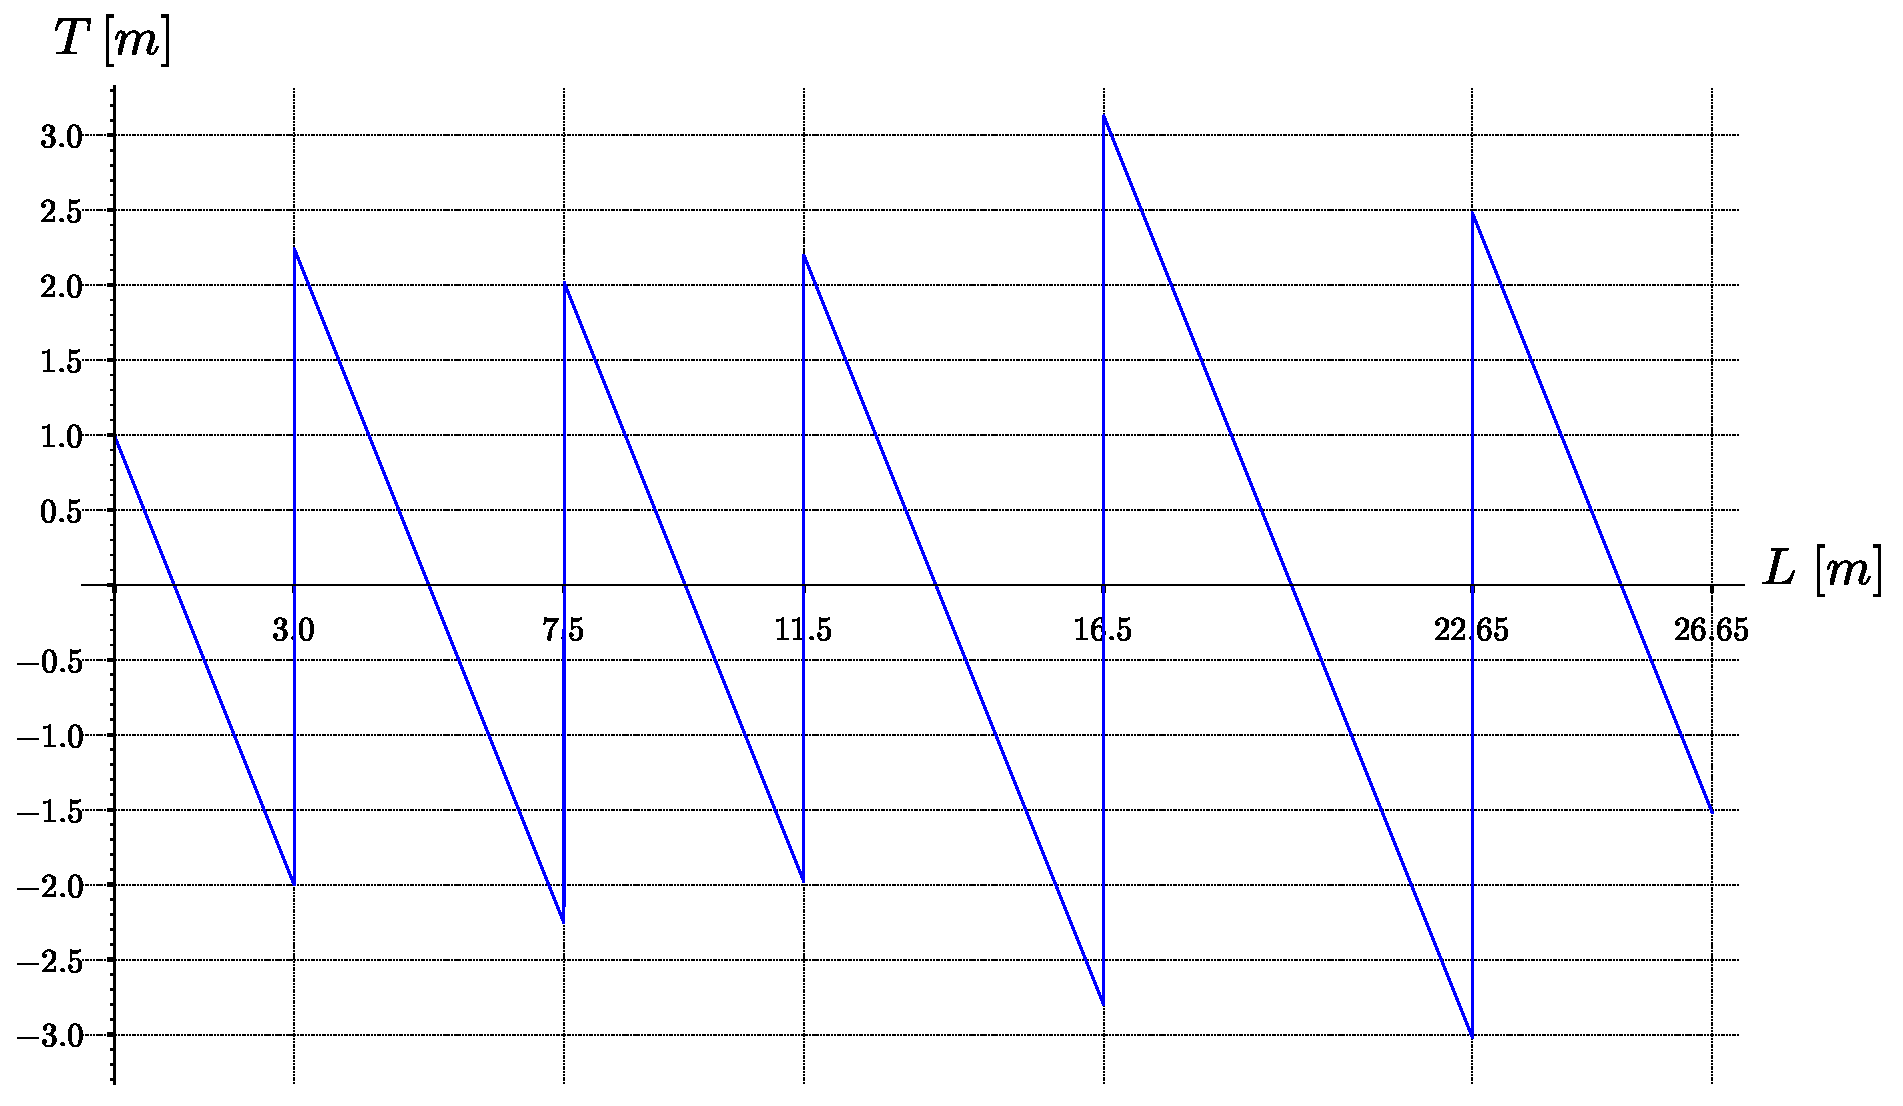
\includegraphics[width=0.6\textwidth]{../imgExportSage/Ttot_pUnitario}}
\caption{Diagrammi del taglio applicando di volta in volta un carico unitario nelle campate e la somma nel diagramma del taglio unitario totale}
\label{fig:TagliUnitari}
\end{figure}
%
\clearpage	
%%%%%%%%%%%%%%%%%%%%%%%%%%%%%%%%%%%%%%
\begin{landscape}
\begin{figure}[H]
\centering
\subfloat[][\emph{Sovrapposizione dei diagrammi del taglio dovuta alle diverse casistiche dei carico illustrate in figura \ref{fig:Struttura2} \label{fig:TagliA_ULS}}]{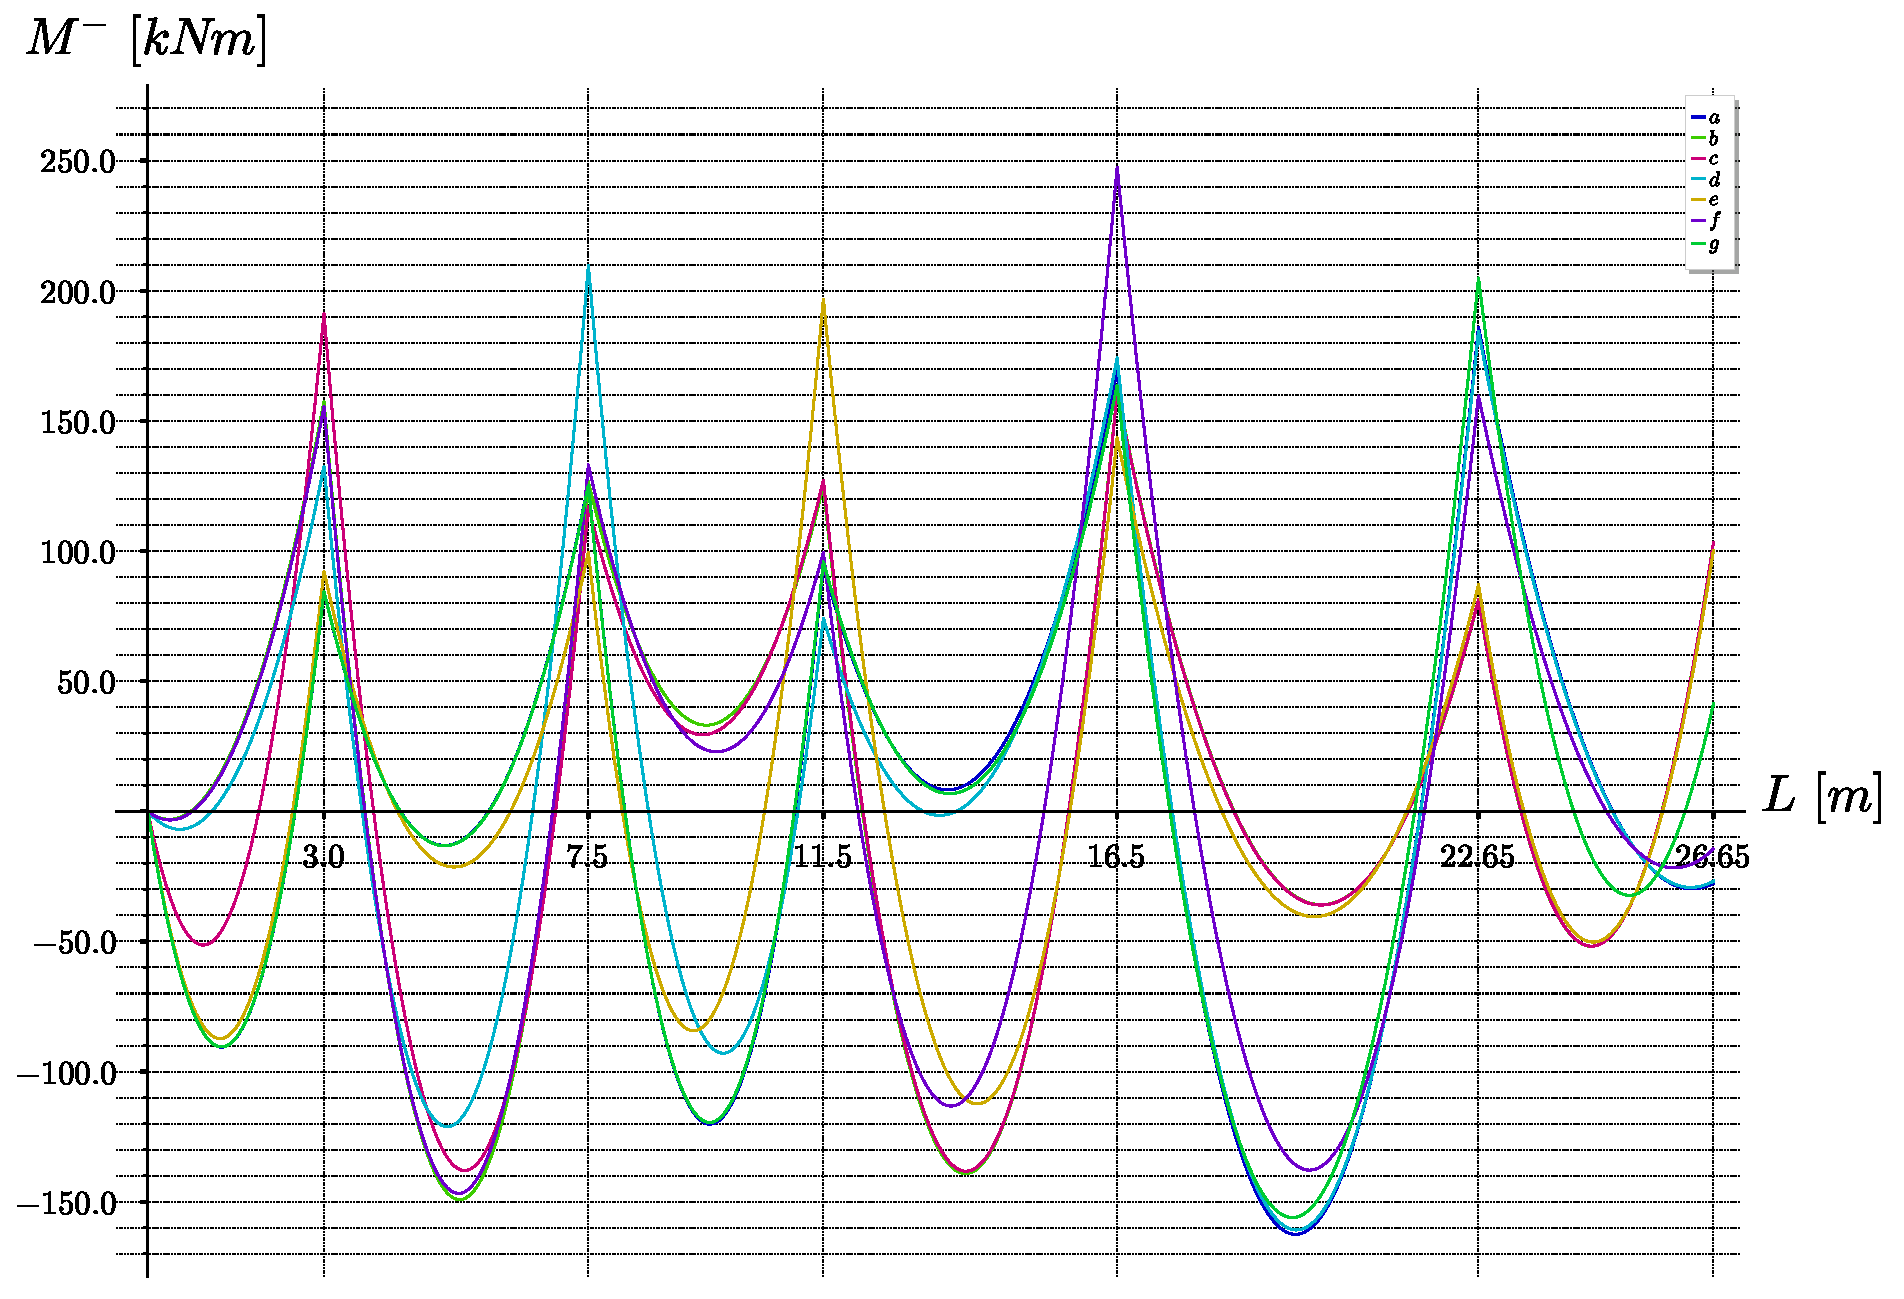
\includegraphics[height=0.5\textwidth]{../imgExportSage/ULS_ptot.pdf}} 
\subfloat[][\emph{Inviluppo dei diagrammi del taglio sovrapposti \label{fig:TagliB_ULS}}]{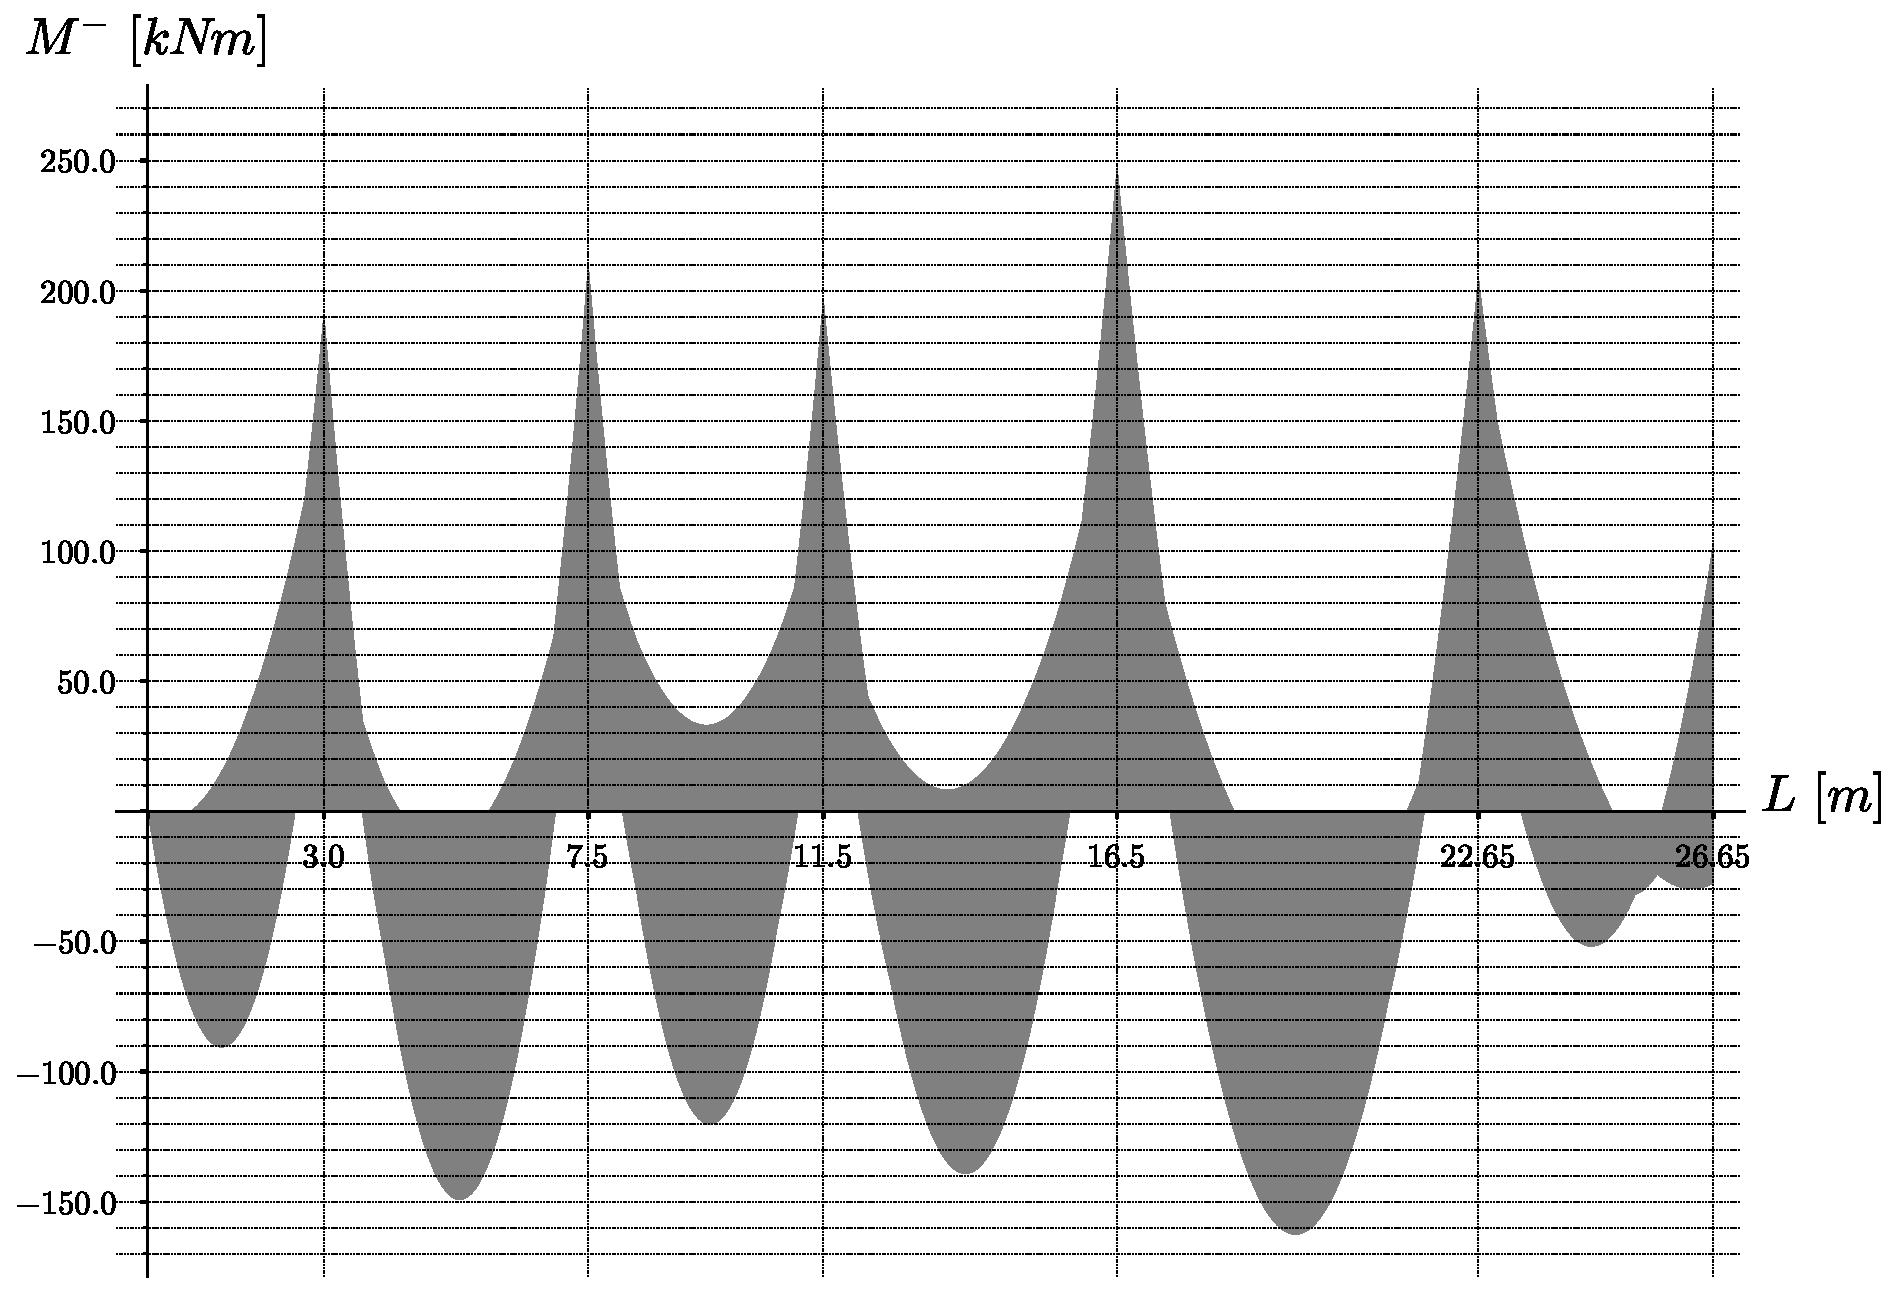
\includegraphics[height=0.5\textwidth]{../imgExportSage/ULS_pInviluppo.pdf}} 
\caption{SLU}
\label{fig:Tagli_ULS}
\end{figure}
\begin{table}[H]
\centering
\caption{boh}
	\begin{tabular}{lS[table-format=3.2]S[table-format=3.2]S[table-format=3.2]S[table-format=3.2]S[table-format=3.2]S[table-format=3.2]S[table-format=3.2]S[table-format=3.2]S[table-format=3.2]S[table-format=3.2]S[table-format=3.2]S[table-format=3.2]S[table-format=3.2]}
		\toprule
		&\multicolumn{1}{c}{N1}&\multicolumn{1}{c}{N1}&\multicolumn{1}{c}{N1}&\multicolumn{1}{c}{N1}&\multicolumn{1}{c}{N1}&\multicolumn{1}{c}{N1}&\multicolumn{1}{c}{N1}&\multicolumn{1}{c}{N1}&\multicolumn{1}{c}{N1}&\multicolumn{1}{c}{N1}&\multicolumn{1}{c}{N1}&\multicolumn{1}{c}{N1}&\multicolumn{1}{c}{N1}\\
		\midrule
		$M^{-}$&999.99&999.99&999.99&999.99&999.99&999.99&999.99&999.99&999.99&999.99&999.99&999.99&999.99\\
		$M^{+}$&999.99&999.99&999.99&999.99&999.99&999.99&999.99&999.99&999.99&999.99&999.99&999.99&999.99\\
		\bottomrule
	\end{tabular}
\end{table}
\end{landscape}
\clearpage
\begin{landscape}
\begin{figure}[H]
\centering
\subfloat[][\emph{Sovrapposizione dei diagrammi del taglio dovuta alle diverse casistiche dei carico illustrate in figura \ref{fig:Struttura2} \label{fig:TagliA_ULS}}]{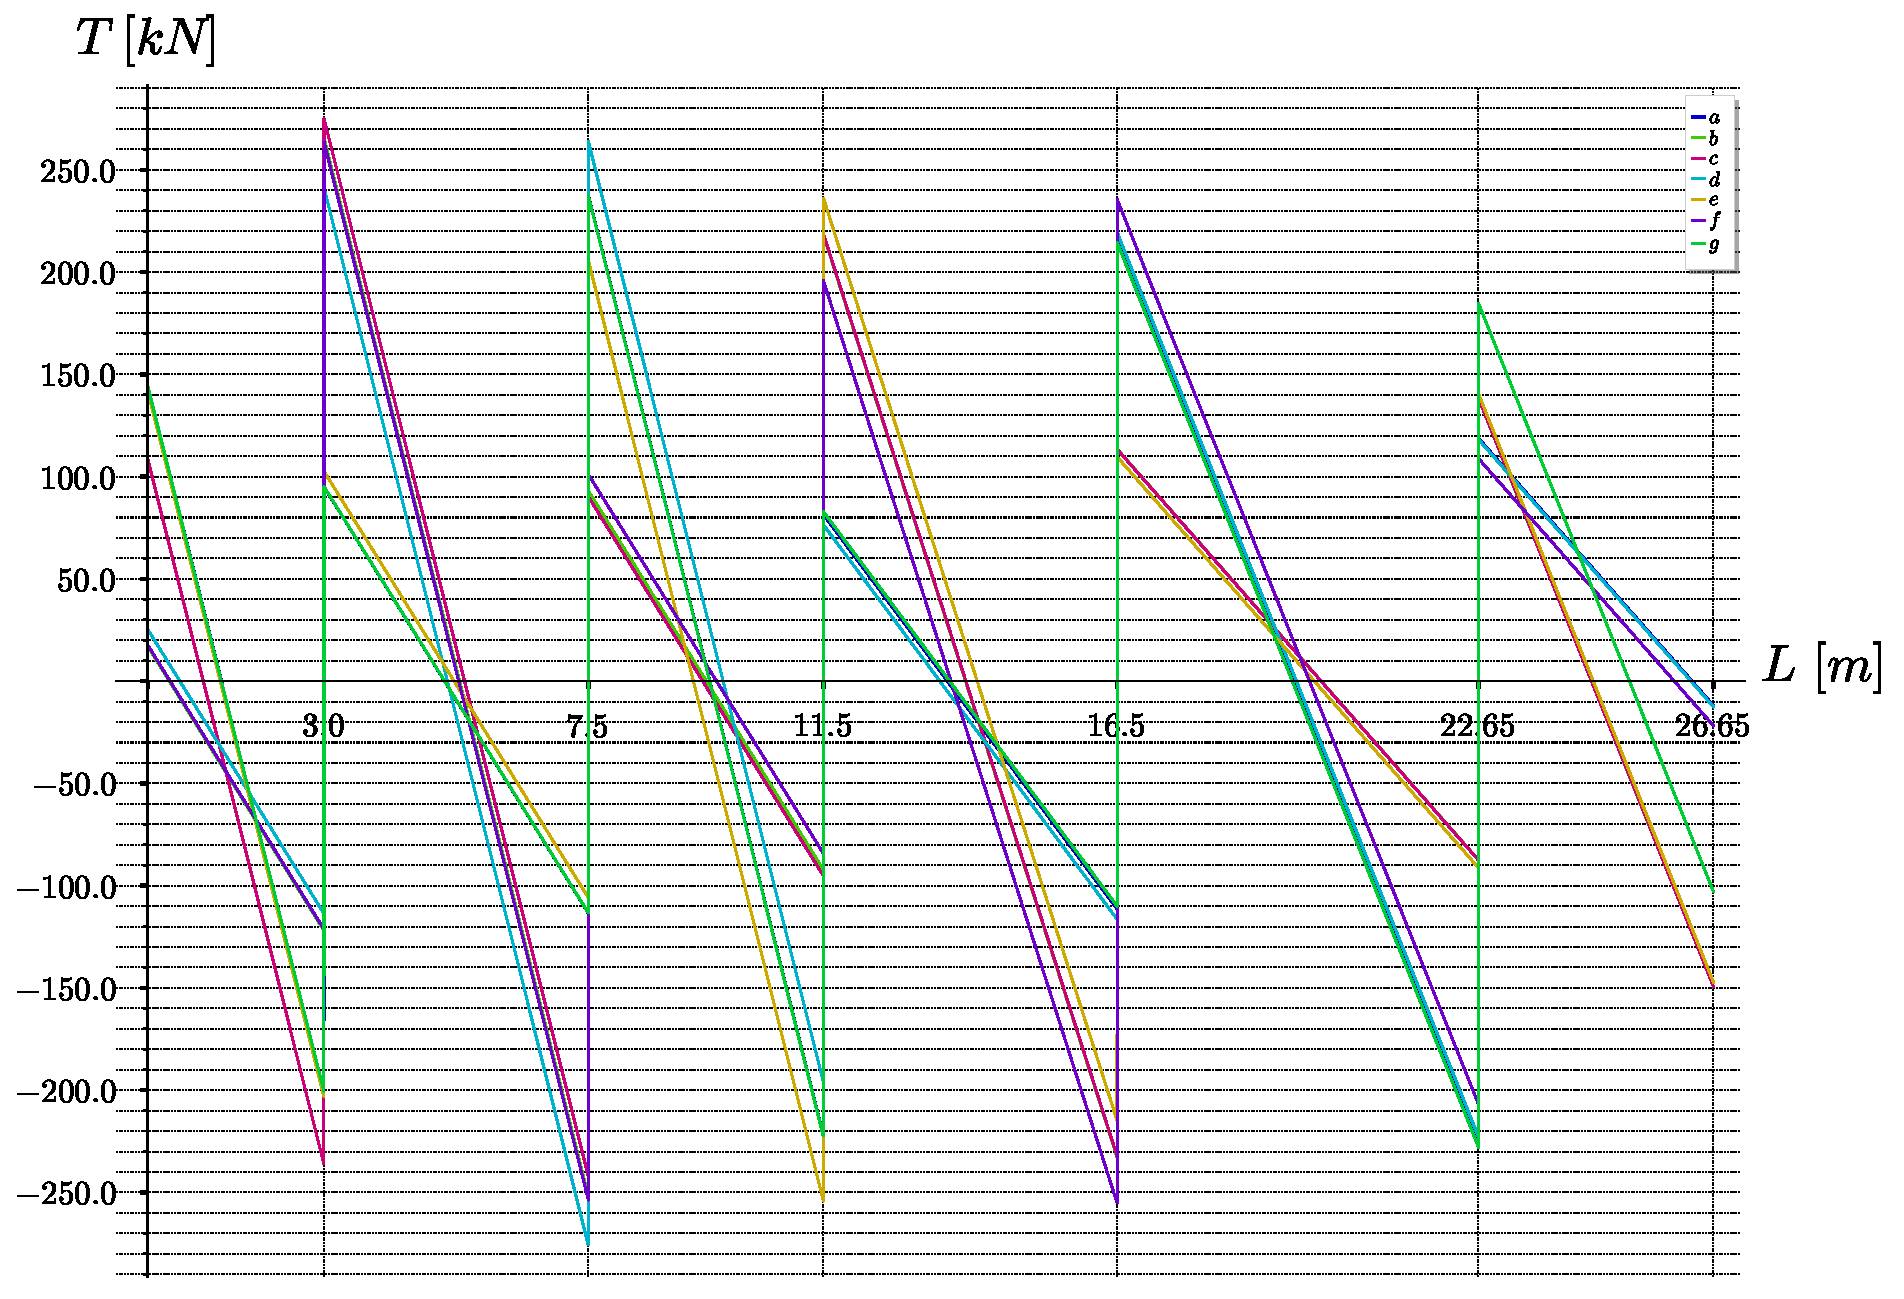
\includegraphics[height=0.5\textwidth]{../imgExportSage/ULS_Tptot.pdf}} 
\subfloat[][\emph{Inviluppo dei diagrammi del taglio sovrapposti \label{fig:TagliB_ULS}}]{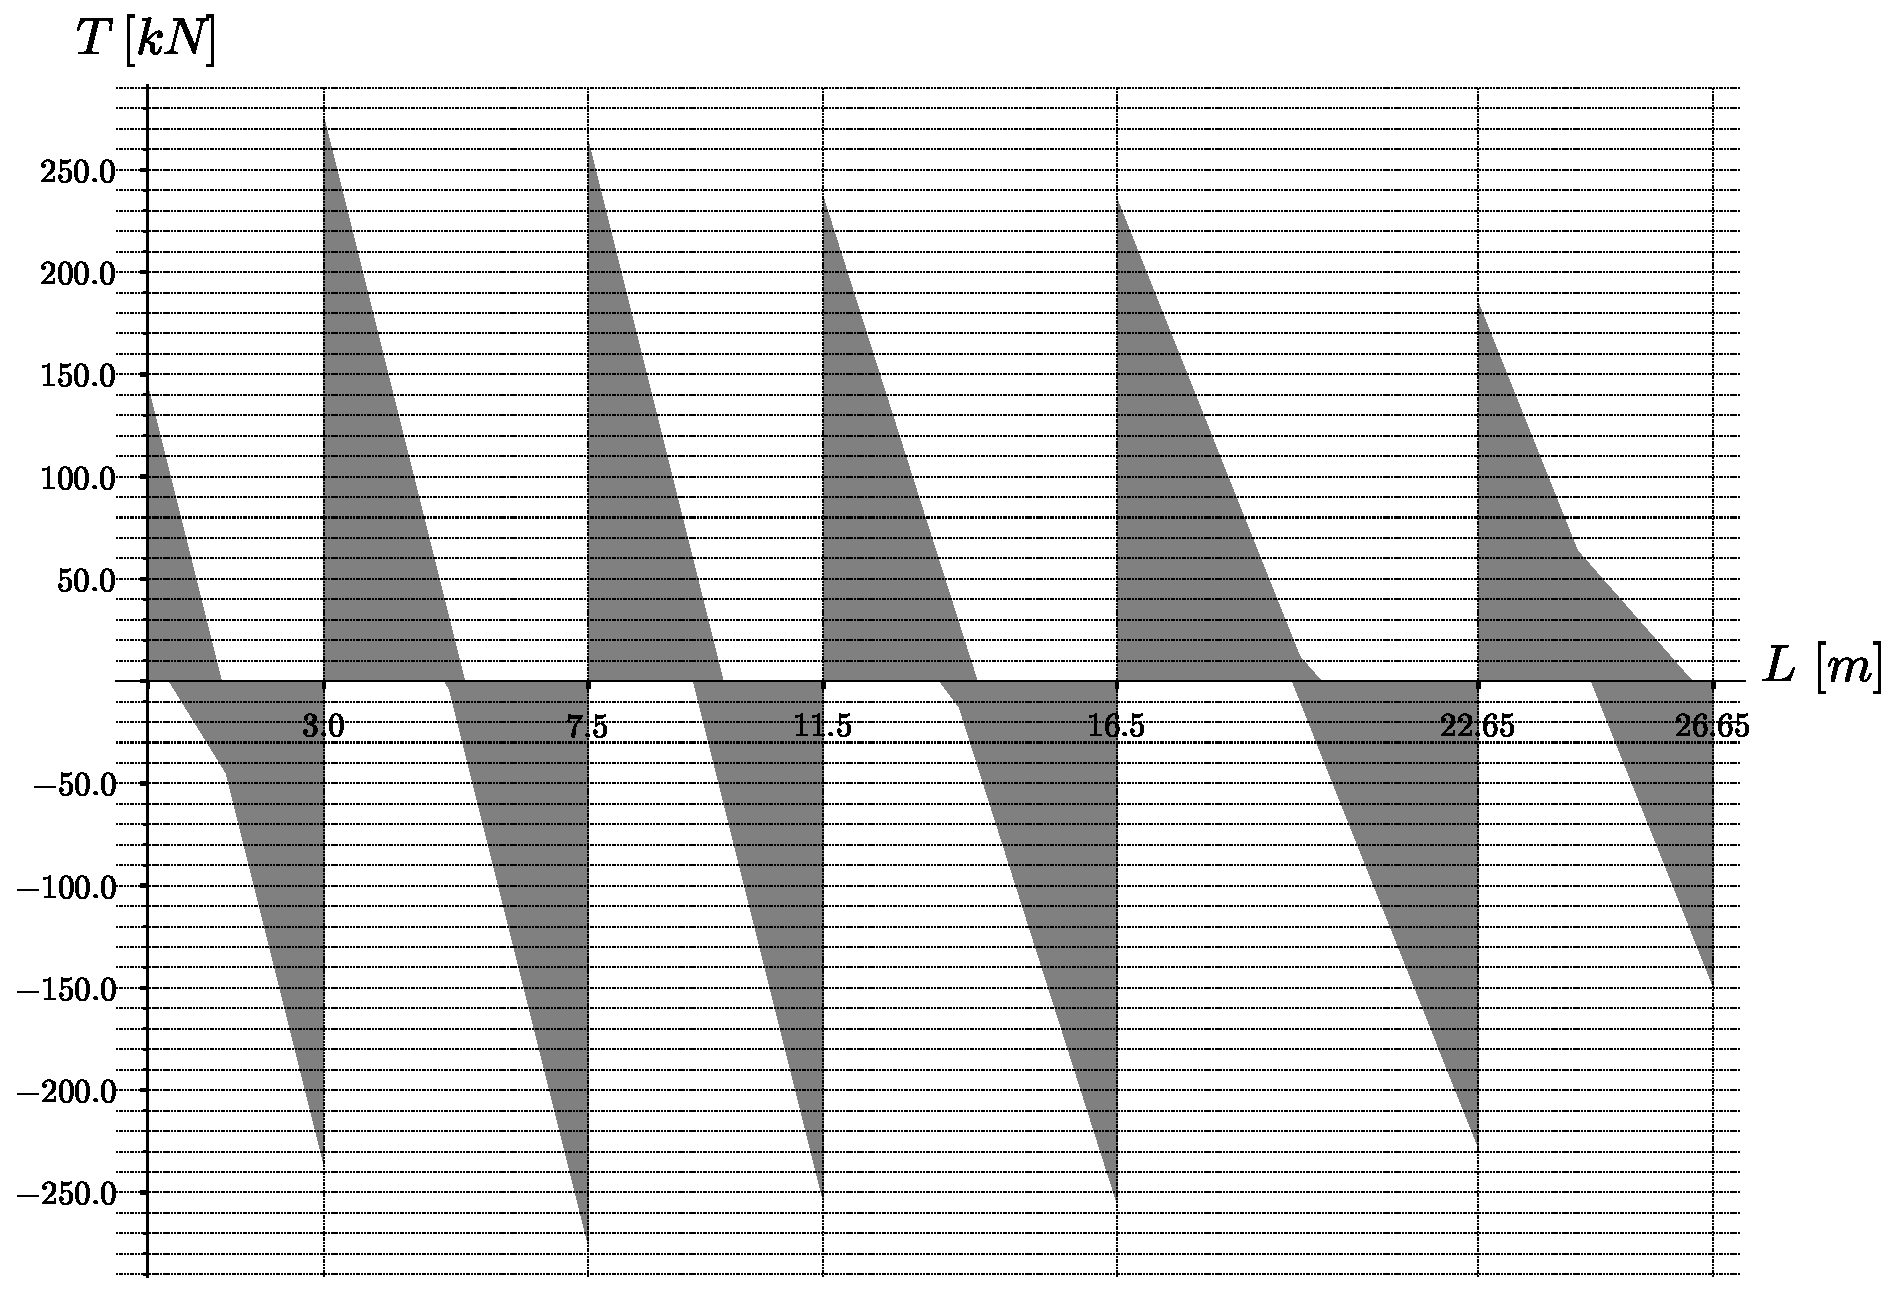
\includegraphics[height=0.5\textwidth]{../imgExportSage/ULS_TpInviluppo.pdf}} 
\caption{SLU}
\label{fig:Tagli_ULS}
\end{figure}
\begin{table}[H]
\centering
\caption{boh}
	\begin{tabular}{lS[table-format=3.2]S[table-format=3.2]S[table-format=3.2]S[table-format=3.2]S[table-format=3.2]S[table-format=3.2]S[table-format=3.2]S[table-format=3.2]S[table-format=3.2]S[table-format=3.2]S[table-format=3.2]S[table-format=3.2]S[table-format=3.2]}
		\toprule
		&\multicolumn{1}{c}{N1}&\multicolumn{1}{c}{N1}&\multicolumn{1}{c}{N1}&\multicolumn{1}{c}{N1}&\multicolumn{1}{c}{N1}&\multicolumn{1}{c}{N1}&\multicolumn{1}{c}{N1}&\multicolumn{1}{c}{N1}&\multicolumn{1}{c}{N1}&\multicolumn{1}{c}{N1}&\multicolumn{1}{c}{N1}&\multicolumn{1}{c}{N1}&\multicolumn{1}{c}{N1}\\
		\midrule
		$M^{-}$&999.99&999.99&999.99&999.99&999.99&999.99&999.99&999.99&999.99&999.99&999.99&999.99&999.99\\
		$M^{+}$&999.99&999.99&999.99&999.99&999.99&999.99&999.99&999.99&999.99&999.99&999.99&999.99&999.99\\
		\bottomrule
	\end{tabular}
\end{table}
\end{landscape}
%!TEX root = ../RelazioneStrutturaleMeoliNicola.tex
\chapter{Pilastro P27}
Si vede ora il calcolo dello sforzo normale per il pilastro P27, analizzando i carichi agenti nei vari piani ed elencate le aree di influenza operanti su tale pilastro. 

Nella suddivisione dei piani adottata si intende in riferimento all'intradosso del piano in questione a cui è compreso il contributo del pilastro sopra.

Il peso proprio è calcolato considerando un peso specifico $\gamma_{CLS}$ pari a \SI{25.0}{\kilo\newton\per\meter\cubed} moltiplicato per i lati di \SI{30}{\centi\meter} e le altezze di interpiano riportate nella sezione.
\section{Analisi dei carichi}
Si ha a che fare con un pilastro interno perciò come carico variabile nei solai interni si ha soltanto quello della propria categoria. 
In copertura si ha in aggiunta il carico della neve e del vento.
\subsection{Piano terra}
\paragraph*{G1} \e presente il solaio a lastre Predalle con peso ultimato pari a $g_1^{PT}=\SI{3.60}{\kilo\newton\per\square\meter}$
\paragraph*{G2} \e presente lo stesso solaio visto nel paragrafo a pagina \pageref{cap:g2Trave} con la differenza che l'altezza di interpiano di \SI{3.50}{\meter} è tale per cui occorre considerare un carico distribuito per le pareti interne pari a \SI{1.60}{\kilo\newton\per\square\meter}. 
Si ottiene pertanto
\begin{center}
\begin{tabular}{lS[table-format=2.1]S[table-format=1.2]S[table-format=1.3]}
	\toprule
	\multirow{2}{*}{Strato} & \multicolumn{1}{c}{Peso specifico} & \multicolumn{1}{c}{Spessore}& \multicolumn{1}{c}{$g_{2,k}$}\\
    	   & \multicolumn{1}{c}{$\left[\SI{}{\kilo\newton\per\meter\cubed}\right]$} & \multicolumn{1}{c}{$\left[\SI{}{\meter}\right]$}& \multicolumn{1}{c}{$\left[\SI{}{\kilo\newton\per\square\meter}\right]$}\\
	\midrule
	Sottofondo CLS alleggerito 	 & 16.0 & 0.08 & 1.28 \\
	Massetto allettamento 	     & 24.0 & 0.06 & 1.44 \\
	Pavimento ceramica 	         &      &      & 0.50 \\
	Intonaco intradosso 	     & 20.0 & 0.01 & 0.20 \\
	Pareti interne distribuite   &      &      & 1.60 \\
	\midrule
	Totale $g_2^{PT} =$          &      &      & 5.02 \\
	\bottomrule
\end{tabular}
\end{center}
\paragraph*{Categoria D1 - Negozi} La \normaref{Tab.\,3.1.II} prevede un carico di \SI{4.00}{\kilo\newton\per\square\meter} per la categoria negozi.
\subsection{Piano primo} Sono presenti gli stessi carichi visti per la trave nella parte di solaio interno. 
Ovvero:
\begin{align*}
g_1^{P1} &= \SI{3.20}{\kilo\newton\per\square\meter}\\
g_2^{P1} &= \SI{4.62}{\kilo\newton\per\square\meter}\\
q_{cat. B}^{P1} &= \SI{3.00}{\kilo\newton\per\square\meter}
\end{align*}
\subsection{Piano secondo}
\paragraph*{G1} \e presente medesimo solaio del piano primo, quindi $g_1^{P2} = \SI{3.20}{\kilo\newton\per\square\meter}$. 
\paragraph*{G2} Anche in questo caso l'altezza di interpiano permette di considerare le pareti interne gravanti con \SI{1.20}{\kilo\newton\per\square\meter} ottenendo il medesimo carico del piano primo. Ovvero $g_2^{P2} = \SI{4.62}{\kilo\newton\per\square\meter}$ 
\paragraph*{Categoria A - Ambienti ad uso residenziale} Si considera \SI{2.00}{\kilo\newton\per\square\meter}
\subsection{Copertura}
\paragraph*{G1} \e presente il solaio a lastre Predalle già visto per il piano terra, per cui $g_1^{PC} = \SI{3.60}{\kilo\newton\per\square\meter}$ 
\paragraph*{G2} La copertura ha come carico non strutturale la seguente stratigrafia, al quale non va sommato il contributo di pareti divisorie interne.
\begin{center}
\begin{tabular}{lS[table-format=2.1]S[table-format=1.2]S[table-format=1.3]}
	\toprule
	\multirow{2}{*}{Strato} & \multicolumn{1}{c}{Peso specifico} & \multicolumn{1}{c}{Spessore}& \multicolumn{1}{c}{$g_{2,k}$}\\
    	   & \multicolumn{1}{c}{$\left[\SI{}{\kilo\newton\per\meter\cubed}\right]$} & \multicolumn{1}{c}{$\left[\SI{}{\meter}\right]$}& \multicolumn{1}{c}{$\left[\SI{}{\kilo\newton\per\square\meter}\right]$}\\
	\midrule
	Isolante 	                 & 0.30 & 0.20 & 0.06 \\
	Massetto CLS alleggerito 	 & 18   & 0.06 & 1.08 \\
	Ghiaino 	                 & 15   & 0.10 & 1.50 \\
	Intonaco intradosso          & 20   & 0.01 & 0.20 \\
	\midrule
	Totale $g_2^{PC} =$          &      &      & 2.84 \\
	\bottomrule
\end{tabular}
\end{center}
\paragraph*{Categoria H - Copertura} Agisce il carico per coperture accessibili per sola manutenzione e riparazione quindi $q_{cat. H}^{PC} = \SI{0.50}{\kilo\newton\per\square\meter}$ 
\paragraph*{Neve} La copertura è piana per cui il coefficiente di forma $\mu_i$ è unico e costante pari a $\mu_1=0.8$ come riportato in \normaref{Tab.\,3.4.II} delle \norma{NTC2018}. 
Gli altri coefficienti sono gli stessi già visti.
Il carico neve a superficie risulta perciò
\[
	q_s^{PC} = q_{sk} \cdot C_E \cdot C_t \cdot \mu_1 = \SI{1.626}{} \cdot 1 \cdot 1 \cdot 0.8 = \SI{1.301}{\kilo\newton\per\square\meter}
\]
\paragraph*{Vento} La quota della copertura è $z=\SI{9.70}{\meter}$ che rimane inferiore al $z_{min}$ visto per il carico vento del terrazzo a pagina \pageref{cap:ventoTerrazzo}, pertanto si considerano gli stessi coefficienti già calcolati.
Per quanto riguarda il coefficiente di pressione $C_{pe}$ viene utilizzato il valore che genera pressione $C_{pe,B}=+0.20$ perché si vuole trovare il massimo carico assiale agente sul pilastro.
Si ottiene perciò lo stesso valore dell'equazione \eqref{eq:caricoVento}:
\[
	q_w^{PC} = q_r \cdot c_e \cdot c_p \cdot c_d = \SI{0.39}{\kilo\newton\per\square\meter}\cdot 1.48 \cdot  0.20 \cdot 1= \SI{0.1154}{\kilo\newton\per\square\meter}
\]
\section{Aree di influenza}
\begin{figure}[htbp]
\centering
\subfloat[][\emph{Piano Terra}]{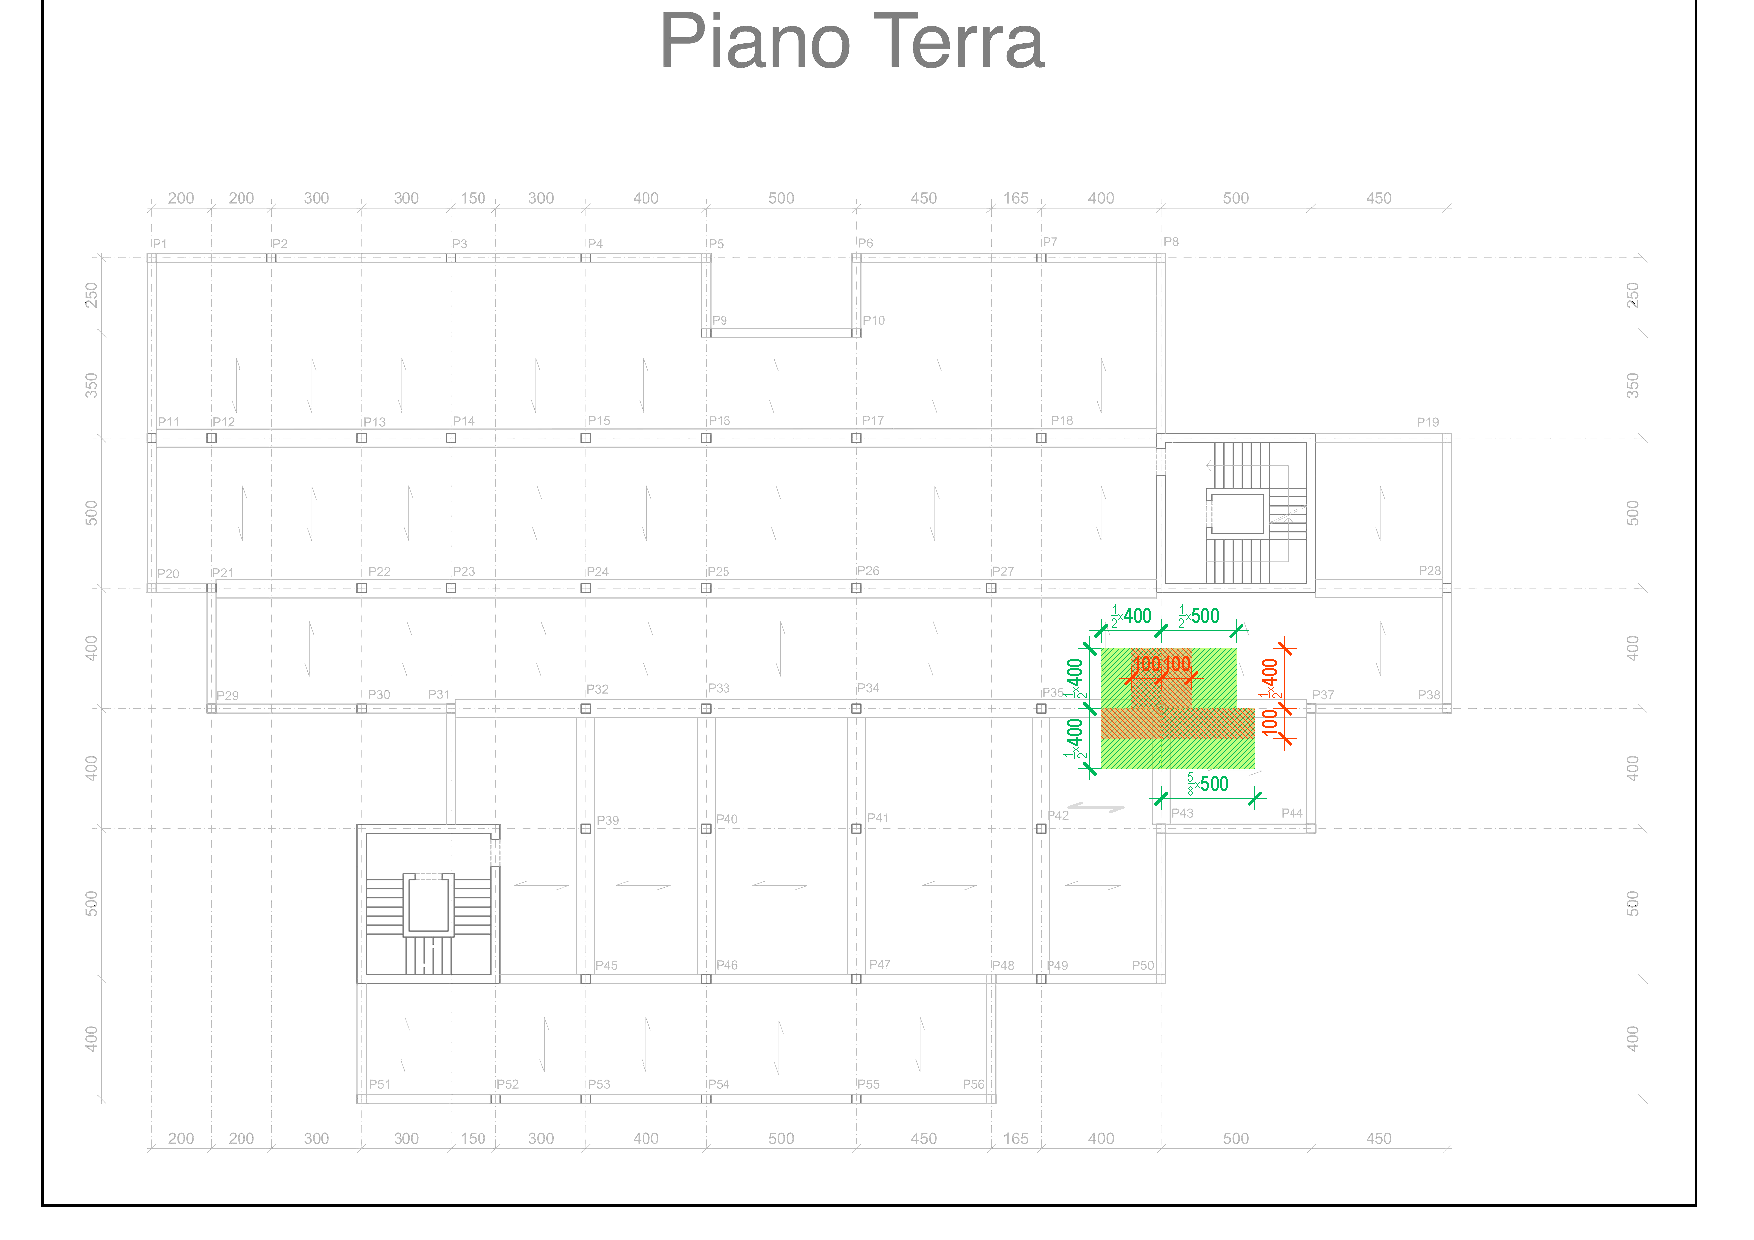
\includegraphics[trim=17.5cm 6.5cm 7cm 9.7cm,clip,frame]{IMG/Piante/Piante-PT.pdf}} \quad
\subfloat[][\emph{Piano Primo}]{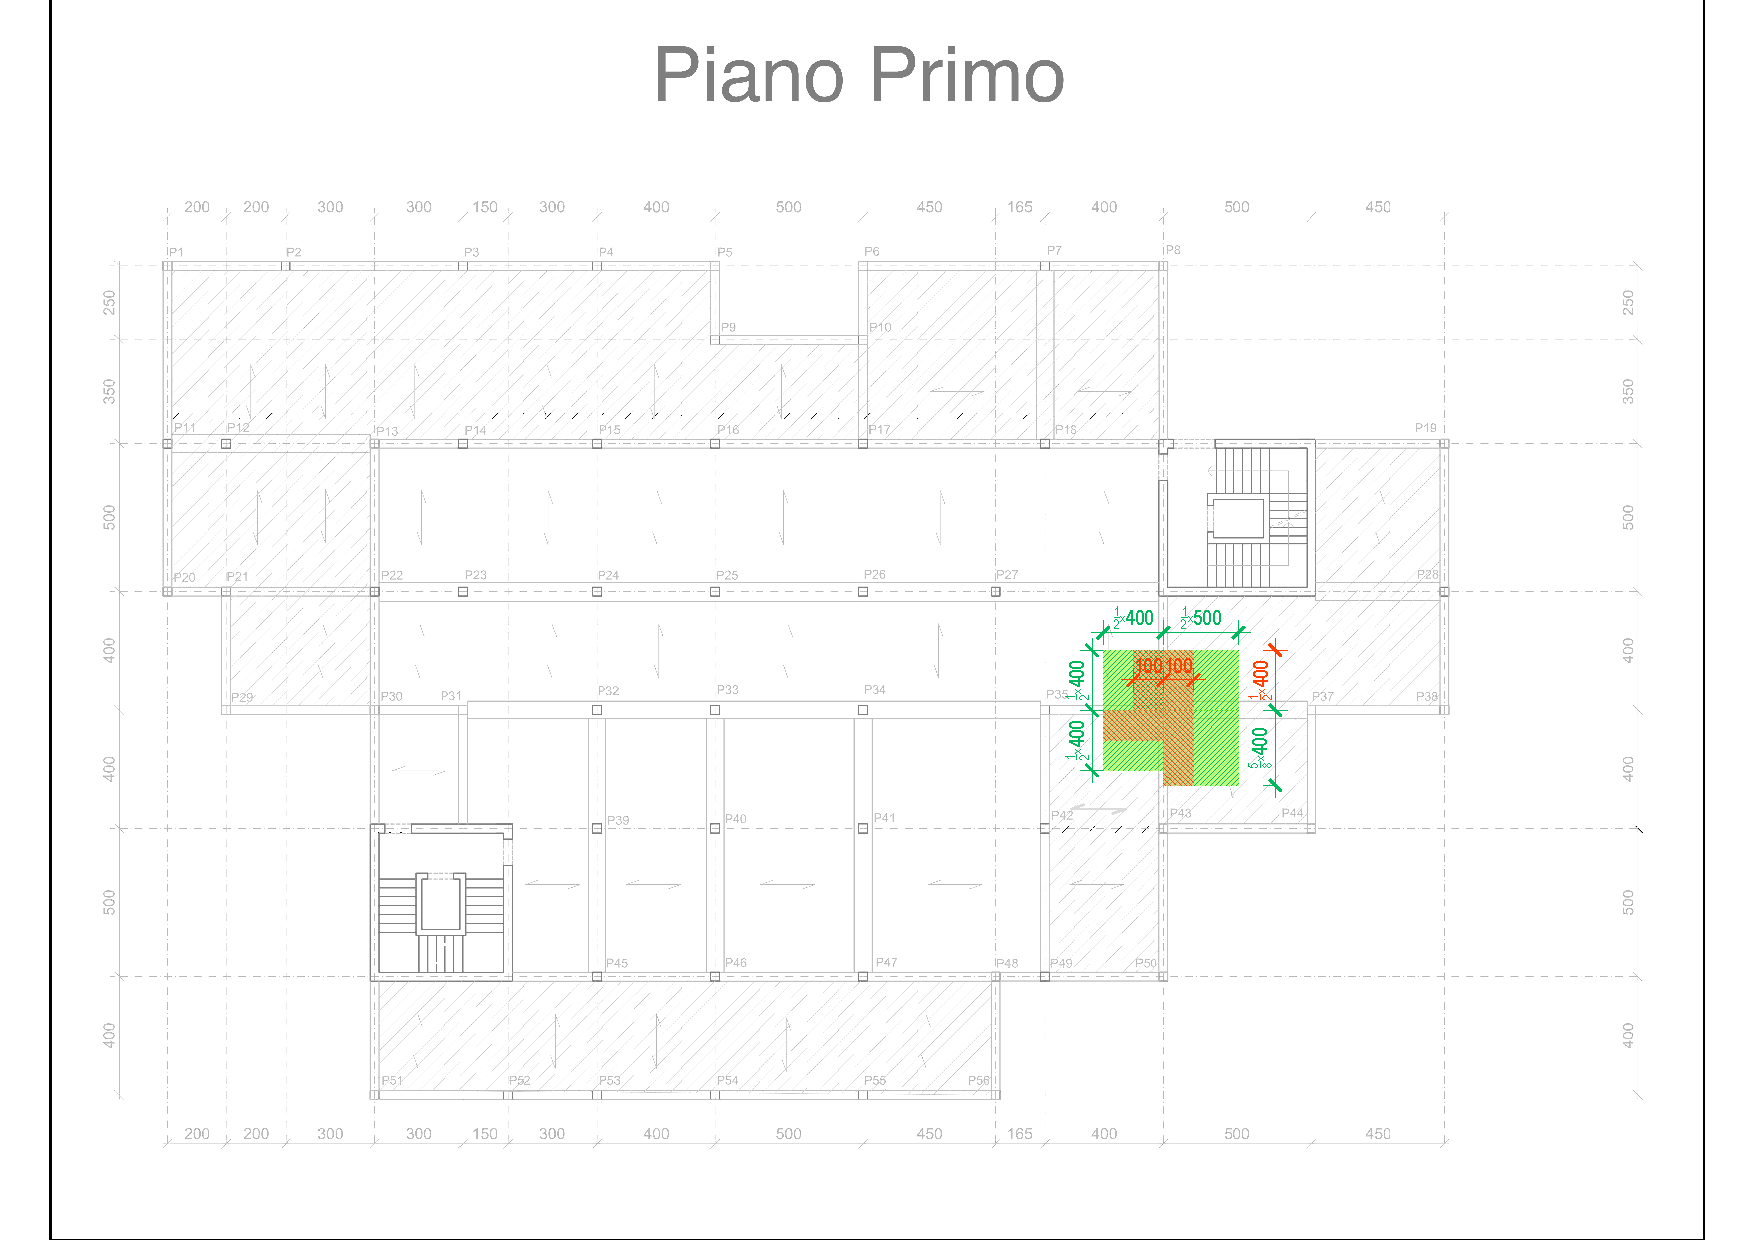
\includegraphics[trim=17.5cm 6.5cm 7cm 9.7cm,clip,frame]{IMG/Piante/Piante-P1.pdf}} \\
\subfloat[][\emph{Piano Secondo}]{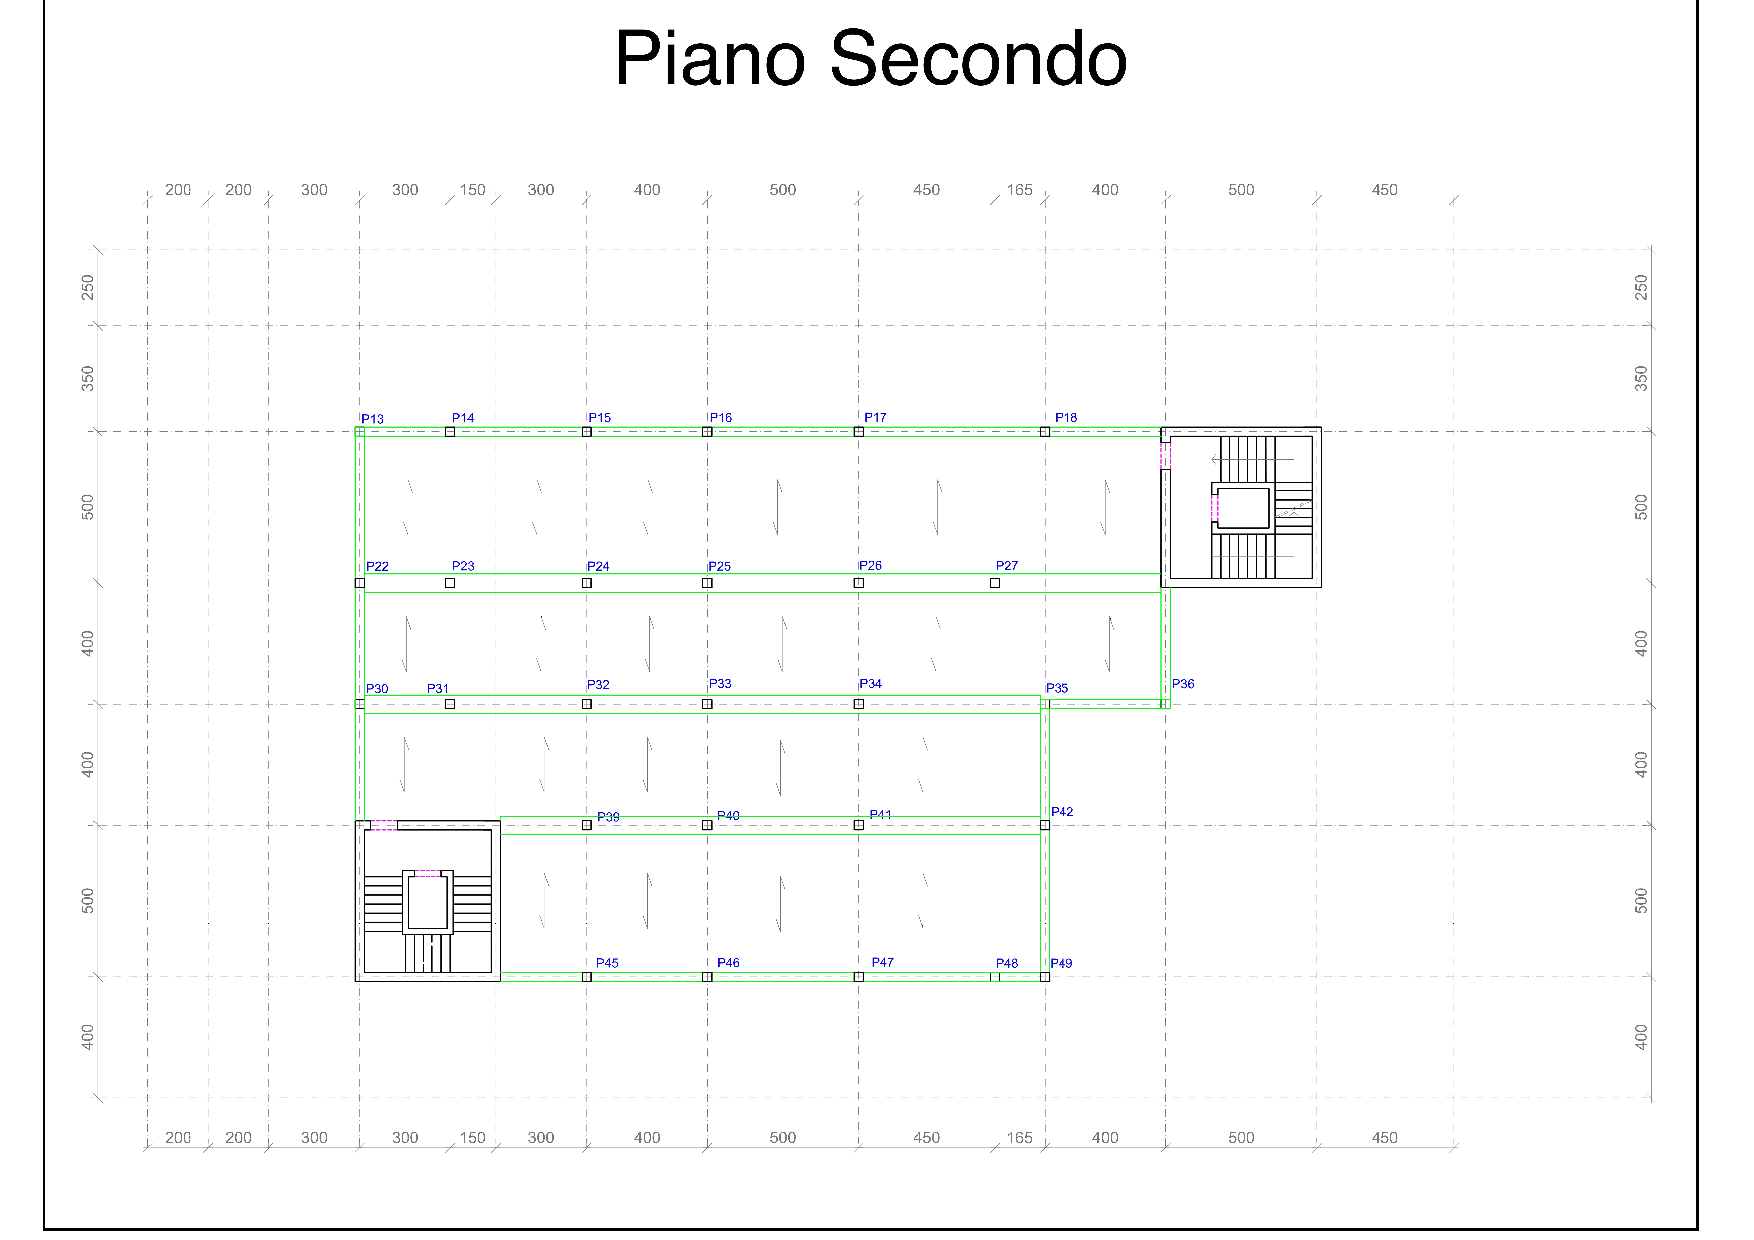
\includegraphics[trim=17.5cm 6.5cm 7cm 9.7cm,clip,frame]{IMG/Piante/Piante-P2.pdf}} \quad
\subfloat[][\emph{Piano Copertura}]{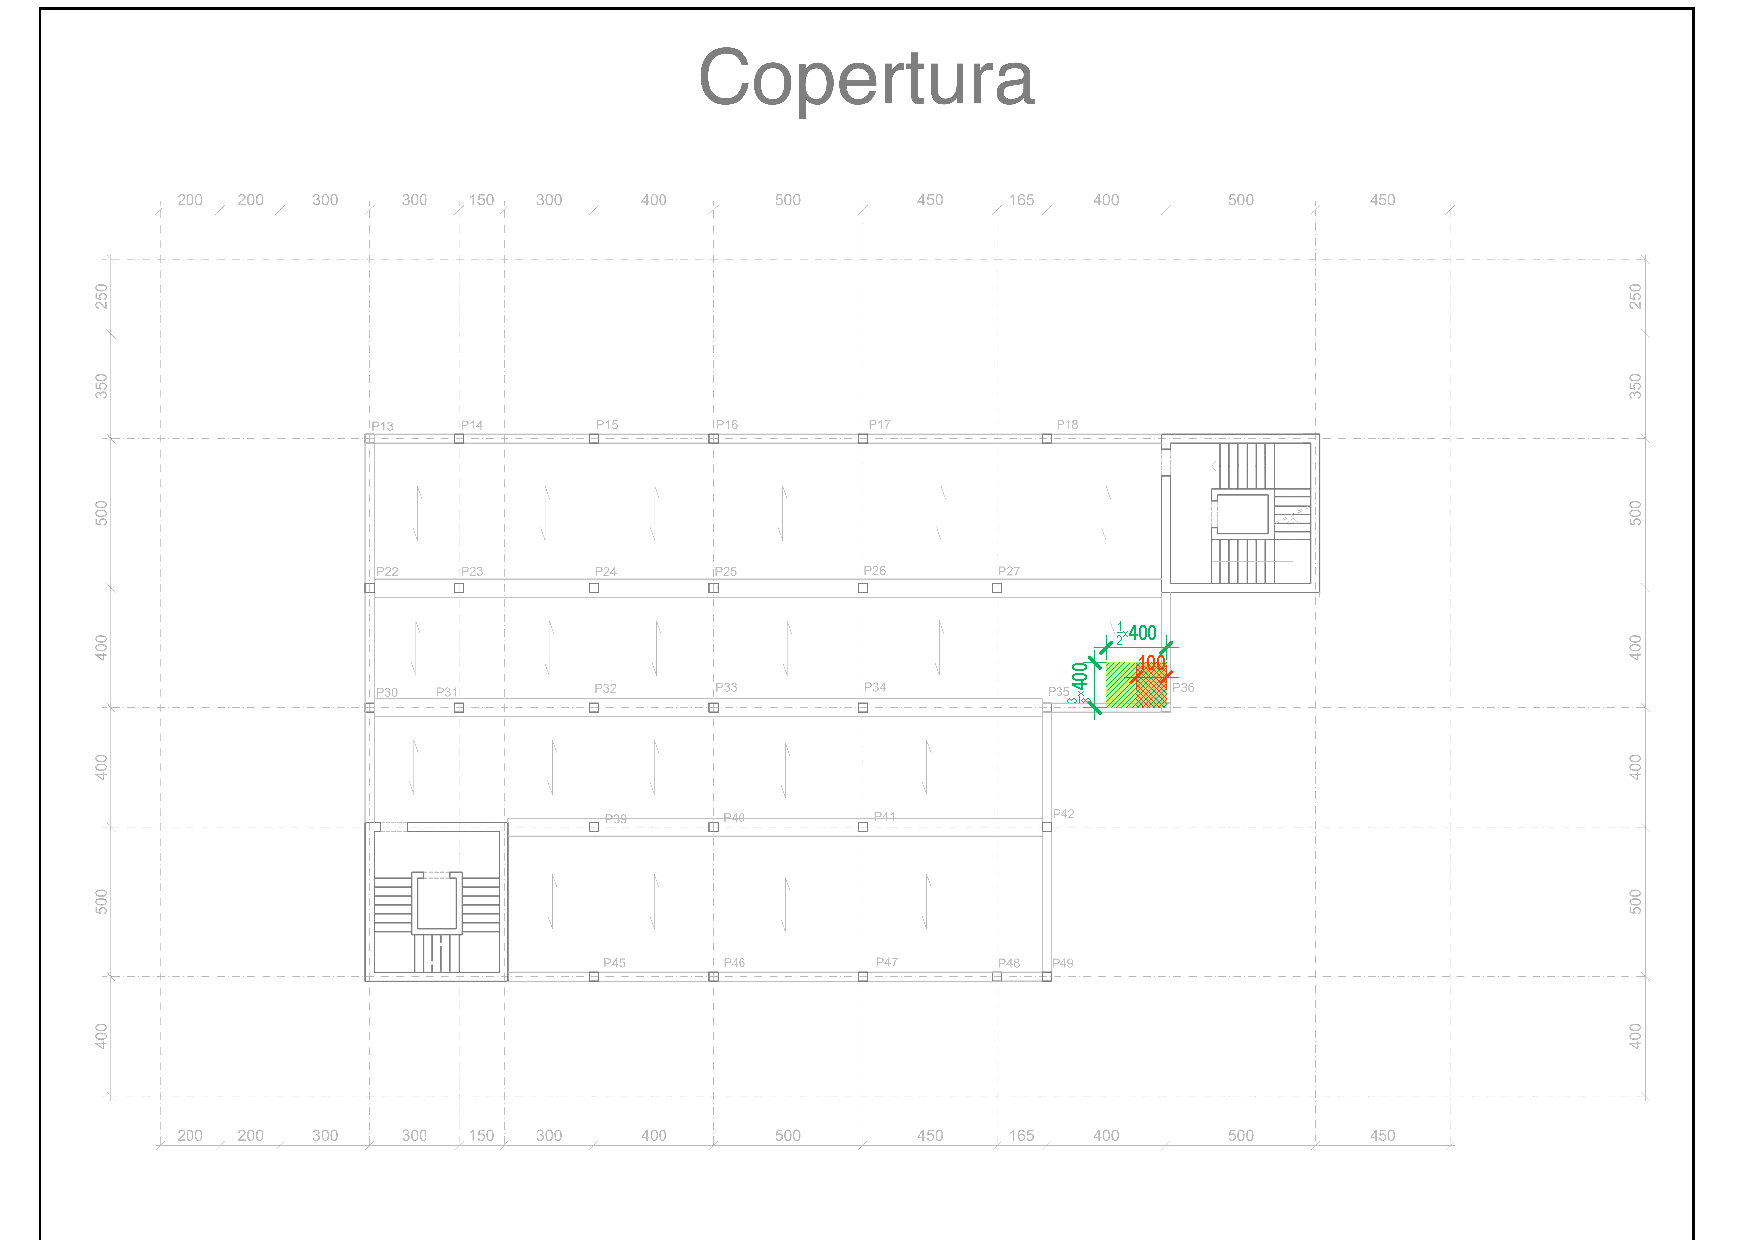
\includegraphics[trim=17.5cm 6.5cm 7cm 9.7cm,clip,frame]{IMG/Piante/Piante-PC.pdf}} \\
\caption{Indicazione delle aree di influenza gravanti sul pilastro P27}
\label{fig:AreeInfluenzaP27}
\end{figure}
In figura \ref{fig:AreeInfluenzaP27} vengono riportate schematicamente le aree di influenza agenti sul pilastro suddivise per ogni piano e con le relative quote. 
Si è considerato una lunghezza dimezzata nel caso la trave gravante sul pilastro fosse una trave interna, mentre una ripartizione di $3/8$ e $5/8$ nel caso di trave perimetrale. 
Si è considerato inoltre una striscia di influenza pari a \SI{1}{\meter} quando il solaio non fosse direttamente agente sulla trave ma parallelo ad essa. 
Sebbene ci siano delle aree sovrapposte si è voluto mantenerle a favore di sicurezza.
%!TEX root = ../RelazioneStrutturaleMeoliNicola.tex
\begin{figure}[htbp]
\centering
\begin{tikzpicture}
\draw[fill=black!20,thick] (0,0) rectangle node{\Huge$3$} (4,2);
\draw[fill=black!20,thick] (4,0) rectangle node{\Huge$4$} (8,2);
\draw[fill=black!20,thick] (0,2) rectangle node{\Huge$1$} (4,4);
\draw[fill=black!20,thick] (4,2) rectangle node{\Huge$2$} (8,4);
\draw[fill=black!30,ultra thick,opacity=0.4] (3.5,1.5) rectangle (4.5,2.5);
\end{tikzpicture}
\caption{Nomenclatura delle quattro aree che circondano il pilastro. Viene utilizzata nelle tabelle in cui vi è riportata l'estensione delle stesse e il relativo calcolo dello sforzo assiale.}
\label{fig:NomenclaturaAree}
\end{figure}
Si riporta infine in figura \ref{fig:NomenclaturaAree} la nomenclatura utilizzata per distinguere le quattro diverse aree e che viene utilizzata nei calcoli presenti nelle tabelle del paragrafo successivo.
\section{Totale carichi agenti sul pilastro}
Nelle tabelle sottostanti si riportano i carichi assiali ottenuti moltiplicando le estensioni delle aree i-esime per i relativi carichi di superficie appena trovati che sono agenti su di esse, sommati poi al peso proprio del pilastro relativo a quel piano ed eventualmente alle pareti perimetrali se presenti.
I valori di carico infine riportati sono quelli che verranno usati nel paragrafo successivo per la determinazione delle combinazioni di carico.
\paragraph*{Piano interrato} $G_1^{PI}=G_1^{pil.}=\SI{6.188}{\kilo\newton}$
\paragraph*{Piano terra} 
\begin{center}
\begin{tabular}{cS[table-format=1.2]S[table-format=3.2]S[table-format=3.2]S[table-format=3.2]}
	\toprule
	\multirow{2}{*}{Area n.}&\multicolumn{1}{c}{Estensione} & \multicolumn{1}{c}{$G_{1,k}^{PT}$}&\multicolumn{1}{c}{$G_{2,k}^{PT}$}&\multicolumn{1}{c}{$Q_{cat. D1,k}^{PT}$}\\
    &\multicolumn{1}{c}{$\left[\SI{}{\square\meter}\right]$} &\multicolumn{1}{c}{$\left[\SI{}{\kilo\newton}\right]$}&\multicolumn{1}{c}{$\left[\SI{}{\kilo\newton}\right]$}&\multicolumn{1}{c}{$\left[\SI{}{\kilo\newton}\right]$} \\
    \midrule
		$1$ & 5.63 & 20.25 & 28.24 & 22.50 \\
		$2$ & 7.06 & 25.43 & 35.45 & 28.25 \\
		$3$ & 4.50 & 16.20 & 22.59 & 18.00 \\
		$4$ & 5.65 & 20.34 & 28.36 & 22.60 \\
	\midrule
	\multicolumn{2}{l}{Totale =}	& 82.22 & 114.6 & 91.35\\	
	\bottomrule
\end{tabular}
\end{center}
Sommando il peso proprio del pilastro relativo al piano terra considerando l'altezza di interpiano di \SI{3.50}{\meter} si ha 
\begin{align*}
G_1^{PT} &= G_1^{pil.} + G_1^{sol.} = \SI{7.875}{} + \SI{82.22}{} =\SI{90.09}{\kilo\newton}\\
G_2^{PT} &= \SI{114.6}{\kilo\newton}\\
Q_{cat. D1}^{PT} &= \SI{91.35}{\kilo\newton}
\end{align*}
\paragraph*{Piano primo}
\begin{center}
\begin{tabular}{cS[table-format=1.2]S[table-format=3.2]S[table-format=3.2]S[table-format=3.2]}
	\toprule
	\multirow{2}{*}{Area n.}&\multicolumn{1}{c}{Estensione} & \multicolumn{1}{c}{$G_{1,k}^{P1}$}&\multicolumn{1}{c}{$G_{2,k}^{P1}$}&\multicolumn{1}{c}{$Q_{cat. B,k}^{P1}$}\\
    &\multicolumn{1}{c}{$\left[\SI{}{\square\meter}\right]$} &\multicolumn{1}{c}{$\left[\SI{}{\kilo\newton}\right]$}&\multicolumn{1}{c}{$\left[\SI{}{\kilo\newton}\right]$}&\multicolumn{1}{c}{$\left[\SI{}{\kilo\newton}\right]$} \\
    \midrule
		$1$ & 5.63 & 18.00 & 25.99 & 16.88 \\
		$2$ & 7.06 & 22.60 & 32.63 & 21.19 \\
		$3$ & 4.50 & 14.40 & 20.79 & 13.50 \\
		$4$ & 5.65 & 18.08 & 26.10 & 16.95 \\
	\midrule
	\multicolumn{2}{l}{Totale =}	& 73.08 & 105.5 & 68.51\\	
	\bottomrule
\end{tabular}
\end{center}
Sommando il peso proprio del pilastro relativo al piano terra con un'altezza di interpiano di \SI{3.10}{\meter} si ha 
\begin{align*}
G_1^{P1} &= G_1^{pil.} + G_1^{sol.} = \SI{6.975}{} + \SI{73.08}{} =\SI{80.06}{\kilo\newton}\\
G_2^{P1} &= \SI{105.51}{\kilo\newton}\\
Q_{cat. H}^{P1} &= \SI{68.51}{\kilo\newton}
\end{align*}
\paragraph*{Piano secondo}
\begin{center}
\begin{tabular}{cS[table-format=1.2]S[table-format=3.2]S[table-format=3.2]S[table-format=3.2]}
	\toprule
	\multirow{2}{*}{Area n.}&\multicolumn{1}{c}{Estensione} & \multicolumn{1}{c}{$G_{1,k}^{P2}$}&\multicolumn{1}{c}{$G_{2,k}^{P2}$}&\multicolumn{1}{c}{$Q_{cat. A,k}^{P2}$}\\
    &\multicolumn{1}{c}{$\left[\SI{}{\square\meter}\right]$} &\multicolumn{1}{c}{$\left[\SI{}{\kilo\newton}\right]$}&\multicolumn{1}{c}{$\left[\SI{}{\kilo\newton}\right]$}&\multicolumn{1}{c}{$\left[\SI{}{\kilo\newton}\right]$} \\
    \midrule
		$1$ & 5.63 & 18.00 & 25.99 & 11.25 \\
		$2$ & 7.06 & 22.60 & 32.63 & 14.13 \\
		$3$ & 4.50 & 14.40 & 20.79 & 9.000  \\
		$4$ & 7.06 & 22.60 & 32.63 & 14.13 \\
	\midrule
	\multicolumn{2}{l}{Totale =}	& 77.60 & 112.0 & 48.50\\	
	\bottomrule
\end{tabular}
\end{center}
Sommando il peso proprio del pilastro relativo al piano terra si ha 
\begin{align*}
G_1^{P2} &= G_1^{pil.} + G_1^{sol.} = \SI{6.975}{} + \SI{77.60}{} =\SI{84.58}{\kilo\newton}\\
G_2^{P2} &= \SI{112.0}{\kilo\newton}\\
Q_{cat. A}^{P2} &= \SI{48.50}{\kilo\newton}
\end{align*}
\paragraph*{Copertura}
\begin{center}
\begin{tabular}{cS[table-format=1.2]S[table-format=3.2]S[table-format=3.2]S[table-format=1.3]S[table-format=1.3]S[table-format=1.3]}
	\toprule
	\multirow{2}{*}{Area n.}&\multicolumn{1}{c}{Estensione} & \multicolumn{1}{c}{$G_{1,k}^{PC}$}&\multicolumn{1}{c}{$G_{2,k}^{PC}$}&\multicolumn{1}{c}{$Q_{cat. H,k}^{PC}$}&\multicolumn{1}{c}{$Q_{neve,k}^{PC}$}&\multicolumn{1}{c}{$Q_{vento,k}^{PC}$}\\
    &\multicolumn{1}{c}{$\left[\SI{}{\square\meter}\right]$} &\multicolumn{1}{c}{$\left[\SI{}{\kilo\newton}\right]$}&\multicolumn{1}{c}{$\left[\SI{}{\kilo\newton}\right]$}&\multicolumn{1}{c}{$\left[\SI{}{\kilo\newton}\right]$}&\multicolumn{1}{c}{$\left[\SI{}{\kilo\newton}\right]$}&\multicolumn{1}{c}{$\left[\SI{}{\kilo\newton}\right]$} \\
    \midrule
		$1$ & 5.63 & 20.25 & 15.98 & 2.813 & 7.318 & 0.649 \\
		$2$ & 7.06 & 25.43 & 20.06 & 3.531 & 9.188 & 0.815 \\
		$3$ & 4.50 & 16.20 & 12.78 & 2.250 & 5.855 & 0.519  \\
		$4$ & 7.06 & 25.43 & 20.06 & 3.531 & 9.188 & 0.815 \\
	\midrule
	\multicolumn{2}{l}{Totale =}	& 87.30 & 68.87 & 12.13 & 31.55 & 2.798\\	
	\bottomrule
\end{tabular}
\end{center}
In questo caso non c'è il contributo del peso proprio del pilastro, per cui i valori sono direttamente quelli riportati nel totale della tabella.
\section{Combinazioni di carico}
Per combinare i carichi si è assunta l'ipotesi di sovrapposizione delle forze. 
Ovvero si trova la combinazione peggiore per ciascun piano e si sommano per ottenere quella totale.
A differenza della trave non ci sono casi favorevoli o sfavorevoli ma agiranno soltanto questi ultimi.

Si elencano ora tutte le possibili combinazioni per ciascun piano, infine nel paragrafo successivo si riportano in TABELLA DA METTERE quelli con valore più grande e la somma di essi.
Si riporta poi in FIGURA DA METTERE una rappresentazione dell'andamento del carico assiale sul pilastro in questione.
\paragraph*{Piano interrato} Il contributo corrispondente al solo pilastro tra solaio piano interrato e solaio piano terra è
\begin{align*}
SLU^{\text{sfav}}&= \gamma_{G1}\cdot G_1 = 1.3\cdot\SI{8.044}{} =\SI{426.0}{\kilo\newton}\\
SLE &= \gamma_{G1}\cdot G_1 = \cdot\SI{6.188}{} =\SI{6.188}{\kilo\newton}
\end{align*}
\paragraph*{Piano Terra} Essendoci un solo carico variabile si ha una sola combinazione per tipologia di stato:
\begin{align} 
	\begin{split}
	SLU^{\text{sfav}}_{\text{cat. D1}} &= \gamma_{G1}\cdot G_1 + \gamma_{G2} \cdot G_2 + \gamma_{cat. D1} \cdot Q_{cat. D1}\\
	&= 1.3\cdot\SI{90.09}{} + 1.5\cdot\SI{114.6}{} + 1.5\cdot\SI{91.35}{} \\
	&= \SI{426.0}{\kilo\newton}
	\end{split} \\  
	\begin{split}
	SLE^{\text{rara}}_{\text{cat. D1}} &= G_1 + G_2 + Q_{cat. D1}\\
	&= \SI{90.09}{} + \SI{114.6}{} + \SI{91.35}{}\\
	&= \SI{296.0}{\kilo\newton}
	\end{split} \\ 
	\begin{split}
	SLE^{\text{frequente}}_{\text{cat. D1}} &= G_1 + G_2 + \psi_{11}\cdot Q_{cat. D1}\\
	&= \SI{90.09}{} + \SI{114.6}{} + 0.7\cdot\SI{91.35}{}\\
	&= \SI{268.6}{\kilo\newton}
	\end{split} \\ 
	\begin{split}
	SLE^{\text{quasi perm.}}_{\text{cat. D1}} &= G_1 + G_2 + \psi_{21}\cdot Q_{cat. D1}\\
	&= \SI{90.09}{} + \SI{114.6}{} + 0.6\cdot\SI{91.35}{}\\
	&= \SI{259.5}{\kilo\newton}
	\end{split} 
\end{align}
Analogamente si ha
\paragraph*{Piano primo}
\begin{align*} 
	SLU^{\text{sfav}}_{\text{cat. B}}		&= \SI{365.1}{\kilo\newton} \\	
	SLE^{\text{rara}}_{\text{cat. B}} 		&= \SI{254.1}{\kilo\newton} \\
	SLE^{\text{frequente}}_{\text{cat. B}} 	&= \SI{219.8}{\kilo\newton} \\
	SLE^{\text{quasi perm.}}_{\text{cat. B}}&= \SI{206.1}{\kilo\newton}
\end{align*}
\paragraph*{Piano secondo}
\begin{align*} 
	SLU^{\text{sfav}}_{\text{cat. A}}		&= \SI{350.7}{\kilo\newton} \\	
	SLE^{\text{rara}}_{\text{cat. A}} 		&= \SI{245.1}{\kilo\newton} \\
	SLE^{\text{frequente}}_{\text{cat. A}} 	&= \SI{220.8}{\kilo\newton} \\
	SLE^{\text{quasi perm.}}_{\text{cat. A}}&= \SI{211.1}{\kilo\newton}
\end{align*}
\paragraph*{Copertura} Per la copertura invece si sono considerati tutti e tre i carichi variali 
\begin{align} 
	\begin{split}
	SLU^{\text{sfav}}_{\text{cat. H}} &= \gamma_{G1}\cdot G_1 + \gamma_{G2} \cdot G_2 + \gamma_{cat. H} \cdot Q_{cat. H} + \gamma_{neve}\cdot Q_{neve}\cdot\psi_{02} + \gamma_{vento}\cdot Q_{vento} \cdot \psi_{03}  \\
	&= 1.3\cdot\SI{87.30}{} + 1.5\cdot\SI{68.87}{} + 1.5\cdot\SI{12.13}{} + 1.5\cdot\SI{31.55}{}\cdot0.5 + 1.5\cdot\SI{2.798}{}\cdot0.6\\
	&= \SI{261.2}{\kilo\newton}
	\end{split} \\ 
	\begin{split}
	SLU^{\text{sfav}}_{\text{neve}} &= \gamma_{G1}\cdot G_1 + \gamma_{G2} \cdot G_2 + \gamma_{neve}\cdot Q_{neve} + \gamma_{cat. H} \cdot Q_{cat. H}\cdot\psi_{02} + \gamma_{vento}\cdot Q_{vento} \cdot \psi_{03}  \\
	&= 1.3\cdot\SI{87.30}{} + 1.5\cdot\SI{68.87}{} + 1.5\cdot\SI{31.55}{} + \varnothing + 1.5\cdot\SI{2.798}{}\cdot0.6\\
	&= \SI{266.6}{\kilo\newton}
	\end{split} \\ 
	\begin{split}
	SLU^{\text{sfav}}_{\text{vento}} &= \gamma_{G1}\cdot G_1 + \gamma_{G2} \cdot G_2 + \gamma_{vento}\cdot Q_{vento} + \gamma_{cat. H} \cdot Q_{cat. H}\cdot\psi_{02} + \gamma_{neve}\cdot Q_{neve} \cdot \psi_{03}  \\
	&= 1.3\cdot\SI{87.30}{} + 1.5\cdot\SI{68.87}{} + 1.5\cdot\SI{2.798}{} + \varnothing + 1.5\cdot\SI{31.55}{}\cdot0.5\\
	&= \SI{244.7}{\kilo\newton}
	\end{split} \\ 
	\begin{split}
	SLE^{\text{rara}}_{\text{cat. H}} &= G_1 + G_2 + Q_{cat. H} + \psi_{02}\cdot Q_{neve} + \psi_{03}\cdot Q_{vento}  \\
	&= \SI{87.30}{} + \SI{68.87}{} + \SI{12.13}{} + 0.5\cdot\SI{31.55}{} + 0.6\cdot\SI{2.798}{}\\
	&= \SI{185.7}{\kilo\newton}
	\end{split} \\ 
	\begin{split}
	SLE^{\text{rara}}_{\text{neve}} &= G_1 + G_2 + Q_{neve} + \psi_{02}\cdot Q_{cat. H} + \psi_{03}\cdot Q_{vento}  \\
	&= \SI{87.30}{} + \SI{68.87}{} + \SI{31.55}{} + \varnothing + 0.6\cdot\SI{2.798}{}\\
	&= \SI{189.4}{\kilo\newton}
	\end{split} \\ 
	\begin{split}
	SLE^{\text{rara}}_{\text{vento}} &= G_1 + G_2 + Q_{vento} + \psi_{02}\cdot Q_{cat. H} + \psi_{03}\cdot Q_{neve}  \\
	&= \SI{87.30}{} + \SI{68.87}{} + \SI{2.798}{} + \varnothing + 0.6\cdot\SI{31.55}{}\\
	&= \SI{174.7}{\kilo\newton}
	\end{split} \\ 
	\begin{split}
	SLE^{\text{frequente}}_{\text{cat. H}} &= G_1 + G_2 + \psi_{11}\cdot Q_{cat. H} + \psi_{22}\cdot Q_{neve} + \psi_{23}\cdot Q_{vento}  \\
	&= \SI{87.30}{} + \SI{68.87}{} + 0.5\cdot\SI{12.13}{} + \varnothing +\varnothing\\
	&= \SI{156.2}{\kilo\newton}
	\end{split} \\ 
	\begin{split}
	SLE^{\text{frequente}}_{\text{neve}} &= G_1 + G_2 + \psi_{11}\cdot Q_{neve} + \psi_{22}\cdot Q_{cat. H} + \psi_{23}\cdot Q_{vento}  \\
	&= \SI{87.30}{} + \SI{68.87}{} + 0.2\cdot\SI{31.55}{} + \varnothing + \varnothing \\
	&= \SI{162.5}{\kilo\newton}
	\end{split} \\ 
	\begin{split}
	SLE^{\text{frequente}}_{\text{vento}} &= G_1 + G_2 + \psi_{11}\cdot Q_{vento} + \psi_{22}\cdot Q_{cat. H} + \psi_{23}\cdot Q_{neve}  \\
	&= \SI{87.30}{} + \SI{68.87}{} + 0.2\cdot\SI{2.798}{} + \varnothing + \varnothing\\
	&= \SI{156.7}{\kilo\newton}
	\end{split} \\ 
	\begin{split}
	SLE^{\text{quasi perm.}} &= G_1 + G_2 + \psi_{21}\cdot Q_{cat. H} + \psi_{22}\cdot Q_{neve} + \psi_{23}\cdot Q_{vento} \\
	&= \SI{87.30}{} + \SI{68.87}{} + \varnothing + \varnothing + \varnothing \\
	&= \SI{156.2}{\kilo\newton}
	\end{split} 
\end{align}

\section{Totale agente sul pilastro}
Prendendo il valore massimo tra le combinazioni e sommando si ottengono i massimi carichi assiali possibili sul pilastro P27.
\begin{align*} 
	SLU^{\text{sfav}}_{\text{P27}}		n&= \SI{1416}{\kilo\newton} \\	
	SLE^{\text{rara}}_{\text{P27}} 		 &= \SI{990.8}{\kilo\newton} \\
	SLE^{\text{frequente}}_{\text{P27}}  &= \SI{878.0}{\kilo\newton} \\
	SLE^{\text{quasi perm.}}_{\text{P27}}&= \SI{839.1}{\kilo\newton}
\end{align*}
\e possibile inoltre fare un grafico l'andamento dei carichi in funzione della quota dell'edificio.
Si ha infatti un valore costante nel passaggio tra un piano e l'altro e un andamento lineare crescente lungo l'altezza del pilastro dovuto al peso proprio crescente.

\begin{figure}[htb]
\centering
\begin{tikzpicture}
	\begin{axis}[
		/pgf/number format/.cd,
        use comma,      %virgola nei decimali
        1000 sep={\,},  %uno spazio nelle migliaia
	    height=12cm,
		width=\textwidth,
		grid=major,
		xlabel=Sforzo assiale cumulato \si{[\kilo\newton]},
		ylabel=Altezza edificio \si{[\meter]},
		ytick = {9.7,6.6,3.5,0,-2.75},
		%title=Titolo se serve
    ]
	\addplot[thick,color=red] coordinates {
	   (0000.00, 9.7  )
	   (0266.64, 9.7  )
	   (0275.70, 6.6  )
	   (0617.34, 6.6  )
	   (0626.41, 3.5  )
	   (0982.45, 3.5  )
	   (0992.69, 0    )
	   (1408.49, 0    )
	   (1416.53, -2.75)
	};
	\addplot[thick,color=blue] coordinates {
	   (0000.00,  9.7  )
	   (0189.40, 9.7  )
	   (0196.37, 6.6  )
	   (0434.48, 6.6  )
	   (0441.45, 3.5  )
	   (0680.68, 3.5  )
	   (0688.56, 0    )
	   (0978.41, 0    )
	   (0990.79, -2.75)
	};
	\addplot[thick,color=green] coordinates {
	   (0000.00,  9.7  )
	   (0162.48, 9.7  )
	   (0169.45, 6.6  )
	   (0390.28, 6.6  )
	   (0383.31, 3.5  )
	   (0595.26, 3.5  )
	   (0603.13, 0    )
	   (0865.58, 0    )
	   (0877.96, -2.75)
	};
	\addplot[thick,color=magenta] coordinates {
	   (0000.00,  9.7  )
	   (0156.17, 9.7  )
	   (0163.15, 6.6  )
	   (0367.30, 6.6  )
	   (0374.28, 3.5  )
	   (0565.55, 3.5  )
	   (0573.42, 0    )
	   (0826.74, 0    )
	   (0839.11, -2.75)
	};
	\legend{SLU,SLE Rara,SLE Frequente,SLE Quasi Permanente}
	\end{axis}
\end{tikzpicture}
\caption{Andamento dello sforzo assiale agente sul pilastro P27 in funzione dell'altezza}
%\label{fig:}
\end{figure}
%!TEX root = ../RelazioneStrutturaleMeoliNicola.tex
\chapter{Pilastro P36}
Valgono le stesse considerazioni affrontate per il pilastro P27.
La suddivisione dei piani è la stessa. 
In aggiunta al caso precedente, il pilastro P36 ha il primo piano suddiviso in zona interna e zona terrazzo. 
Pertanto nel paragrafo relativo alle area di influenza saranno considerati i due contributi distinti.
Verranno però poi considerati insieme nel calcolo delle combinazioni, in quanto essendo appartenenti alla stessa categoria si suppone che se il carico si massimizza in una zona, questo avverrà anche nell'altra.

Un'altra differenza nelle aree di influenza sta nel fatto che in certe parti, come si vede nelle figure che verranno riportate, sono presenti orditure parallele alla trave.
In queste zone si è preso come riferimento una lunghezza di riferimento di \SI{1}{\meter}. 

Infine al solaio del piano primo e del piano secondo sono presenti i contributi delle pareti perimetri.

Verranno ora analizzati solamente le differenze di carico rispetto al caso precedente. 
Infine verranno riportati i risultati finali e il grafico dell'andamento dello sforzo assiale.

\section{Analisi dei carichi}
\subsection{Piano Primo - Interno}
\paragraph*{G1 e G2}  Agiscono gli stessi solai visti nel capitolo riguardante la trave. 
\paragraph*{Categoria B} \e presente la categoria B.
Si utilizza quindi \SI{3.00}{\kilo\newton\per\square\meter}
\subsection{Piano Primo - Terrazzo} 
\paragraph*{G1 e G2} Agiscono gli stessi solai visti nel capitolo riguardante la trave. 
\paragraph*{G2 - Pareti perimetrali}
In questa zona agiscono in più anche le pareti perimetrali.
Esse hanno la medesima stratigrafia vista al paragrafo a pagina \pageref{cap:paretiPerimetrali} nella formula \eqref{eq:paretiPerimetrali}.
\paragraph*{Categoria B - balconi} \e presente la categoria B riferita ai balconi. 
Si utilizza quindi \SI{4.00}{\kilo\newton\per\square\meter}
\paragraph*{Neve} Si è adottato lo stesso procedimento visto per la trave in quanto anche qui è presente l'accumolo della neve.
In questo caso però è presente un angolo che causerebbe la somma dei due  contributi; perciò si è considerata un unico caso peggiore, ovvero quello con $b_2  = \SI{4.00}{\meter}.$
Il coefficiente di forma diviene pari a 
\begin{align*}
	\mu_w &= \frac{\SI{18.00}{}\cdot\SI{4.00}{}}{2\cdot\SI{6.20}{}}=1.774\\
    \begin{split}
		\mu_2 &=\mu_1 + \frac{(l_s - b_2)\cdot (\mu_w-\mu_1)}{l_s} \\
		      &= 0.8+\frac{(2\cdot\SI{6.20}{}-b_2)\cdot(1.774-0.8)}{2\cdot\SI{6.20}{}}\\
		      &= 1.460
    \end{split}\\
	\mu^{Ter.}&= \frac{\mu_w + \mu_2}{2}=1.617
\end{align*}
Gli altri coefficienti sono rimasti invariati, pertanto il carico della neve diviene
\[
	q_s^{P1} = q_{sk} \cdot C_E \cdot C_t \cdot \mu^{Ter.} = \SI{1.626}{} \cdot 1 \cdot 1 \cdot 1.617 = \SI{2.629}{\kilo\newton\per\square\meter}
\]
\paragraph*{Vento} Si utilizza lo stesso valore visto per il terrazzo nell'equazione \eqref{eq:caricoVento}.
\subsection{Riassumendo}
Si ha
\begin{center}
\begin{tabular}{lS[table-format=1.2]S[table-format=1.2]S[table-format=1.3]S[table-format=1.3]S[table-format=1.3]}
	\toprule
	\multirow{2}{*}{Piano}& \multicolumn{1}{c}{$g_{1,k}^{i}$}&\multicolumn{1}{c}{$g_{2,k}^{i}$}&\multicolumn{1}{c}{$q_{cat. j,k}^{i}$}&\multicolumn{1}{c}{$q_{neve,k}^{i}$}&\multicolumn{1}{c}{$Q_{vento,k}^{i}$}\\
    &\multicolumn{1}{c}{$\left[\SI{}{\kilo\newton\per\square\meter}\right]$}&\multicolumn{1}{c}{$\left[\SI{}{\kilo\newton\per\square\meter}\right]$}&\multicolumn{1}{c}{$\left[\SI{}{\kilo\newton\per\square\meter}\right]$}&\multicolumn{1}{c}{$\left[\SI{}{\kilo\newton\per\square\meter}\right]$}&\multicolumn{1}{c}{$\left[\SI{}{\kilo\newton\per\square\meter}\right]$} \\
    \midrule
		Terra                  & 3.60 & 5.02 & 4.00 &     &  \\
		Primo - Interno 	   & 3.20 & 4.62 & 3.00 &     & \\
		Primo - Terrazzo       & 3.20 & 2.215 & 4.00 &  2.629   & 0.1154  \\
		Secondo                & 3.20 & 4.62 & 2.00 &     &  \\
		Copertura              & 3.60 & 2.84 & 0.50 & 1.301    & 0.1154 \\
	\bottomrule
\end{tabular}
\end{center}
A cui vanno sommai i valori delle pareti perimetrali al piano Primo e Secondo.
\section{Aree di influenza}
\begin{figure}[htbp]
\centering
\subfloat[][\emph{Piano Terra}]{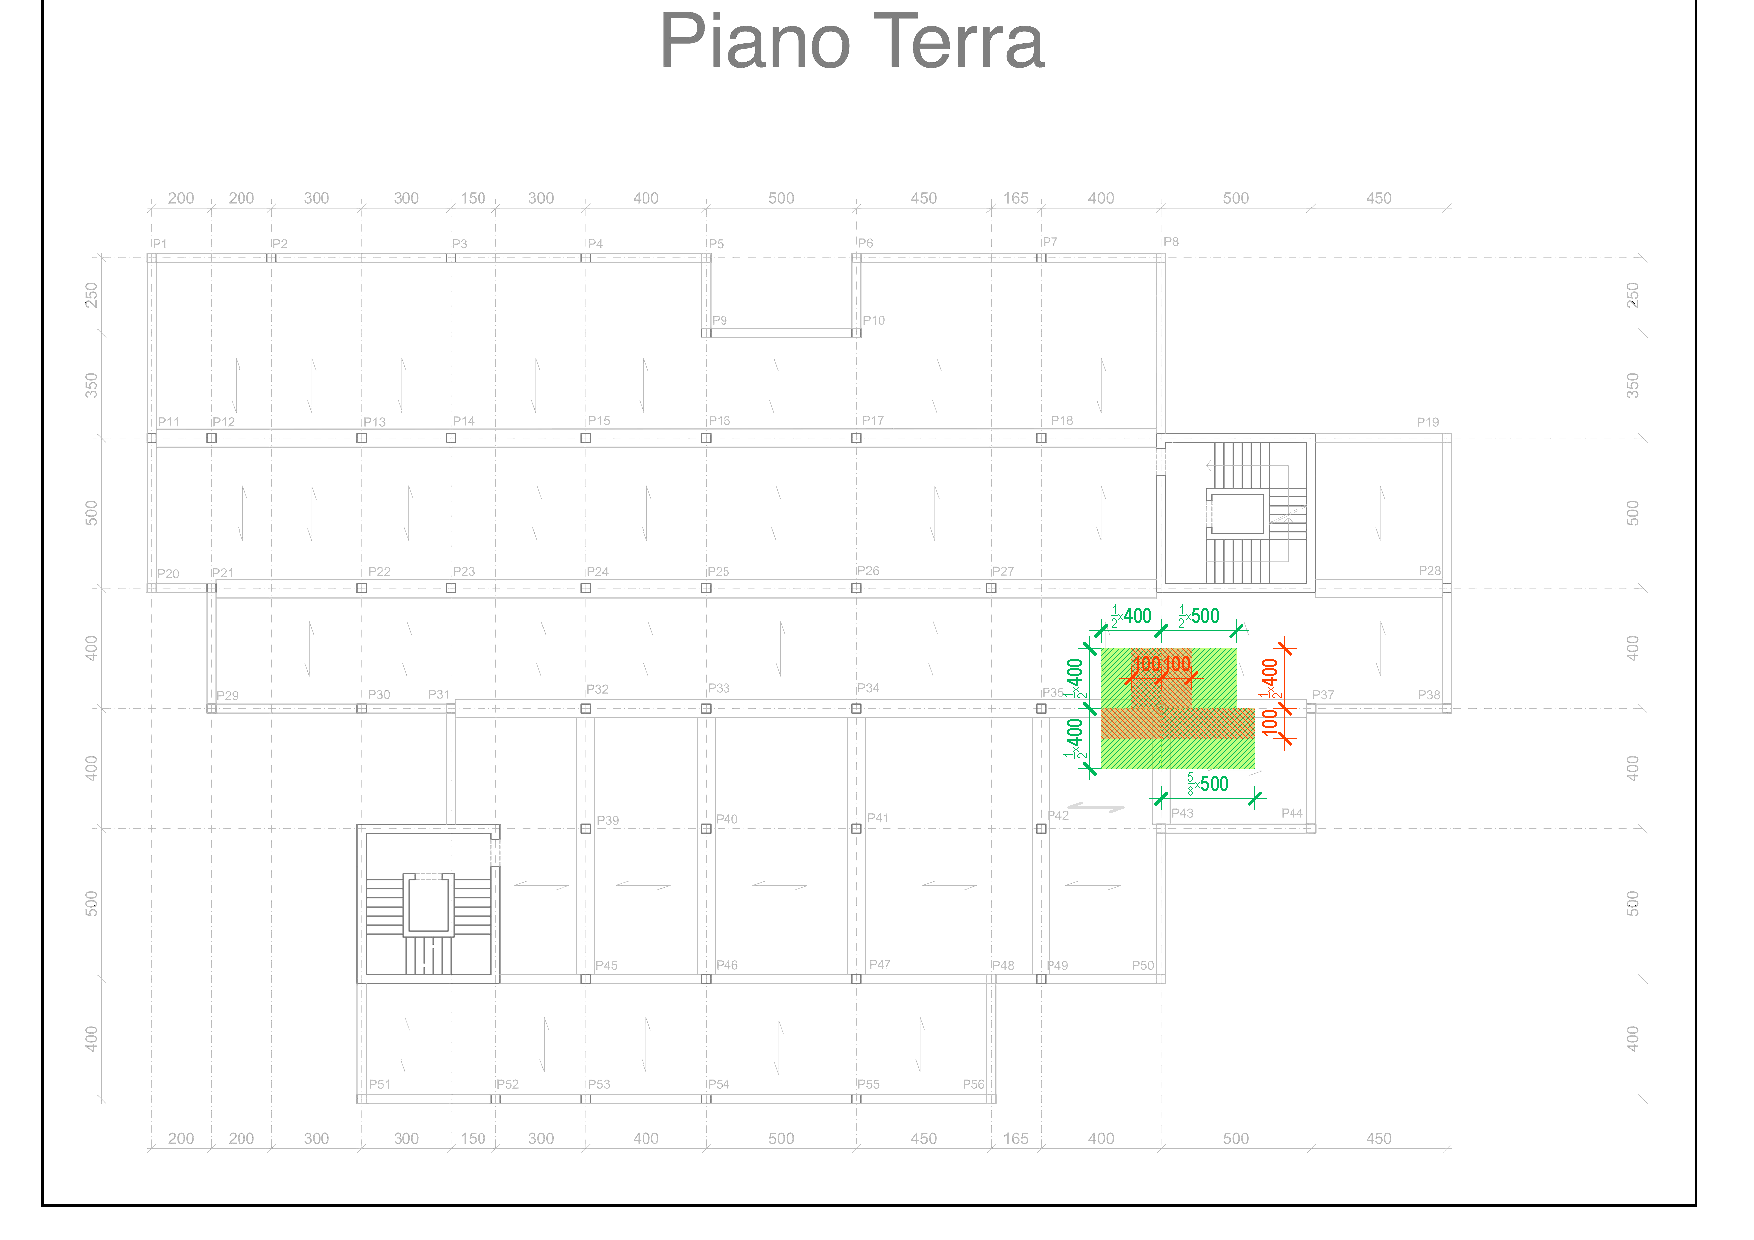
\includegraphics[trim=17.5cm 6.5cm 7cm 9.7cm,clip,frame]{IMG/Piante/Piante-PT.pdf}} \quad
\subfloat[][\emph{Piano Primo}]{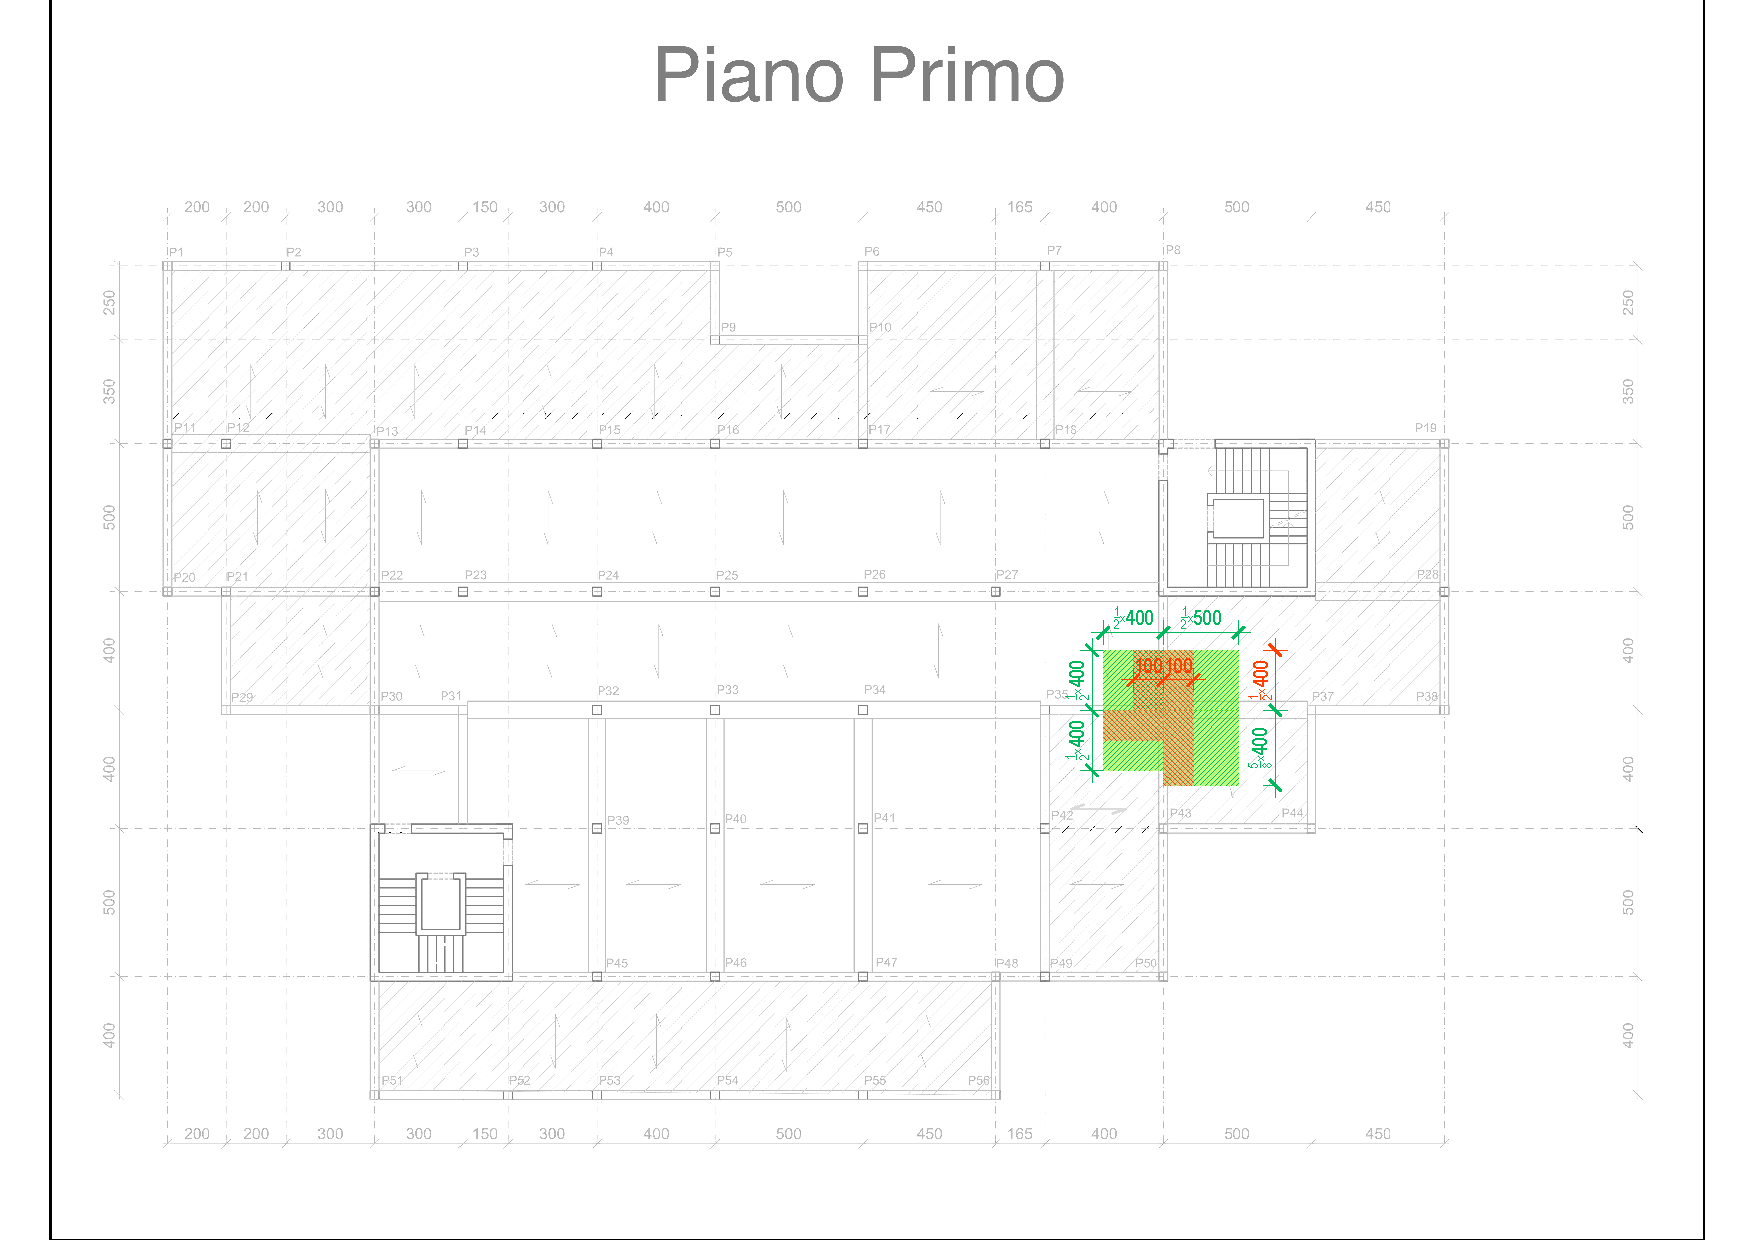
\includegraphics[trim=17.5cm 6.5cm 7cm 9.7cm,clip,frame]{IMG/Piante/Piante-P1.pdf}} \\
\subfloat[][\emph{Piano Secondo}]{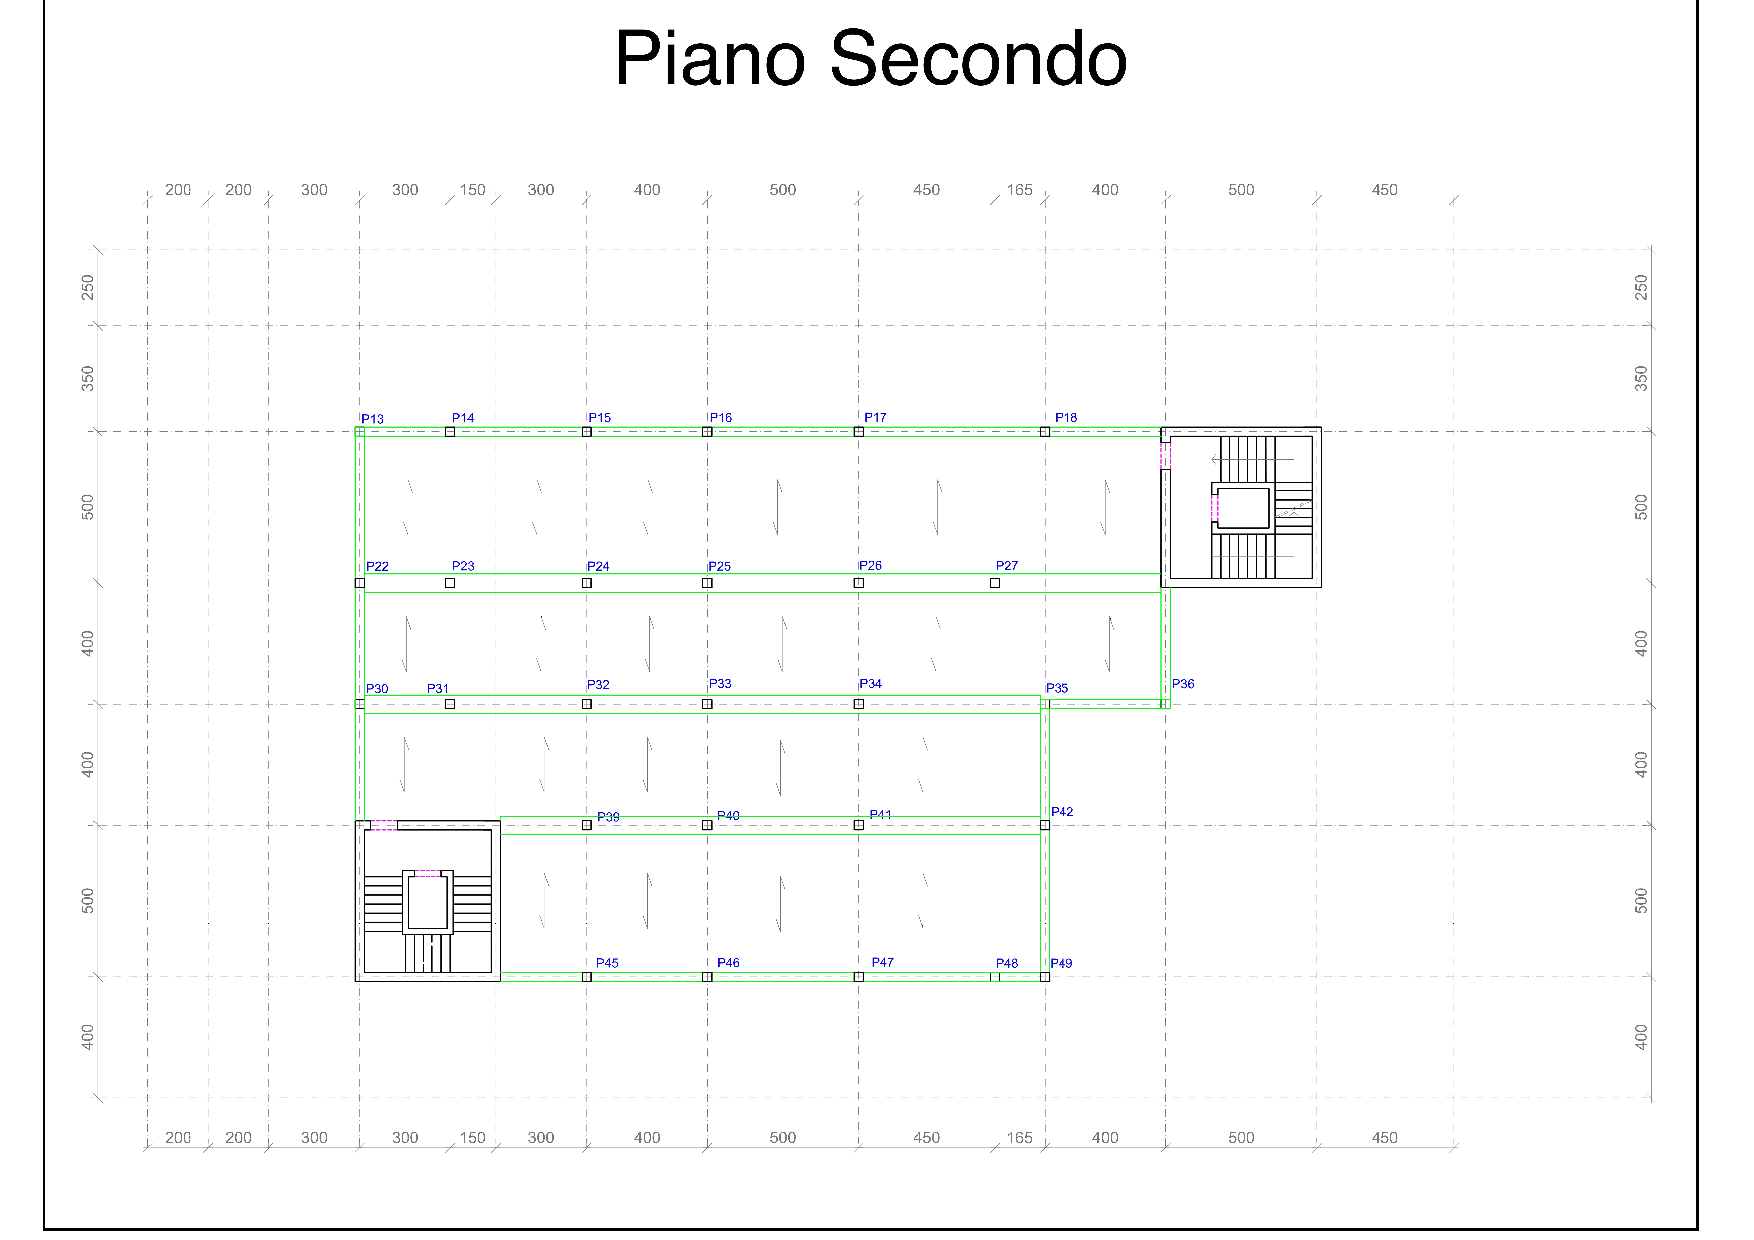
\includegraphics[trim=17.5cm 6.5cm 7cm 9.7cm,clip,frame]{IMG/Piante/Piante-P2.pdf}} \quad
\subfloat[][\emph{Piano Copertura}]{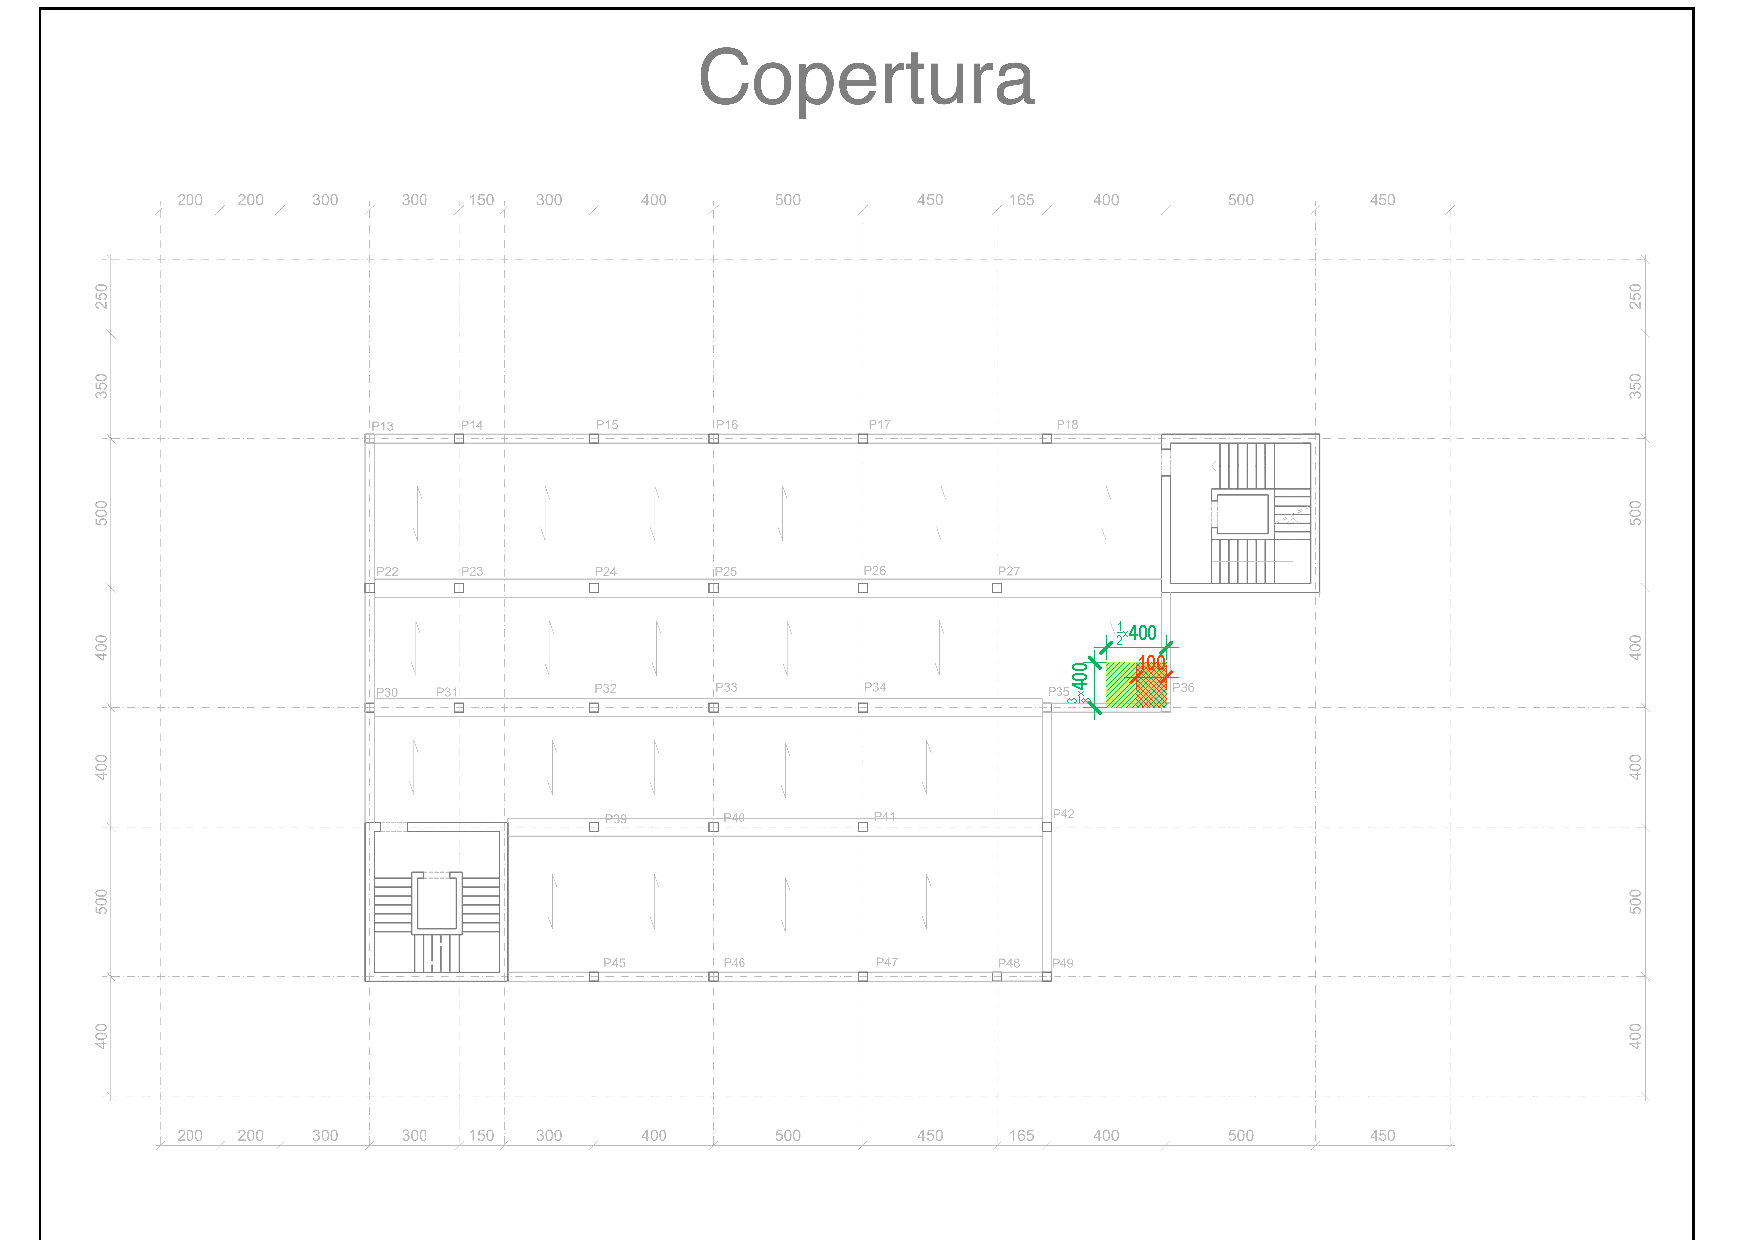
\includegraphics[trim=17.5cm 6.5cm 7cm 9.7cm,clip,frame]{IMG/Piante/Piante-PC.pdf}} \\
\caption{Indicazione delle aree di influenza gravanti sul pilastro P36}
\label{fig:AreeInfluenzaP36}
\end{figure}
In figura \ref{fig:AreeInfluenzaP36} vengono riportate schematicamente le aree di influenza agenti sul pilastro suddivise per ogni piano e con le relative quote. 
Si è considerato una lunghezza dimezzata nel caso la trave gravante sul pilastro fosse una trave interna, mentre una ripartizione di $3/8$ e $5/8$ nel caso di trave perimetrale. 
Si è considerato inoltre una striscia di influenza pari a \SI{1}{\meter} quando il solaio non fosse direttamente agente sulla trave ma parallelo ad essa. 
Sebbene ci siano delle aree sovrapposte si è voluto mantenerle a favore di sicurezza.
Vale la stessa nomenclatura utilizzata in precedenza mostrata in figura \ref{fig:NomenclaturaAree} a pagina \pageref{fig:NomenclaturaAree}.

In aggiunta alle aree è presente la quota parte delle pareti perimetrali che scaricano sul pilastro. 
Si è considerato metà della lunghezza del lato, per entrambi i lati.
\section{Totale carichi agenti sul pilastro}
Nelle tabelle sottostanti si riportano i carichi assiali ottenuti moltiplicando le estensioni delle aree i-esime per i relativi carichi di superficie appena trovati che sono agenti su di esse, sommati poi al peso proprio del pilastro relativo a quel piano ed eventualmente alle pareti perimetrali se presenti.
I valori di carico infine riportati sono quelli che verranno usati nel paragrafo successivo per la determinazione delle combinazioni di carico.
\paragraph*{Piano interrato} $G_1^{PI}=G_1^{pil.}=\SI{6.188}{\kilo\newton}$
\paragraph*{Piano terra} 
\begin{center}
\begin{tabular}{cS[table-format=1.2]S[table-format=3.2]S[table-format=3.2]S[table-format=3.2]}
	\toprule
	\multirow{2}{*}{Area n.}&\multicolumn{1}{c}{Estensione} & \multicolumn{1}{c}{$G_{1,k}^{PT}$}&\multicolumn{1}{c}{$G_{2,k}^{PT}$}&\multicolumn{1}{c}{$Q_{cat. D1,k}^{PT}$}\\
    &\multicolumn{1}{c}{$\left[\SI{}{\square\meter}\right]$} &\multicolumn{1}{c}{$\left[\SI{}{\kilo\newton}\right]$}&\multicolumn{1}{c}{$\left[\SI{}{\kilo\newton}\right]$}&\multicolumn{1}{c}{$\left[\SI{}{\kilo\newton}\right]$} \\
    \midrule
		$1$ & 6.00 & 21.60 & 30.12 & 24.00 \\
		$2$ & 7.00 & 25.20 & 35.14 & 28.00 \\
		$3$ & 6.00 & 21.60 & 30.12 & 24.00 \\
		$4$ & 9.38 & 33.75 & 47.06 & 37.50 \\
	\midrule
	\multicolumn{2}{l}{Totale =}	& 102.2 & 142.44 & 113.5\\	
	\bottomrule
\end{tabular}
\end{center}
Sommando il peso proprio del pilastro relativo al piano terra considerando l'altezza di interpiano di \SI{3.50}{\meter}si ha 
\begin{align*}
G_1^{PT} &= G_1^{pil.} + G_1^{sol.} = \SI{7.875}{} + \SI{102.2}{} =\SI{110.0}{\kilo\newton}\\
G_2^{PT} &= \SI{142.4}{\kilo\newton}\\
Q_{cat. D1}^{PT} &= \SI{113.5}{\kilo\newton}
\end{align*}
\paragraph*{Piano primo}
\begin{center}
\begin{tabular}{cS[table-format=1.2]S[table-format=3.2]S[table-format=3.2]S[table-format=3.2]S[table-format=3.2]S[table-format=1.3]S[table-format=1.3]S[table-format=1.3]}
	\toprule
	\multirow{2}{*}{Area n.}&\multicolumn{1}{c}{Estensione} & \multicolumn{1}{c}{$G_{1,k}^{P1}$}&\multicolumn{1}{c}{$G_{2,k}^{P1 - Int.}$}&\multicolumn{1}{c}{$G_{2,k}^{P1 - Ter.}$}&\multicolumn{1}{c}{$Q_{cat. B,k}^{P1 - Int.}$}&\multicolumn{1}{c}{$Q_{cat. B,k}^{P1 - Ter.}$}&\multicolumn{1}{c}{$Q_{neve,k}^{P1}$}&\multicolumn{1}{c}{$Q_{vento,k}^{P1}$}\\
    &\multicolumn{1}{c}{$\left[\SI{}{\square\meter}\right]$} &\multicolumn{1}{c}{$\left[\SI{}{\kilo\newton}\right]$}&\multicolumn{1}{c}{$\left[\SI{}{\kilo\newton}\right]$}&\multicolumn{1}{c}{$\left[\SI{}{\kilo\newton}\right]$}&\multicolumn{1}{c}{$\left[\SI{}{\kilo\newton}\right]$}&\multicolumn{1}{c}{$\left[\SI{}{\kilo\newton}\right]$}&\multicolumn{1}{c}{$\left[\SI{}{\kilo\newton}\right]$}&\multicolumn{1}{c}{$\left[\SI{}{\kilo\newton}\right]$} \\
    \midrule
		$1$ & 6.00 & 19.20 & 27.72 &       & 18.00 &&       &       \\
		$2$ & 7.00 & 22.40 &       & 15.51 &       & 28.00 & 18.40 & 0.808 \\
		$3$ & 6.00 & 19.20 &       & 13.29 &       & 24.00 & 15.77 & 0.692 \\
		$4$ & 8.75 & 28.00 &       & 19.38 &       & 35.00 & 23.00 & 1.010 \\
	\midrule
	\multicolumn{2}{l}{Totale =}	& 88.80 & \multicolumn{2}{c}{\SI{75.90}{}} & \multicolumn{2}{c}{\SI{105.0}{}} & 57.18 & 2.510\\	
	\bottomrule
\end{tabular}
\end{center}
Sommando il peso proprio del pilastro relativo al piano terra con un'altezza di interpiano di \SI{3.10}{\meter} e aggiungendo le pareti perimetrali si ha 
\begin{align*}
G_1^{P1} &= G_1^{pil.} + G_1^{sol.} = \SI{6.975}{} + \SI{88.80}{} =\SI{95.78}{\kilo\newton}\\
G_2^{P1} &= \SI{75.90}{} + \frac{1}{2}\cdot(4 + 4)\cdot \SI{8.382}{} = \SI{109.4}{\kilo\newton}\\
Q_{cat. B}^{P1} &= \SI{105.0}{\kilo\newton}\\
Q_{neve}^{P1} &= \SI{57.18}{\kilo\newton}\\
Q_{vento}^{P1} &= \SI{2.510}{\kilo\newton}
\end{align*}
\paragraph*{Piano secondo}
\begin{center}
\begin{tabular}{cS[table-format=1.2]S[table-format=3.2]S[table-format=3.2]S[table-format=3.2]}
	\toprule
	\multirow{2}{*}{Area n.}&\multicolumn{1}{c}{Estensione} & \multicolumn{1}{c}{$G_{1,k}^{P2}$}&\multicolumn{1}{c}{$G_{2,k}^{P2}$}&\multicolumn{1}{c}{$Q_{cat. A,k}^{P2}$}\\
    &\multicolumn{1}{c}{$\left[\SI{}{\square\meter}\right]$} &\multicolumn{1}{c}{$\left[\SI{}{\kilo\newton}\right]$}&\multicolumn{1}{c}{$\left[\SI{}{\kilo\newton}\right]$}&\multicolumn{1}{c}{$\left[\SI{}{\kilo\newton}\right]$} \\
    \midrule
		$1$ & 4.50 & 14.40 & 20.79 & 9.000 \\
		$2$ & 0.00 &       &       &       \\
		$3$ & 0.00 &       &       &       \\
		$4$ & 0.00 &       &       &       \\
	\midrule
	\multicolumn{2}{l}{Totale =}	& 14.40 & 20.79 & 9.000\\	
	\bottomrule
\end{tabular}
\end{center}
Sommando il peso proprio del pilastro relativo al piano terra con un'altezza di interpiano di \SI{3.10}{\meter} e aggiungendo le pareti perimetrali si ha 
\begin{align*}
G_1^{P1} &= G_1^{pil.} + G_1^{sol.} = \SI{6.975}{} + \SI{14.40}{} =\SI{21.38}{\kilo\newton}\\
G_2^{P2} &= \SI{20.79}{\kilo\newton}\\
Q_{cat. A}^{P2} &= \SI{9.000}{\kilo\newton}
\end{align*}
\paragraph*{Copertura}
\begin{center}
\begin{tabular}{cS[table-format=1.2]S[table-format=3.2]S[table-format=3.2]S[table-format=1.3]S[table-format=1.3]S[table-format=1.3]}
	\toprule
	\multirow{2}{*}{Area n.}&\multicolumn{1}{c}{Estensione} & \multicolumn{1}{c}{$G_{1,k}^{PC}$}&\multicolumn{1}{c}{$G_{2,k}^{PC}$}&\multicolumn{1}{c}{$Q_{cat. H,k}^{PC}$}&\multicolumn{1}{c}{$Q_{neve,k}^{PC}$}&\multicolumn{1}{c}{$Q_{vento,k}^{PC}$}\\
    &\multicolumn{1}{c}{$\left[\SI{}{\square\meter}\right]$} &\multicolumn{1}{c}{$\left[\SI{}{\kilo\newton}\right]$}&\multicolumn{1}{c}{$\left[\SI{}{\kilo\newton}\right]$}&\multicolumn{1}{c}{$\left[\SI{}{\kilo\newton}\right]$}&\multicolumn{1}{c}{$\left[\SI{}{\kilo\newton}\right]$}&\multicolumn{1}{c}{$\left[\SI{}{\kilo\newton}\right]$} \\
    \midrule
		$1$ & 4.50 & 16.20 & 12.78 & 2.250 & 5.855 & 0.519 \\
		$2$ & 0.00 &       &       &       &       &       \\
		$3$ & 0.00 &       &       &       &       &       \\
		$4$ & 0.00 &       &       &       &       &       \\
	\midrule
	\multicolumn{2}{l}{Totale =}	& 16.20 & 12.78 & 2.250 & 5.855 & 0.519\\	
	\bottomrule
\end{tabular}
\end{center}
In questo caso non c'è il contributo del peso proprio del pilastro, per cui i valori sono direttamente quelli riportati nel totale della tabella.
\section{Combinazioni di carico}
Valgono le stesse ipotesi fatte per l'altro pilastro.
Si elencheranno tutti i possibili valori ottenibili e verrà poi riportato il massimo carico assiale agente sul pilastro.
\paragraph*{Piano interrato} 
\begin{align*}
SLU^{\text{sfav}}& =\SI{426.0}{\kilo\newton}\\
SLE &= \SI{6.188}{\kilo\newton}
\end{align*}
\paragraph*{Piano Terra} 
\begin{align*} 
	SLU^{\text{sfav}}_{\text{cat. D1}}		&= \SI{526.9}{\kilo\newton} \\	
	SLE^{\text{rara}}_{\text{cat. D1}} 		&= \SI{365.9}{\kilo\newton} \\
	SLE^{\text{frequente}}_{\text{cat. D1}} &= \SI{331.9}{\kilo\newton} \\
	SLE^{\text{quasi perm.}}_{\text{cat. D1}}&= \SI{320.5}{\kilo\newton}
\end{align*}
\paragraph*{Piano primo}
\begin{align*} 
	SLU^{\text{sfav}}_{\text{cat. B}}		&= \SI{491.3}{\kilo\newton} \\
	SLU^{\text{sfav}}_{\text{neve}}	 	    &= \SI{486.9}{\kilo\newton} \\
	SLU^{\text{sfav}}_{\text{vento}}		&= \SI{445.5}{\kilo\newton} \\	
	SLE^{\text{rara}}_{\text{cat. B}} 		&= \SI{340.3}{\kilo\newton} \\
	SLE^{\text{rara}}_{\text{neve}} 		&= \SI{337.4}{\kilo\newton} \\
	SLE^{\text{rara}}_{\text{vento}} 		&= \SI{309.8}{\kilo\newton} \\
	SLE^{\text{frequente}}_{\text{cat. B}} 	&= \SI{257.7}{\kilo\newton} \\
	SLE^{\text{frequente}}_{\text{neve}} 	&= \SI{248.1}{\kilo\newton} \\
	SLE^{\text{feequente}}_{\text{vento}}   &= \SI{237.2}{\kilo\newton} \\
	SLE^{\text{quasi perm.}}_{\text{cat. B}}&= \SI{236.7}{\kilo\newton}
\end{align*}
\paragraph*{Piano secondo}
\begin{align*} 
	SLU^{\text{sfav}}_{\text{cat. A}}		&= \SI{72.48}{\kilo\newton} \\	
	SLE^{\text{rara}}_{\text{cat. A}} 		&= \SI{51.17}{\kilo\newton} \\
	SLE^{\text{frequente}}_{\text{cat. A}} 	&= \SI{46.67}{\kilo\newton} \\
	SLE^{\text{quasi perm.}}_{\text{cat. A}}&= \SI{44.87}{\kilo\newton}
\end{align*}
\paragraph*{Copertura} 
\begin{align*} 
	SLU^{\text{sfav}}_{\text{cat. H}}		&= \SI{48.46}{\kilo\newton} \\
	SLU^{\text{sfav}}_{\text{neve}}	 	    &= \SI{49.48}{\kilo\newton} \\
	SLU^{\text{sfav}}_{\text{vento}}		&= \SI{45.40}{\kilo\newton} \\	
	SLE^{\text{rara}}_{\text{cat. H}} 		&= \SI{34.47}{\kilo\newton} \\
	SLE^{\text{rara}}_{\text{neve}} 		&= \SI{35.15}{\kilo\newton} \\
	SLE^{\text{rara}}_{\text{vento}} 		&= \SI{32.43}{\kilo\newton} \\
	SLE^{\text{frequente}}_{\text{cat. H}} 	&= \SI{28.98}{\kilo\newton} \\
	SLE^{\text{frequente}}_{\text{neve}} 	&= \SI{30.15}{\kilo\newton} \\
	SLE^{\text{feequente}}_{\text{vento}}   &= \SI{29.08}{\kilo\newton} \\
	SLE^{\text{quasi perm.}}                &= \SI{28.98}{\kilo\newton}
\end{align*}

\section{Totale agente sul pilastro}
Prendendo il valore massimo tra le combinazioni e sommando si ottengono i massimi carichi assiali possibili sul pilastro P36.
\begin{align*} 
	SLU^{\text{sfav}}_{\text{P36}}		n&= \SI{1148}{\kilo\newton} \\	
	SLE^{\text{rara}}_{\text{P36}} 		 &= \SI{798.7}{\kilo\newton} \\
	SLE^{\text{frequente}}_{\text{P36}}  &= \SI{672.5}{\kilo\newton} \\
	SLE^{\text{quasi perm.}}_{\text{P36}}&= \SI{637.2}{\kilo\newton}
\end{align*}
\e possibile infine riportarne l'andamento su di un grafico.
\begin{figure}[htb]
\centering
\begin{tikzpicture}
	\begin{axis}[
		/pgf/number format/.cd,
        use comma,      %virgola nei decimali
        1000 sep={\,},  %uno spazio nelle migliaia
	    height=12cm,
		width=\textwidth,
		grid=major,
		xlabel=Sforzo assiale cumulato \si{[\kilo\newton]},
		ylabel=Altezza edificio \si{[\meter]},
		ytick = {9.7,6.6,3.5,0,-2.75},
    ]
	\addplot[thick,color=red] coordinates {
	   (0000.00, 9.7  )
	   (0049.48, 9.7  )
	   (0058.55, 6.6  )
	   (0121.96, 6.6  )
	   (0131.03, 3.5  )
	   (0613.22, 3.5  )
	   (0623.45, 0    )
	   (1140.07, 0    )
	   (1148.11, -2.75)
	};
	\addplot[thick,color=blue] coordinates {
	   (0000.00,  9.7  )
	   (0035.15, 9.7  )
	   (0042.12, 6.6  )
	   (0086.32, 6.6  )
	   (0093.29, 3.5  )
	   (0418.72, 3.5  )
	   (0426.59, 0    )
	   (0786.30, 0    )
	   (0798.68, -2.75)
	};
	\addplot[thick,color=green] coordinates {
	   (0000.00,  9.7  )
	   (0030.15, 9.7  )
	   (0037.13, 6.6  )
	   (0076.82, 6.6  )
	   (0083.80, 3.5  )
	   (0326.63, 3.5  )
	   (0334.50, 0    )
	   (0660.16, 0    )
	   (0672.54, -2.75)
	};
	\addplot[thick,color=magenta] coordinates {
	   (0000.00,  9.7  )
	   (0028.98, 9.7  )
	   (0035.96, 6.6  )
	   (0073.85, 6.6  )
	   (0080.83, 3.5  )
	   (0302.66, 3.5  )
	   (0310.53, 0    )
	   (0624.84, 0    )
	   (0637.22, -2.75)
	};
	\legend{SLU,SLE Rara,SLE Frequente,SLE Quasi Permanente}
	\end{axis}
\end{tikzpicture}
\caption{Andamento dello sforzo assiale agente sul pilastro P36 in funzione dell'altezza}
%\label{fig:}
\end{figure}

%!TEX root = ../RelazioneStrutturaleMeoliNicola.tex
\appendix
\chapter{Codice risoluzione trave}

\end{document}